% Options for packages loaded elsewhere
\PassOptionsToPackage{unicode}{hyperref}
\PassOptionsToPackage{hyphens}{url}
\PassOptionsToPackage{dvipsnames,svgnames,x11names}{xcolor}
%
\documentclass[
  letterpaper,
  DIV=11,
  numbers=noendperiod]{scrreprt}

\usepackage{amsmath,amssymb}
\usepackage{lmodern}
\usepackage{iftex}
\ifPDFTeX
  \usepackage[T1]{fontenc}
  \usepackage[utf8]{inputenc}
  \usepackage{textcomp} % provide euro and other symbols
\else % if luatex or xetex
  \usepackage{unicode-math}
  \defaultfontfeatures{Scale=MatchLowercase}
  \defaultfontfeatures[\rmfamily]{Ligatures=TeX,Scale=1}
\fi
% Use upquote if available, for straight quotes in verbatim environments
\IfFileExists{upquote.sty}{\usepackage{upquote}}{}
\IfFileExists{microtype.sty}{% use microtype if available
  \usepackage[]{microtype}
  \UseMicrotypeSet[protrusion]{basicmath} % disable protrusion for tt fonts
}{}
\makeatletter
\@ifundefined{KOMAClassName}{% if non-KOMA class
  \IfFileExists{parskip.sty}{%
    \usepackage{parskip}
  }{% else
    \setlength{\parindent}{0pt}
    \setlength{\parskip}{6pt plus 2pt minus 1pt}}
}{% if KOMA class
  \KOMAoptions{parskip=half}}
\makeatother
\usepackage{xcolor}
\setlength{\emergencystretch}{3em} % prevent overfull lines
\setcounter{secnumdepth}{5}
% Make \paragraph and \subparagraph free-standing
\ifx\paragraph\undefined\else
  \let\oldparagraph\paragraph
  \renewcommand{\paragraph}[1]{\oldparagraph{#1}\mbox{}}
\fi
\ifx\subparagraph\undefined\else
  \let\oldsubparagraph\subparagraph
  \renewcommand{\subparagraph}[1]{\oldsubparagraph{#1}\mbox{}}
\fi

\usepackage{color}
\usepackage{fancyvrb}
\newcommand{\VerbBar}{|}
\newcommand{\VERB}{\Verb[commandchars=\\\{\}]}
\DefineVerbatimEnvironment{Highlighting}{Verbatim}{commandchars=\\\{\}}
% Add ',fontsize=\small' for more characters per line
\usepackage{framed}
\definecolor{shadecolor}{RGB}{241,243,245}
\newenvironment{Shaded}{\begin{snugshade}}{\end{snugshade}}
\newcommand{\AlertTok}[1]{\textcolor[rgb]{0.68,0.00,0.00}{#1}}
\newcommand{\AnnotationTok}[1]{\textcolor[rgb]{0.37,0.37,0.37}{#1}}
\newcommand{\AttributeTok}[1]{\textcolor[rgb]{0.40,0.45,0.13}{#1}}
\newcommand{\BaseNTok}[1]{\textcolor[rgb]{0.68,0.00,0.00}{#1}}
\newcommand{\BuiltInTok}[1]{\textcolor[rgb]{0.00,0.23,0.31}{#1}}
\newcommand{\CharTok}[1]{\textcolor[rgb]{0.13,0.47,0.30}{#1}}
\newcommand{\CommentTok}[1]{\textcolor[rgb]{0.37,0.37,0.37}{#1}}
\newcommand{\CommentVarTok}[1]{\textcolor[rgb]{0.37,0.37,0.37}{\textit{#1}}}
\newcommand{\ConstantTok}[1]{\textcolor[rgb]{0.56,0.35,0.01}{#1}}
\newcommand{\ControlFlowTok}[1]{\textcolor[rgb]{0.00,0.23,0.31}{#1}}
\newcommand{\DataTypeTok}[1]{\textcolor[rgb]{0.68,0.00,0.00}{#1}}
\newcommand{\DecValTok}[1]{\textcolor[rgb]{0.68,0.00,0.00}{#1}}
\newcommand{\DocumentationTok}[1]{\textcolor[rgb]{0.37,0.37,0.37}{\textit{#1}}}
\newcommand{\ErrorTok}[1]{\textcolor[rgb]{0.68,0.00,0.00}{#1}}
\newcommand{\ExtensionTok}[1]{\textcolor[rgb]{0.00,0.23,0.31}{#1}}
\newcommand{\FloatTok}[1]{\textcolor[rgb]{0.68,0.00,0.00}{#1}}
\newcommand{\FunctionTok}[1]{\textcolor[rgb]{0.28,0.35,0.67}{#1}}
\newcommand{\ImportTok}[1]{\textcolor[rgb]{0.00,0.46,0.62}{#1}}
\newcommand{\InformationTok}[1]{\textcolor[rgb]{0.37,0.37,0.37}{#1}}
\newcommand{\KeywordTok}[1]{\textcolor[rgb]{0.00,0.23,0.31}{#1}}
\newcommand{\NormalTok}[1]{\textcolor[rgb]{0.00,0.23,0.31}{#1}}
\newcommand{\OperatorTok}[1]{\textcolor[rgb]{0.37,0.37,0.37}{#1}}
\newcommand{\OtherTok}[1]{\textcolor[rgb]{0.00,0.23,0.31}{#1}}
\newcommand{\PreprocessorTok}[1]{\textcolor[rgb]{0.68,0.00,0.00}{#1}}
\newcommand{\RegionMarkerTok}[1]{\textcolor[rgb]{0.00,0.23,0.31}{#1}}
\newcommand{\SpecialCharTok}[1]{\textcolor[rgb]{0.37,0.37,0.37}{#1}}
\newcommand{\SpecialStringTok}[1]{\textcolor[rgb]{0.13,0.47,0.30}{#1}}
\newcommand{\StringTok}[1]{\textcolor[rgb]{0.13,0.47,0.30}{#1}}
\newcommand{\VariableTok}[1]{\textcolor[rgb]{0.07,0.07,0.07}{#1}}
\newcommand{\VerbatimStringTok}[1]{\textcolor[rgb]{0.13,0.47,0.30}{#1}}
\newcommand{\WarningTok}[1]{\textcolor[rgb]{0.37,0.37,0.37}{\textit{#1}}}

\providecommand{\tightlist}{%
  \setlength{\itemsep}{0pt}\setlength{\parskip}{0pt}}\usepackage{longtable,booktabs,array}
\usepackage{calc} % for calculating minipage widths
% Correct order of tables after \paragraph or \subparagraph
\usepackage{etoolbox}
\makeatletter
\patchcmd\longtable{\par}{\if@noskipsec\mbox{}\fi\par}{}{}
\makeatother
% Allow footnotes in longtable head/foot
\IfFileExists{footnotehyper.sty}{\usepackage{footnotehyper}}{\usepackage{footnote}}
\makesavenoteenv{longtable}
\usepackage{graphicx}
\makeatletter
\def\maxwidth{\ifdim\Gin@nat@width>\linewidth\linewidth\else\Gin@nat@width\fi}
\def\maxheight{\ifdim\Gin@nat@height>\textheight\textheight\else\Gin@nat@height\fi}
\makeatother
% Scale images if necessary, so that they will not overflow the page
% margins by default, and it is still possible to overwrite the defaults
% using explicit options in \includegraphics[width, height, ...]{}
\setkeys{Gin}{width=\maxwidth,height=\maxheight,keepaspectratio}
% Set default figure placement to htbp
\makeatletter
\def\fps@figure{htbp}
\makeatother
\newlength{\cslhangindent}
\setlength{\cslhangindent}{1.5em}
\newlength{\csllabelwidth}
\setlength{\csllabelwidth}{3em}
\newlength{\cslentryspacingunit} % times entry-spacing
\setlength{\cslentryspacingunit}{\parskip}
\newenvironment{CSLReferences}[2] % #1 hanging-ident, #2 entry spacing
 {% don't indent paragraphs
  \setlength{\parindent}{0pt}
  % turn on hanging indent if param 1 is 1
  \ifodd #1
  \let\oldpar\par
  \def\par{\hangindent=\cslhangindent\oldpar}
  \fi
  % set entry spacing
  \setlength{\parskip}{#2\cslentryspacingunit}
 }%
 {}
\usepackage{calc}
\newcommand{\CSLBlock}[1]{#1\hfill\break}
\newcommand{\CSLLeftMargin}[1]{\parbox[t]{\csllabelwidth}{#1}}
\newcommand{\CSLRightInline}[1]{\parbox[t]{\linewidth - \csllabelwidth}{#1}\break}
\newcommand{\CSLIndent}[1]{\hspace{\cslhangindent}#1}

\KOMAoption{captions}{tableheading}
\makeatletter
\@ifpackageloaded{tcolorbox}{}{\usepackage[many]{tcolorbox}}
\@ifpackageloaded{fontawesome5}{}{\usepackage{fontawesome5}}
\definecolor{quarto-callout-color}{HTML}{909090}
\definecolor{quarto-callout-note-color}{HTML}{0758E5}
\definecolor{quarto-callout-important-color}{HTML}{CC1914}
\definecolor{quarto-callout-warning-color}{HTML}{EB9113}
\definecolor{quarto-callout-tip-color}{HTML}{00A047}
\definecolor{quarto-callout-caution-color}{HTML}{FC5300}
\definecolor{quarto-callout-color-frame}{HTML}{acacac}
\definecolor{quarto-callout-note-color-frame}{HTML}{4582ec}
\definecolor{quarto-callout-important-color-frame}{HTML}{d9534f}
\definecolor{quarto-callout-warning-color-frame}{HTML}{f0ad4e}
\definecolor{quarto-callout-tip-color-frame}{HTML}{02b875}
\definecolor{quarto-callout-caution-color-frame}{HTML}{fd7e14}
\makeatother
\makeatletter
\makeatother
\makeatletter
\@ifpackageloaded{bookmark}{}{\usepackage{bookmark}}
\makeatother
\makeatletter
\@ifpackageloaded{caption}{}{\usepackage{caption}}
\AtBeginDocument{%
\ifdefined\contentsname
  \renewcommand*\contentsname{Table of contents}
\else
  \newcommand\contentsname{Table of contents}
\fi
\ifdefined\listfigurename
  \renewcommand*\listfigurename{List of Figures}
\else
  \newcommand\listfigurename{List of Figures}
\fi
\ifdefined\listtablename
  \renewcommand*\listtablename{List of Tables}
\else
  \newcommand\listtablename{List of Tables}
\fi
\ifdefined\figurename
  \renewcommand*\figurename{Figure}
\else
  \newcommand\figurename{Figure}
\fi
\ifdefined\tablename
  \renewcommand*\tablename{Table}
\else
  \newcommand\tablename{Table}
\fi
}
\@ifpackageloaded{float}{}{\usepackage{float}}
\floatstyle{ruled}
\@ifundefined{c@chapter}{\newfloat{codelisting}{h}{lop}}{\newfloat{codelisting}{h}{lop}[chapter]}
\floatname{codelisting}{Listing}
\newcommand*\listoflistings{\listof{codelisting}{List of Listings}}
\makeatother
\makeatletter
\@ifpackageloaded{caption}{}{\usepackage{caption}}
\@ifpackageloaded{subcaption}{}{\usepackage{subcaption}}
\makeatother
\makeatletter
\@ifpackageloaded{tcolorbox}{}{\usepackage[many]{tcolorbox}}
\makeatother
\makeatletter
\@ifundefined{shadecolor}{\definecolor{shadecolor}{rgb}{.97, .97, .97}}
\makeatother
\makeatletter
\makeatother
\ifLuaTeX
  \usepackage{selnolig}  % disable illegal ligatures
\fi
\IfFileExists{bookmark.sty}{\usepackage{bookmark}}{\usepackage{hyperref}}
\IfFileExists{xurl.sty}{\usepackage{xurl}}{} % add URL line breaks if available
\urlstyle{same} % disable monospaced font for URLs
\hypersetup{
  pdftitle={Manual de Julia},
  pdfauthor={Alfredo Sánchez Alberca},
  colorlinks=true,
  linkcolor={blue},
  filecolor={Maroon},
  citecolor={Blue},
  urlcolor={Blue},
  pdfcreator={LaTeX via pandoc}}

\title{Manual de Julia}
\author{Alfredo Sánchez Alberca}
\date{1/6/2022}

\begin{document}
\maketitle
\ifdefined\Shaded\renewenvironment{Shaded}{\begin{tcolorbox}[borderline west={3pt}{0pt}{shadecolor}, enhanced, breakable, interior hidden, boxrule=0pt, sharp corners, frame hidden]}{\end{tcolorbox}}\fi

\renewcommand*\contentsname{Table of contents}
{
\hypersetup{linkcolor=}
\setcounter{tocdepth}{2}
\tableofcontents
}
\bookmarksetup{startatroot}

\hypertarget{prefacio}{%
\chapter*{Prefacio}\label{prefacio}}
\addcontentsline{toc}{chapter}{Prefacio}

¡Bienvenido al Manual de Julia!

Este libro presenta una introducción al lenguaje de programación
\href{https://julialang.org/}{Julia} con un enfoque orientado al cálculo
científico y el análisis de datos.

\hypertarget{licencia}{%
\section*{Licencia}\label{licencia}}
\addcontentsline{toc}{section}{Licencia}

Esta obra está bajo una licencia Reconocimiento -- No comercial --
Compartir bajo la misma licencia 3.0 España de Creative Commons. Para
ver una copia de esta licencia, visite
\url{https://creativecommons.org/licenses/by-nc-sa/3.0/es/}.

Con esta licencia eres libre de:

\begin{itemize}
\tightlist
\item
  Copiar, distribuir y mostrar este trabajo.
\item
  Realizar modificaciones de este trabajo.
\end{itemize}

Bajo las siguientes condiciones:

\begin{itemize}
\item
  \textbf{Reconocimiento}. Debe reconocer los créditos de la obra de la
  manera especificada por el autor o el licenciador (pero no de una
  manera que sugiera que tiene su apoyo o apoyan el uso que hace de su
  obra).
\item
  \textbf{No comercial}. No puede utilizar esta obra para fines
  comerciales.
\item
  \textbf{Compartir bajo la misma licencia}. Si altera o transforma esta
  obra, o genera una obra derivada, sólo puede distribuir la obra
  generada bajo una licencia idéntica a ésta.
\end{itemize}

Al reutilizar o distribuir la obra, tiene que dejar bien claro los
términos de la licencia de esta obra.

Estas condiciones pueden no aplicarse si se obtiene el permiso del
titular de los derechos de autor.

Nada en esta licencia menoscaba o restringe los derechos morales del
autor.

\bookmarksetup{startatroot}

\hypertarget{introducciuxf3n}{%
\chapter{Introducción}\label{introducciuxf3n}}

\hypertarget{por-quuxe9-julia}{%
\section{¿Por qué Julia?}\label{por-quuxe9-julia}}

\href{https://julialang.org/}{Julia} es otro lenguaje de programación
más, orientado a cálculo científico el análisis de datos similar a
Python, R o Matlab.

\emph{¿De veras necesitamos aprender otro lenguaje más?}

\hypertarget{quuxe9-pretende-ser-julia}{%
\section{¿Qué pretende ser Julia?}\label{quuxe9-pretende-ser-julia}}

De los creadores de Julia:

\begin{quote}
\emph{We want a language that is:}

\begin{itemize}
\tightlist
\item
  \emph{Open source.}
\item
  \emph{With the speed of C.}
\item
  \emph{Obvious, familiar mathematical notation like Matlab.}
\item
  \emph{As usable for general programming as Python.}
\item
  \emph{As easy for statistics as R.}
\item
  \emph{As natural for string processing as Perl.}
\item
  \emph{As powerful for linear algebra as Matlab.}
\item
  \emph{As good at gluing programs together as the shell.}
\item
  \emph{Dirt simple to learn, yet keeps the most serious hackers happy.}
\end{itemize}
\end{quote}

\hypertarget{quuxe9-es-julia}{%
\section{¿Qué es Julia?}\label{quuxe9-es-julia}}

\begin{itemize}
\tightlist
\item
  Julia es un lenguaje de alto nivel con una sintaxis fácil de aprender
  (similar a Python, R o Matlab) que permite escribir símbolos
  matemáticos en las expresiones (UTF-8).
\item
  Julia es un lenguaje muy veloz (equiparable a C en muchas tareas.)
\item
  Lenguaje dinámico (tipado dinámico y despacho múltiple).
\item
  De propósito general, pero orientado a la computación científica y el
  análisis de grandes volúmenes de datos.
\item
  Creado en 2019 en el MIT por el equipo del profesor Edelman.
\item
  Última versión: 1.7 (bastante maduro).
\item
  Desarrollado por una gran
  \href{https://julialang.org/community/}{comunidad científica}.
\item
  \href{https://julialang.org/packages/}{Repositorio de paquetes} de
  código abierto con más de 3000 paquetes en dominios muy diversos.
\end{itemize}

\hypertarget{comparativa-de-rapidez-de-julia-con-otros-lenguajes}{%
\subsection{Comparativa de rapidez de Julia con otros
lenguajes}\label{comparativa-de-rapidez-de-julia-con-otros-lenguajes}}

\begin{figure}

{\centering \includegraphics{././img/benchmarks.svg}

}

\caption{Comparativa de Julia con otros lenguajes}

\end{figure}

\hypertarget{algunas-razones-muxe1s-para-pensuxe1rselo}{%
\section{Algunas razones más para
pensárselo}\label{algunas-razones-muxe1s-para-pensuxe1rselo}}

\begin{itemize}
\tightlist
\item
  Evita el problema de la doble reescritura de código (prototipo +
  versión operativa).
\item
  Permite la programación paralela y distribuida.
\item
  Puede ejecutar código realizado en otros lenguajes como C, Fortran,
  Python, R, Matlab, etc.
\end{itemize}

\hypertarget{instalaciuxf3n-de-julia}{%
\section{Instalación de Julia}\label{instalaciuxf3n-de-julia}}

\begin{enumerate}
\def\labelenumi{\arabic{enumi}.}
\tightlist
\item
  \href{https://julialang.org/downloads/}{Descargar e instalar Julia}.
\item
  Añadir Julia al PATH del sistema.
\end{enumerate}

Una vez instalado, para ejecutar el intérprete de Julia basta con abrir
una terminal y teclear \texttt{julia}.

\begin{Shaded}
\begin{Highlighting}[]
\ExtensionTok{prompt}\OperatorTok{\textgreater{}}\NormalTok{ julia}
               \ExtensionTok{\_}
   \ExtensionTok{\_}\NormalTok{       \_ \_}\ErrorTok{(}\ExtensionTok{\_}\KeywordTok{)}\ExtensionTok{\_}     \KeywordTok{|}  \ExtensionTok{Documentation:}\NormalTok{ https://docs.julialang.org}
  \KeywordTok{(}\ExtensionTok{\_}\KeywordTok{)}     \KeywordTok{|} \KeywordTok{(}\ExtensionTok{\_}\KeywordTok{)} \KeywordTok{(}\ExtensionTok{\_}\KeywordTok{)}    \KeywordTok{|}
   \ExtensionTok{\_}\NormalTok{ \_   \_}\KeywordTok{|} \KeywordTok{|}\ExtensionTok{\_}\NormalTok{  \_\_ \_   }\KeywordTok{|}  \ExtensionTok{Type} \StringTok{"?"}\NormalTok{ for help, }\StringTok{"]?"}\NormalTok{ for Pkg help.}
  \KeywordTok{|} \KeywordTok{|} \KeywordTok{|} \KeywordTok{|} \KeywordTok{|} \KeywordTok{|} \KeywordTok{|}\ExtensionTok{/}\NormalTok{ \_}\KeywordTok{\textasciigrave{}} \KeywordTok{|}  \KeywordTok{|}
  \KeywordTok{|} \KeywordTok{|} \KeywordTok{|}\ExtensionTok{\_}\KeywordTok{|} \KeywordTok{|} \KeywordTok{|} \KeywordTok{|} \KeywordTok{(}\ExtensionTok{\_}\KeywordTok{|} \KeywordTok{|}  \KeywordTok{|}  \ExtensionTok{Version}\NormalTok{ 1.7.3 }\ErrorTok{(}\ExtensionTok{2022{-}05{-}06}\KeywordTok{)}
 \ExtensionTok{\_/} \KeywordTok{|}\ExtensionTok{\textbackslash{}\_\_}\StringTok{\textquotesingle{}\_|\_|\_|\textbackslash{}\_\_\textquotesingle{}}\ExtensionTok{\_}\KeywordTok{|}  \KeywordTok{|}  \ExtensionTok{Official}\NormalTok{ https://julialang.org/ release}
\KeywordTok{|}\ExtensionTok{\_\_/}                   \KeywordTok{|}

\ExtensionTok{julia}\OperatorTok{\textgreater{}} 
\end{Highlighting}
\end{Shaded}

\hypertarget{el-repl-de-julia}{%
\section{El REPL de Julia}\label{el-repl-de-julia}}

El REPL\footnote{Read, Evaluate, Print and Loop} de Julia permite
ejecutar código de Julia tecleándolo directamente en la terminal.

\begin{Shaded}
\begin{Highlighting}[]
\ExtensionTok{julia}\OperatorTok{\textgreater{}}\NormalTok{ 2 + 3}
\ExtensionTok{5}
\end{Highlighting}
\end{Shaded}

Tiene, además, varios modos:

\begin{itemize}
\tightlist
\item
  \texttt{;} para abrir el modo shell.
\item
  \texttt{{]}} para abrir el modo de gestión de paquetes.
\item
  \texttt{?} para abrir el modoe de ayuda.to open help mode
\item
  \texttt{\textless{}backspace\textgreater{}} para volver al modo
  normal.
\end{itemize}

\hypertarget{ides-para-julia}{%
\section{IDEs para Julia}\label{ides-para-julia}}

\includegraphics{./img/julia-ides.png}

\hypertarget{visual-studio-code}{%
\subsection{\texorpdfstring{\href{https://code.visualstudio.com/}{Visual
studio code}}{Visual studio code}}\label{visual-studio-code}}

\begin{itemize}
\tightlist
\item
  \href{https://code.visualstudio.com/Download}{Descargar e instalar
  VSCode}.
\item
  \href{https://www.julia-vscode.org/}{Instalar la extensión de Julia}.
\end{itemize}

\begin{figure}

{\centering \includegraphics{./img/vscode.png}

}

\caption{Visual Studio Code con la extensión para Julia}

\end{figure}

\hypertarget{jupyter}{%
\subsection{\texorpdfstring{\href{https://jupyter.org/}{Jupyter}}{Jupyter}}\label{jupyter}}

\begin{itemize}
\tightlist
\item
  \href{https://www.python.org/downloads/}{Descargar e instalar Python}
\item
  \href{https://jupyter.org/install}{Descargar e instalar Jupyter}
\item
  Instalar el paquete IJulia:
\end{itemize}

\begin{Shaded}
\begin{Highlighting}[]
\NormalTok{julia}\OperatorTok{\textgreater{}} \ImportTok{using} \BuiltInTok{Pkg}
\NormalTok{julia}\OperatorTok{\textgreater{}} \BuiltInTok{Pkg}\NormalTok{.}\FunctionTok{add}\NormalTok{(}\StringTok{"IJulia"}\NormalTok{)}
\end{Highlighting}
\end{Shaded}

\begin{figure}

{\centering \includegraphics{./img/jupyter.png}

}

\caption{Jupyter con el kernel de Julia}

\end{figure}

\bookmarksetup{startatroot}

\hypertarget{tipos-de-datos-y-variables}{%
\chapter{Tipos de datos y variables}\label{tipos-de-datos-y-variables}}

\hypertarget{tipos-de-datos-numuxe9ricos}{%
\section{Tipos de datos numéricos}\label{tipos-de-datos-numuxe9ricos}}

\begin{itemize}
\tightlist
\item
  Enteros: \texttt{Int64} (64 bits por defecto).
\item
  Racionales: \texttt{Rational\{Int64\}}. Utilizando el operador
  \texttt{//}.
\item
  Reales: \texttt{Float64} (64 bits por defecto).
\item
  Complejos: \texttt{Complex\{Int64\}}. Utilizando \texttt{im} después
  de la parte imaginaria.
\end{itemize}

Para averiguar el tipo de un dato se utiliza la función
\texttt{typeof()}.

\hypertarget{ejemplos-de-tipos-de-datos-numuxe9ricos}{%
\section{Ejemplos de tipos de datos
numéricos}\label{ejemplos-de-tipos-de-datos-numuxe9ricos}}

\begin{Shaded}
\begin{Highlighting}[]
\NormalTok{julia}\OperatorTok{\textgreater{}} \FunctionTok{typeof}\NormalTok{(}\FloatTok{3}\NormalTok{)}
\DataTypeTok{Int64}

\NormalTok{julia}\OperatorTok{\textgreater{}} \FunctionTok{typeof}\NormalTok{(}\FloatTok{3}\OperatorTok{/}\FloatTok{2}\NormalTok{)}
\DataTypeTok{Float64}

\NormalTok{julia}\OperatorTok{\textgreater{}} \FunctionTok{typeof}\NormalTok{(}\FloatTok{3}\OperatorTok{//}\FloatTok{2}\NormalTok{)}
\DataTypeTok{Rational}\NormalTok{\{}\DataTypeTok{Int64}\NormalTok{\}}

\NormalTok{julia}\OperatorTok{\textgreater{}} \FunctionTok{typeof}\NormalTok{(}\ConstantTok{π}\NormalTok{)}
\DataTypeTok{Irrational}\NormalTok{\{}\OperatorTok{:}\ConstantTok{π}\NormalTok{\}}

\NormalTok{julia}\OperatorTok{\textgreater{}} \FunctionTok{typeof}\NormalTok{(}\FloatTok{3}\OperatorTok{+}\FloatTok{2im}\NormalTok{)}
\DataTypeTok{Complex}\NormalTok{\{}\DataTypeTok{Int64}\NormalTok{\}}
\end{Highlighting}
\end{Shaded}

\hypertarget{jerarquuxeda-de-tipos-de-datos-numuxe9ricos}{%
\section{Jerarquía de tipos de datos
numéricos}\label{jerarquuxeda-de-tipos-de-datos-numuxe9ricos}}

\includegraphics{./img/tipos-datos-numericos.png}

\hypertarget{constantes-predefinidas}{%
\section{Constantes predefinidas}\label{constantes-predefinidas}}

\begin{longtable}[]{@{}ll@{}}
\toprule()
Símbolo & Descripción \\
\midrule()
\endhead
\texttt{pi} o \texttt{π} & Número irracional \(\pi\) \\
\texttt{ℯ} (\textbackslash euler + TAB) & Número irracional \(e\) \\
\texttt{Inf} & Infinito \\
\texttt{NaN} & Valor no numérico \\
\texttt{Missing} & Valor desconocido \\
\bottomrule()
\end{longtable}

\hypertarget{ejemplo-de-constantes-predefinidas}{%
\section{Ejemplo de constantes
predefinidas}\label{ejemplo-de-constantes-predefinidas}}

\begin{Shaded}
\begin{Highlighting}[]
\NormalTok{julia}\OperatorTok{\textgreater{}} \ConstantTok{π}
\ConstantTok{π} \OperatorTok{=} \FloatTok{3.1415926535897}\OperatorTok{...}

\NormalTok{julia}\OperatorTok{\textgreater{}} \FloatTok{1} \OperatorTok{/} \FloatTok{0}
\ConstantTok{Inf}

\NormalTok{julia}\OperatorTok{\textgreater{}} \FloatTok{0} \OperatorTok{/} \FloatTok{0}
\ConstantTok{NaN}

\NormalTok{julia}\OperatorTok{\textgreater{}} \ConstantTok{Inf} \OperatorTok{+} \ConstantTok{Inf}
\ConstantTok{Inf}

\NormalTok{julia}\OperatorTok{\textgreater{}} \ConstantTok{Inf} \OperatorTok{{-}} \ConstantTok{Inf}
\ConstantTok{NaN}

\NormalTok{julia}\OperatorTok{\textgreater{}} \FloatTok{0} \OperatorTok{*} \ConstantTok{Inf}
\ConstantTok{NaN}
\end{Highlighting}
\end{Shaded}

\hypertarget{tipos-de-datos-alfanumuxe9ricos}{%
\section{Tipos de datos
alfanuméricos}\label{tipos-de-datos-alfanumuxe9ricos}}

\begin{itemize}
\tightlist
\item
  Caracteres: \texttt{Char}. Se representan entre comillas simples.
\item
  Cadenas: \texttt{String}. Se representan entre comillas dobles.
\end{itemize}

\begin{Shaded}
\begin{Highlighting}[]
\NormalTok{julia}\OperatorTok{\textgreater{}} \FunctionTok{typeof}\NormalTok{(}\CharTok{\textquotesingle{}a\textquotesingle{}}\NormalTok{)}
\DataTypeTok{Char}

\NormalTok{julia}\OperatorTok{\textgreater{}} \FunctionTok{typeof}\NormalTok{(}\StringTok{"julia"}\NormalTok{)}
\DataTypeTok{String}

\NormalTok{julia}\OperatorTok{\textgreater{}} \FunctionTok{typeof}\NormalTok{(}\StringTok{"a"}\NormalTok{)}
\DataTypeTok{String}
\end{Highlighting}
\end{Shaded}

\hypertarget{tipo-de-datos-booleanos}{%
\section{Tipo de datos booleanos}\label{tipo-de-datos-booleanos}}

\begin{itemize}
\tightlist
\item
  Booleanos: \texttt{bool}. Son un subtipo de los enteros
  \texttt{Integer}.
\end{itemize}

Solo contienen dos posibles valores: \texttt{true} (1) y \texttt{false}
(0).

\begin{Shaded}
\begin{Highlighting}[]
\NormalTok{julia}\OperatorTok{\textgreater{}} \FunctionTok{typeof}\NormalTok{(}\ConstantTok{true}\NormalTok{)}
\DataTypeTok{Bool}

\NormalTok{julia}\OperatorTok{\textgreater{}} \FunctionTok{typeof}\NormalTok{(}\ConstantTok{false}\NormalTok{)}
\DataTypeTok{Bool}

\NormalTok{julia}\OperatorTok{\textgreater{}} \FunctionTok{typeof}\NormalTok{(}\FloatTok{1} \OperatorTok{\textless{}} \FloatTok{2}\NormalTok{)}
\DataTypeTok{Bool}

\NormalTok{julia}\OperatorTok{\textgreater{}} \ConstantTok{true} \OperatorTok{+} \ConstantTok{true}
\FloatTok{2}
\end{Highlighting}
\end{Shaded}

\hypertarget{variables}{%
\section{Variables}\label{variables}}

Como lenguaje de tipado dinámico, no es necesario declarar una variable
antes de usarla. Su tipo se infiere directamente del valor asociado.

\begin{Shaded}
\begin{Highlighting}[]
\NormalTok{julia}\OperatorTok{\textgreater{}}\NormalTok{ x }\OperatorTok{=} \FloatTok{1}
\FloatTok{1}

\NormalTok{julia}\OperatorTok{\textgreater{}} \FunctionTok{typeof}\NormalTok{(x)}
\DataTypeTok{Int64}

\NormalTok{julia}\OperatorTok{\textgreater{}}\NormalTok{ x }\OperatorTok{=} \StringTok{"julia"}
\StringTok{"julia"}

\NormalTok{julia}\OperatorTok{\textgreater{}} \FunctionTok{typeof}\NormalTok{(x)}
\DataTypeTok{String}
\end{Highlighting}
\end{Shaded}

No obstante, para variables de ámbito local, por ejemplo en funciones,
es posible fijar el tipo de una variable indicándolo detrás de su nombre
con el operador \texttt{::}.

\begin{Shaded}
\begin{Highlighting}[]
\NormalTok{x}\OperatorTok{::}\DataTypeTok{Int64}
\end{Highlighting}
\end{Shaded}

\hypertarget{nombres-de-variables}{%
\section{Nombres de variables}\label{nombres-de-variables}}

Julia reconoce la codificación Unicode (UTF-8), lo que permite utilizar
caracteres con tildes, letras griegas, símbolos matemáticos y hasta
emoticonos en los nombres de variables o funciones. Para ello se
utilizan
\href{https://docs.julialang.org/en/v1/manual/unicode-input/}{códigos
especiales} (en muchos casos son los mismos que en \(\LaTeX\)), pulsando
después la tecla de tabulación.

\begin{Shaded}
\begin{Highlighting}[]
\NormalTok{julia}\OperatorTok{\textgreater{}}\NormalTok{ α }\OperatorTok{=} \FloatTok{1}
\FloatTok{1}

\NormalTok{julia}\OperatorTok{\textgreater{}}\NormalTok{ β }\OperatorTok{=} \FloatTok{2}
\FloatTok{2}

\NormalTok{julia}\OperatorTok{\textgreater{}}\NormalTok{ α }\OperatorTok{+}\NormalTok{ β}
\FloatTok{3}

\NormalTok{julia}\OperatorTok{\textgreater{}}\NormalTok{ 😄 }\OperatorTok{=} \StringTok{"julia"}
\StringTok{"julia"}
\end{Highlighting}
\end{Shaded}

Distingue entre mayúsculas y minúsculas.

\hypertarget{operadores-aritmuxe9ticos}{%
\section{Operadores aritméticos}\label{operadores-aritmuxe9ticos}}

\begin{longtable}[]{@{}ll@{}}
\toprule()
Operador & Descripción \\
\midrule()
\endhead
\texttt{x\ +\ y} & Suma \\
\texttt{x\ -\ y} & Resta \\
\texttt{x\ *\ y} & Producto \\
\texttt{x\ /\ y} & División \\
\texttt{x\ ÷\ y} & Cociente división entera \\
\texttt{x\ \%\ y} & Resto división entera \\
\texttt{x\ \^{}\ y} & Potencia \\
\bottomrule()
\end{longtable}

\hypertarget{operadores-de-comparaciuxf3n}{%
\section{Operadores de comparación}\label{operadores-de-comparaciuxf3n}}

\begin{longtable}[]{@{}ll@{}}
\toprule()
Operador & Descripción \\
\midrule()
\endhead
\texttt{==} & Igualdad \\
\texttt{!=}, \texttt{≠} & Desigualdad \\
\texttt{\textless{}} & Menor que \\
\texttt{\textless{}=}, \texttt{≤} & Menor o igual que \\
\texttt{\textgreater{}} & Mayor que \\
\texttt{\textgreater{}=}, \texttt{≥} & Mayor o igual que \\
\bottomrule()
\end{longtable}

\hypertarget{operadores-booleanos}{%
\section{Operadores booleanos}\label{operadores-booleanos}}

\begin{longtable}[]{@{}ll@{}}
\toprule()
Operador & Descripción \\
\midrule()
\endhead
\texttt{!x} & Negación \\
\texttt{x\ \&\&\ y} & Conjunción (y) \\
\texttt{x\ \textbar{}\textbar{}\ y} & Disyunción (o) \\
\bottomrule()
\end{longtable}

\hypertarget{funciones-numuxe9ricas-predefinidas}{%
\section{Funciones numéricas
predefinidas}\label{funciones-numuxe9ricas-predefinidas}}

\hypertarget{funciones-de-redondeo}{%
\subsection{Funciones de redondeo}\label{funciones-de-redondeo}}

\begin{longtable}[]{@{}
  >{\raggedright\arraybackslash}p{(\columnwidth - 2\tabcolsep) * \real{0.4231}}
  >{\raggedright\arraybackslash}p{(\columnwidth - 2\tabcolsep) * \real{0.5769}}@{}}
\toprule()
\begin{minipage}[b]{\linewidth}\raggedright
Función
\end{minipage} & \begin{minipage}[b]{\linewidth}\raggedright
Descripción
\end{minipage} \\
\midrule()
\endhead
\texttt{round(x)} & Devuelve el entero más próximo a \texttt{x} \\
\texttt{round(x,\ digits\ =\ n)} & Devuelve al valor más próximo a
\texttt{x} con \texttt{n} decimales \\
\texttt{floor(x)} & Redondea \texttt{x} al próximo entero menor \\
\texttt{ceil(x)} & Redondea \texttt{x} al próximo entero mayor \\
\texttt{trunc(x)} & Devuelve la parte entera de \texttt{x} \\
\bottomrule()
\end{longtable}

\hypertarget{ejemplo-de-funciones-de-redondeo}{%
\subsection{Ejemplo de funciones de
redondeo}\label{ejemplo-de-funciones-de-redondeo}}

\begin{Shaded}
\begin{Highlighting}[]
\NormalTok{julia}\OperatorTok{\textgreater{}} \FunctionTok{round}\NormalTok{(}\FloatTok{2.7}\NormalTok{)}
\FloatTok{3.0}

\NormalTok{julia}\OperatorTok{\textgreater{}} \FunctionTok{floor}\NormalTok{(}\FloatTok{2.7}\NormalTok{)}
\FloatTok{2.0}

\NormalTok{julia}\OperatorTok{\textgreater{}} \FunctionTok{floor}\NormalTok{(}\OperatorTok{{-}}\FloatTok{2.7}\NormalTok{)}
\OperatorTok{{-}}\FloatTok{3.0}

\NormalTok{julia}\OperatorTok{\textgreater{}} \FunctionTok{ceil}\NormalTok{(}\FloatTok{2.7}\NormalTok{)}
\FloatTok{3.0}

\NormalTok{julia}\OperatorTok{\textgreater{}} \FunctionTok{ceil}\NormalTok{(}\OperatorTok{{-}}\FloatTok{2.7}\NormalTok{)}
\OperatorTok{{-}}\FloatTok{2.0}

\NormalTok{julia}\OperatorTok{\textgreater{}} \FunctionTok{trunc}\NormalTok{(}\FloatTok{2.7}\NormalTok{)}
\FloatTok{2.0}

\NormalTok{julia}\OperatorTok{\textgreater{}} \FunctionTok{trunc}\NormalTok{(}\OperatorTok{{-}}\FloatTok{2.7}\NormalTok{)}
\OperatorTok{{-}}\FloatTok{2.0}

\NormalTok{julia}\OperatorTok{\textgreater{}} \FunctionTok{round}\NormalTok{(}\FloatTok{2.5}\NormalTok{)}
\FloatTok{2.0}

\NormalTok{julia}\OperatorTok{\textgreater{}} \FunctionTok{round}\NormalTok{(}\FloatTok{2.786}\NormalTok{, digits }\OperatorTok{=} \FloatTok{2}\NormalTok{)}
\FloatTok{2.79}
\end{Highlighting}
\end{Shaded}

\hypertarget{funciones-de-divisiuxf3n}{%
\subsection{Funciones de división}\label{funciones-de-divisiuxf3n}}

\begin{longtable}[]{@{}
  >{\raggedright\arraybackslash}p{(\columnwidth - 2\tabcolsep) * \real{0.1970}}
  >{\raggedright\arraybackslash}p{(\columnwidth - 2\tabcolsep) * \real{0.8030}}@{}}
\toprule()
\begin{minipage}[b]{\linewidth}\raggedright
Función
\end{minipage} & \begin{minipage}[b]{\linewidth}\raggedright
Descripción
\end{minipage} \\
\midrule()
\endhead
\texttt{div(x,y)}, \texttt{x÷y} & Cociente de la división entera \\
\texttt{fld(x,y)} & Cociente de la división entera redondeado hacia
abajo \\
\texttt{cld(x,y)} & Cociente de la división entera redondeado hacia
arriba \\
\texttt{rem(x,y)}, \texttt{x\%y} & Resto de la división entera. Se
cumple \texttt{x\ ==\ div(x,y)*y\ +\ rem(x,y)} \\
\texttt{mod(x,y)} & Módulo con respecto a \texttt{y}. Se cumple
\texttt{x\ ==\ fld(x,y)*y\ +\ mod(x,y)} \\
\texttt{gcd(x,y...)} & Máximo común divisor positivo de \texttt{x},
\texttt{y},\ldots{} \\
\texttt{lcm(x,y...)} & Mínimo común múltiplo positivo de \texttt{x},
\texttt{y},\ldots{} \\
\bottomrule()
\end{longtable}

\hypertarget{ejemplo-de-funciones-de-divisiuxf3n}\FloatTok{3}
\FloatTok{2}

\NormalTok{julia}\OperatorTok{\textgreater{}} \OperatorTok{{-}}\FloatTok{5}\OperatorTok{\%}\FloatTok{3}
\OperatorTok{{-}}\FloatTok{2}

\NormalTok{julia}\OperatorTok{\textgreater{}} \FunctionTok{mod}\NormalTok{(}\FloatTok{5}\NormalTok{,}\FloatTok{3}\NormalTok{)}
\FloatTok{2}

\NormalTok{julia}\OperatorTok{\textgreater{}} \FunctionTok{mod}\NormalTok{(}\OperatorTok{{-}}\FloatTok{5}\NormalTok{,}\FloatTok{3}\NormalTok{)}
\FloatTok{1}

\NormalTok{julia}\OperatorTok{\textgreater{}} \FunctionTok{gcd}\NormalTok{(}\FloatTok{12}\NormalTok{,}\FloatTok{18}\NormalTok{)}
\FloatTok{6}

\NormalTok{julia}\OperatorTok{\textgreater{}} \FunctionTok{lcm}\NormalTok{(}\FloatTok{12}\NormalTok{,}\FloatTok{18}\NormalTok{)}
\FloatTok{36}
\end{Highlighting}
\end{Shaded}

\hypertarget{funciones-para-el-signo-y-el-valor-absoluto}{%
\subsection{Funciones para el signo y el valor
absoluto}\label{funciones-para-el-signo-y-el-valor-absoluto}}

\begin{longtable}[]{@{}
  >{\raggedright\arraybackslash}p{(\columnwidth - 2\tabcolsep) * \real{0.2892}}
  >{\raggedright\arraybackslash}p{(\columnwidth - 2\tabcolsep) * \real{0.7108}}@{}}
\toprule()
\begin{minipage}[b]{\linewidth}\raggedright
Función
\end{minipage} & \begin{minipage}[b]{\linewidth}\raggedright
Descripción
\end{minipage} \\
\midrule()
\endhead
\texttt{abs(x)} & Valor absoluto de \texttt{x} \\
\texttt{sign(x)} & Devuelve -1 si \texttt{x} es positivo, -1 si es
negativo y 0 si es 0. \\
\bottomrule()
\end{longtable}

\begin{Shaded}
\begin{Highlighting}[]
\NormalTok{julia}\OperatorTok{\textgreater{}} \FunctionTok{abs}\NormalTok{(}\FloatTok{2.5}\NormalTok{)}
\FloatTok{2.5}

\NormalTok{julia}\OperatorTok{\textgreater{}} \FunctionTok{abs}\NormalTok{(}\OperatorTok{{-}}\FloatTok{2.5}\NormalTok{)}
\FloatTok{2.5}

\NormalTok{julia}\OperatorTok{\textgreater{}} \FunctionTok{sign}\NormalTok{(}\OperatorTok{{-}}\FloatTok{2.5}\NormalTok{)}
\OperatorTok{{-}}\FloatTok{1.0}

\NormalTok{julia}\OperatorTok{\textgreater{}} \FunctionTok{sign}\NormalTok{(}\FloatTok{0}\NormalTok{)}
\FloatTok{0}

\NormalTok{julia}\OperatorTok{\textgreater{}} \FunctionTok{sign}\NormalTok{(}\FloatTok{2.5}\NormalTok{)}
\FloatTok{1.0}
\end{Highlighting}
\end{Shaded}

\hypertarget{rauxedces-exponenciales-y-logaritmos}{%
\subsection{Raíces, exponenciales y
logaritmos}\label{rauxedces-exponenciales-y-logaritmos}}

\begin{longtable}[]{@{}
  >{\raggedright\arraybackslash}p{(\columnwidth - 2\tabcolsep) * \real{0.2500}}
  >{\raggedright\arraybackslash}p{(\columnwidth - 2\tabcolsep) * \real{0.7500}}@{}}
\toprule()
\begin{minipage}[b]{\linewidth}\raggedright
Función
\end{minipage} & \begin{minipage}[b]{\linewidth}\raggedright
Descripción
\end{minipage} \\
\midrule()
\endhead
\texttt{sqrt(x)}, \texttt{√x} & Raíz cuadrada de \texttt{x} \\
\texttt{cbrt(x)}, \texttt{∛x} & Raíz cúbica de \texttt{x} \\
\texttt{exp(x)} & Exponencial de \texttt{x} \\
\texttt{log(x)} & Logaritmo neperiano de \texttt{x} \\
\texttt{log(b,x)} & Logaritmo en base \texttt{b} de \texttt{x} \\
\texttt{log2(x)} & Logaritmo en base 2 de \texttt{x} \\
\texttt{log10(x)} & Logaritmo en base 10 de \texttt{x} \\
\bottomrule()
\end{longtable}

\hypertarget{ejemplo-de-rauxedces-exponenciales-y-logaritmos}{%
\subsection{Ejemplo de raíces, exponenciales y
logaritmos}\label{ejemplo-de-rauxedces-exponenciales-y-logaritmos}}

\begin{Shaded}
\begin{Highlighting}[]
\NormalTok{julia}\OperatorTok{\textgreater{}} \FunctionTok{sqrt}\NormalTok{(}\FloatTok{4}\NormalTok{)}
\FloatTok{2.0}

\NormalTok{julia}\OperatorTok{\textgreater{}} \FunctionTok{cbrt}\NormalTok{(}\FloatTok{27}\NormalTok{)}
\FloatTok{3.0}

\NormalTok{julia}\OperatorTok{\textgreater{}} \FunctionTok{exp}\NormalTok{(}\FloatTok{1}\NormalTok{)}
\FloatTok{2.718281828459045}

\NormalTok{julia}\OperatorTok{\textgreater{}} \FunctionTok{exp}\NormalTok{(}\OperatorTok{{-}}\ConstantTok{Inf}\NormalTok{)}
\FloatTok{0.0}

\NormalTok{julia}\OperatorTok{\textgreater{}} \FunctionTok{log}\NormalTok{(}\FloatTok{1}\NormalTok{)}
\FloatTok{0.0}

\NormalTok{julia}\OperatorTok{\textgreater{}} \FunctionTok{log}\NormalTok{(}\FloatTok{0}\NormalTok{)}
\OperatorTok{{-}}\ConstantTok{Inf}

\NormalTok{julia}\OperatorTok{\textgreater{}} \FunctionTok{log}\NormalTok{(}\OperatorTok{{-}}\FloatTok{1}\NormalTok{)}
\NormalTok{ERROR}\OperatorTok{:} \DataTypeTok{DomainError}\NormalTok{ with }\OperatorTok{{-}}\FloatTok{1.0}\OperatorTok{:}
\NormalTok{log will only }\ControlFlowTok{return}\NormalTok{ a complex result }\ControlFlowTok{if}\NormalTok{ called with a complex argument.}
\OperatorTok{...}

\NormalTok{julia}\OperatorTok{\textgreater{}} \FunctionTok{log}\NormalTok{(}\OperatorTok{{-}}\FloatTok{1}\OperatorTok{+}\FloatTok{0im}\NormalTok{)}
\FloatTok{0.0} \OperatorTok{+} \FloatTok{3.141592653589793im}

\NormalTok{julia}\OperatorTok{\textgreater{}} \FunctionTok{log2}\NormalTok{(}\FloatTok{2}\OperatorTok{\^{}}\FloatTok{3}\NormalTok{)}
\FloatTok{3.0}
\end{Highlighting}
\end{Shaded}

\hypertarget{funciones-trigonomuxe9tricas}{%
\subsection{Funciones
trigonométricas}\label{funciones-trigonomuxe9tricas}}

\begin{longtable}[]{@{}
  >{\raggedright\arraybackslash}p{(\columnwidth - 2\tabcolsep) * \real{0.2500}}
  >{\raggedright\arraybackslash}p{(\columnwidth - 2\tabcolsep) * \real{0.7500}}@{}}
\toprule()
\begin{minipage}[b]{\linewidth}\raggedright
Función
\end{minipage} & \begin{minipage}[b]{\linewidth}\raggedright
Descripción
\end{minipage} \\
\midrule()
\endhead
\texttt{hypot(x,y)} & Hipotenusa del triángulo rectángulo con catetos
\texttt{x} e \texttt{y} \\
\texttt{sin(x)} & Seno del ángulo \texttt{x} en radianes \\
\texttt{sind(x)} & Seno del ángulo \texttt{x} en grados \\
\texttt{cos(x)} & Coseno del ángulo \texttt{x} en radianes \\
\texttt{cosd(x)} & Coseno del ángulo \texttt{x} en grados \\
\texttt{tan(x)} & Tangente del ángulo \texttt{x} en radianes \\
\texttt{tand(x)} & Tangente del ángulo \texttt{x} en grados \\
\texttt{sec(x)} & Secante del ángulo \texttt{x} en radianes \\
\texttt{csc(x)} & Cosecante del ángulo \texttt{x} en radianes \\
\texttt{cot(x)} & Cotangente del ángulo \texttt{x} en radianes \\
\bottomrule()
\end{longtable}

\hypertarget{ejemplo-de-funciones-trigonomuxe9tricas}{%
\subsection{Ejemplo de funciones
trigonométricas}\label{ejemplo-de-funciones-trigonomuxe9tricas}}

\begin{Shaded}
\begin{Highlighting}[]
\NormalTok{julia}\OperatorTok{\textgreater{}} \FunctionTok{sin}\NormalTok{(}\ConstantTok{π}\OperatorTok{/}\FloatTok{2}\NormalTok{)}
\FloatTok{1.0}

\NormalTok{julia}\OperatorTok{\textgreater{}} \FunctionTok{cos}\NormalTok{(}\ConstantTok{π}\OperatorTok{/}\FloatTok{2}\NormalTok{)}
\FloatTok{6.123233995736766e{-}17}

\NormalTok{julia}\OperatorTok{\textgreater{}} \FunctionTok{cosd}\NormalTok{(}\FloatTok{90}\NormalTok{)}
\FloatTok{0.0}

\NormalTok{julia}\OperatorTok{\textgreater{}} \FunctionTok{tan}\NormalTok{(}\ConstantTok{π}\OperatorTok{/}\FloatTok{4}\NormalTok{)}
\FloatTok{0.9999999999999999}

\NormalTok{julia}\OperatorTok{\textgreater{}} \FunctionTok{tand}\NormalTok{(}\FloatTok{45}\NormalTok{)}
\FloatTok{1.0}

\NormalTok{julia}\OperatorTok{\textgreater{}} \FunctionTok{tan}\NormalTok{(}\ConstantTok{π}\OperatorTok{/}\FloatTok{2}\NormalTok{)}
\FloatTok{1.633123935319537e16}

\NormalTok{julia}\OperatorTok{\textgreater{}} \FunctionTok{tand}\NormalTok{(}\FloatTok{90}\NormalTok{)}
\ConstantTok{Inf}

\NormalTok{julia}\OperatorTok{\textgreater{}} \FunctionTok{sin}\NormalTok{(}\ConstantTok{π}\OperatorTok{/}\FloatTok{4}\NormalTok{)}\OperatorTok{\^{}}\FloatTok{2} \OperatorTok{+} \FunctionTok{cos}\NormalTok{(}\ConstantTok{π}\OperatorTok{/}\FloatTok{4}\NormalTok{)}\OperatorTok{\^{}}\FloatTok{2}
\FloatTok{1.0}
\end{Highlighting}
\end{Shaded}

\hypertarget{funciones-trigonomuxe9tricas-inversas}{%
\subsection{Funciones trigonométricas
inversas}\label{funciones-trigonomuxe9tricas-inversas}}

\begin{longtable}[]{@{}
  >{\raggedright\arraybackslash}p{(\columnwidth - 2\tabcolsep) * \real{0.2500}}
  >{\raggedright\arraybackslash}p{(\columnwidth - 2\tabcolsep) * \real{0.7500}}@{}}
\toprule()
\begin{minipage}[b]{\linewidth}\raggedright
Función
\end{minipage} & \begin{minipage}[b]{\linewidth}\raggedright
Descripción
\end{minipage} \\
\midrule()
\endhead
\texttt{asin(x)} & Arcoseno (inversa del seno) de \texttt{x} en
radianes \\
\texttt{asind(x)} & Arcoseno (inversa del seno) de \texttt{x} en
grados \\
\texttt{acos(x)} & Arcocoseno (inversa del coseno) de \texttt{x} en
radianes \\
\texttt{acosd(x)} & Arcocoseno (inversa del coseno) de \texttt{x} en
grados \\
\texttt{atan(x)} & Arcotangente (inversa de la tangente) de \texttt{x}
en radianes \\
\texttt{atand(x)} & Arcotangente (inversa de la tangente) de \texttt{x}
en grados \\
\texttt{asec(x)} & Arcosecante (inversa de la secante) de \texttt{x} en
radianes \\
\texttt{acsc(x)} & Arcocosecante (inversa de la cosecante) de \texttt{x}
en radianes \\
\texttt{acot(x)} & Arcocotangente (inversa de la cotangente) de
\texttt{x} en radianes \\
\bottomrule()
\end{longtable}

\hypertarget{ejemplo-de-funciones-trigonomuxe9tricas-inversas}{%
\subsection{Ejemplo de funciones trigonométricas
inversas}\label{ejemplo-de-funciones-trigonomuxe9tricas-inversas}}

\begin{Shaded}
\begin{Highlighting}[]
\NormalTok{julia}\OperatorTok{\textgreater{}} \FunctionTok{asin}\NormalTok{(}\FloatTok{1}\NormalTok{)}
\FloatTok{1.5707963267948966}

\NormalTok{julia}\OperatorTok{\textgreater{}} \FunctionTok{asind}\NormalTok{(}\FloatTok{1}\NormalTok{)}
\FloatTok{90.0}

\NormalTok{julia}\OperatorTok{\textgreater{}} \FunctionTok{acos}\NormalTok{(}\OperatorTok{{-}}\FloatTok{1}\NormalTok{)}
\FloatTok{3.141592653589793}

\NormalTok{julia}\OperatorTok{\textgreater{}} \FunctionTok{atan}\NormalTok{(}\FloatTok{1}\NormalTok{)}
\FloatTok{0.7853981633974483}

\NormalTok{julia}\OperatorTok{\textgreater{}} \FunctionTok{atand}\NormalTok{(}\FunctionTok{tan}\NormalTok{(}\ConstantTok{π}\OperatorTok{/}\FloatTok{4}\NormalTok{))}
\FloatTok{45.0}
\end{Highlighting}
\end{Shaded}

\hypertarget{precedencia-de-operadores}{%
\section{Precedencia de operadores}\label{precedencia-de-operadores}}

De mayor a menor prioridad.

\begin{longtable}[]{@{}
  >{\raggedright\arraybackslash}p{(\columnwidth - 4\tabcolsep) * \real{0.1071}}
  >{\raggedright\arraybackslash}p{(\columnwidth - 4\tabcolsep) * \real{0.7000}}
  >{\raggedright\arraybackslash}p{(\columnwidth - 4\tabcolsep) * \real{0.1929}}@{}}
\toprule()
\begin{minipage}[b]{\linewidth}\raggedright
Categoría
\end{minipage} & \begin{minipage}[b]{\linewidth}\raggedright
Operadores
\end{minipage} & \begin{minipage}[b]{\linewidth}\raggedright
Asociatividad
\end{minipage} \\
\midrule()
\endhead
Exponenciación & \texttt{\^{}} & Derecha \\
Unarios & \texttt{+\ -\ √} & Derecha \\
Fracciones & \texttt{//} & Izquierda \\
Multiplicación & \texttt{*\ /\ \%\ \&\ \textbackslash{}\ ÷} &
Izquierda \\
Adición & \texttt{+\ -\ \textbar{}} & Izquierda \\
Comparaciones &
\texttt{\textgreater{}\ \textless{}\ \textgreater{}=\ \textless{}=\ ==\ !=\ !==}
& \\
Asignaciones &
\texttt{=\ +=\ -=\ *=\ /=\ //=\ \^{}=\ ÷=\ \%=\ \textbar{}=\ \&=} &
Derecha \\
\bottomrule()
\end{longtable}

\hypertarget{operaciones-con-cadenas}{%
\section{Operaciones con cadenas}\label{operaciones-con-cadenas}}

Las cadenas son secuencias de caracteres alfanuméricos del tipo
\texttt{char} entre dobles comillas.

Cada carácter tiene asociado un índice entero. El primer carácter de la
cadena tiene índice 1.

\begin{longtable}[]{@{}lccccc@{}}
\toprule()
\endhead
Índice & 1 & 2 & 3 & 4 & 5 \\
Cadena & j & u & l & i & a \\
\bottomrule()
\end{longtable}

Podemos acceder a cada carácter usando su índice entre corchetes a
continuación de la cadena:

\begin{itemize}
\tightlist
\item
  \texttt{s{[}i{]}}: Devuelve el carácter con índice \texttt{i} en la
  cadena \texttt{s}.
\end{itemize}

\begin{Shaded}
\begin{Highlighting}[]
\NormalTok{julia}\OperatorTok{\textgreater{}}\NormalTok{ c }\OperatorTok{=} \StringTok{"julia"}
\StringTok{"julia"}

\NormalTok{julia}\OperatorTok{\textgreater{}}\NormalTok{ c[}\FloatTok{2}\NormalTok{]}
\CharTok{\textquotesingle{}u\textquotesingle{}}\OperatorTok{:}\NormalTok{ ASCII}\OperatorTok{/}\BuiltInTok{Unicode}\NormalTok{ U}\OperatorTok{+}\FloatTok{0075}\NormalTok{ (category Ll}\OperatorTok{:}\NormalTok{ Letter, lowercase)}
\end{Highlighting}
\end{Shaded}

\hypertarget{acceso-a-caracteres-unicode}{%
\subsection{Acceso a caracteres
Unicode}\label{acceso-a-caracteres-unicode}}

Sin embargo, como Julia permite caracteres
\href{https://en.wikipedia.org/wiki/List_of_Unicode_characters}{Unicode},
el índice de un carácter en una cadena, no siempre se corresponde con su
posición en la cadena. Ello es debido a que la codificación UTF-8 no
utiliza el mismo número de bytes para representar los caracteres
Unicode. Mientras que los caracteres habituales del código ASCII (letras
romanas y números árabes) solo necesitan un byte, otros caracteres como
los símbolos matemáticos requieren más.

\begin{longtable}[]{@{}lccccc@{}}
\toprule()
\endhead
Índice & 1 & 4 & 5 & 6 & 9 \\
Cadena & ∀ & x & & ∃ & y \\
\bottomrule()
\end{longtable}

\hypertarget{ejemplo-de-acceso-a-caracteres-unicode}{%
\subsection{Ejemplo de acceso a caracteres
Unicode}\label{ejemplo-de-acceso-a-caracteres-unicode}}

\begin{Shaded}
\begin{Highlighting}[]
\NormalTok{julia}\OperatorTok{\textgreater{}}\NormalTok{ c }\OperatorTok{=} \StringTok{"∀x ∃y"}
\StringTok{"∀x ∃y"}

\NormalTok{julia}\OperatorTok{\textgreater{}}\NormalTok{ c[}\FloatTok{1}\NormalTok{]}
\CharTok{\textquotesingle{}∀\textquotesingle{}}\OperatorTok{:} \BuiltInTok{Unicode}\NormalTok{ U}\OperatorTok{+}\FloatTok{2200}\NormalTok{ (category Sm}\OperatorTok{:} \DataTypeTok{Symbol}\NormalTok{, math)}

\NormalTok{julia}\OperatorTok{\textgreater{}}\NormalTok{ c[}\FloatTok{2}\NormalTok{]}
\NormalTok{ERROR}\OperatorTok{:} \DataTypeTok{StringIndexError}\OperatorTok{:}\NormalTok{ invalid index [}\FloatTok{2}\NormalTok{], }
\NormalTok{valid nearby indices [}\FloatTok{1}\NormalTok{]}\OperatorTok{=\textgreater{}}\CharTok{\textquotesingle{}∀\textquotesingle{}}\NormalTok{, [}\FloatTok{4}\NormalTok{]}\OperatorTok{=\textgreater{}}\CharTok{\textquotesingle{}x\textquotesingle{}}
\NormalTok{Stacktrace}\OperatorTok{:}
\NormalTok{ [}\FloatTok{1}\NormalTok{] }\FunctionTok{string\_index\_err}\NormalTok{(s}\OperatorTok{::}\DataTypeTok{String}\NormalTok{, i}\OperatorTok{::}\DataTypeTok{Int64}\NormalTok{)}
\NormalTok{   @ }\BuiltInTok{Base} \OperatorTok{./}\NormalTok{strings}\OperatorTok{/}\NormalTok{string.jl}\OperatorTok{:}\FloatTok{12}
\NormalTok{ [}\FloatTok{2}\NormalTok{] }\FunctionTok{getindex\_continued}\NormalTok{(s}\OperatorTok{::}\DataTypeTok{String}\NormalTok{, i}\OperatorTok{::}\DataTypeTok{Int64}\NormalTok{, u}\OperatorTok{::}\DataTypeTok{UInt32}\NormalTok{)}
\NormalTok{   @ }\BuiltInTok{Base} \OperatorTok{./}\NormalTok{strings}\OperatorTok{/}\NormalTok{string.jl}\OperatorTok{:}\FloatTok{233}
\NormalTok{ [}\FloatTok{3}\NormalTok{] }\FunctionTok{getindex}\NormalTok{(s}\OperatorTok{::}\DataTypeTok{String}\NormalTok{, i}\OperatorTok{::}\DataTypeTok{Int64}\NormalTok{)}
\NormalTok{   @ }\BuiltInTok{Base} \OperatorTok{./}\NormalTok{strings}\OperatorTok{/}\NormalTok{string.jl}\OperatorTok{:}\FloatTok{226}
\NormalTok{ [}\FloatTok{4}\NormalTok{] top}\OperatorTok{{-}}\NormalTok{level scope}
\NormalTok{   @ }\BuiltInTok{REPL}\NormalTok{[}\FloatTok{128}\NormalTok{]}\OperatorTok{:}\FloatTok{1}
\end{Highlighting}
\end{Shaded}

\hypertarget{acceso-a-uxedndices-en-cadenas}{%
\subsection{Acceso a índices en
cadenas}\label{acceso-a-uxedndices-en-cadenas}}

Las siguientes funciones permiten acceder a los índices de una cadena:

\begin{itemize}
\tightlist
\item
  \texttt{firsindex(c)}: Devuelve el índice del primer carácter de la
  cadena \texttt{c}.
\item
  \texttt{lastindex(c)}: Devuelve el índice del primer carácter de la
  cadena \texttt{c}.
\item
  \texttt{nextind(c,\ i)}: Devuelve el índice del carácter de la cadena
  \texttt{c} que sigue al carácter con índice \texttt{i}.
\item
  \texttt{prevind(c,\ i)}: Devuelve el índice del carácter de la cadena
  \texttt{c} que sigue al carácter con índice \texttt{i}.
\end{itemize}

\hypertarget{ejemplo-de-acceso-a-uxedndices-en-cadenas}{%
\subsection{Ejemplo de acceso a índices en
cadenas}\label{ejemplo-de-acceso-a-uxedndices-en-cadenas}}

\begin{Shaded}
\begin{Highlighting}[]
\NormalTok{julia}\OperatorTok{\textgreater{}} \FunctionTok{firstindex}\NormalTok{(c)}
\FloatTok{1}

\NormalTok{julia}\OperatorTok{\textgreater{}} \FunctionTok{lastindex}\NormalTok{(c)}
\FloatTok{9}

\NormalTok{julia}\OperatorTok{\textgreater{}}\NormalTok{ c[}\FloatTok{9}\NormalTok{]}
\CharTok{\textquotesingle{}y\textquotesingle{}}\OperatorTok{:}\NormalTok{ ASCII}\OperatorTok{/}\BuiltInTok{Unicode}\NormalTok{ U}\OperatorTok{+}\FloatTok{0079}\NormalTok{ (category Ll}\OperatorTok{:}\NormalTok{ Letter, lowercase)}

\NormalTok{julia}\OperatorTok{\textgreater{}} \FunctionTok{nextind}\NormalTok{(c,}\FloatTok{1}\NormalTok{)}
\FloatTok{4}

\NormalTok{julia}\OperatorTok{\textgreater{}} \FunctionTok{prevind}\NormalTok{(c, }\FunctionTok{lastindex}\NormalTok{(c))}
\FloatTok{6}
\end{Highlighting}
\end{Shaded}

\hypertarget{subcadenas}{%
\subsection{Subcadenas}\label{subcadenas}}

Para obtener subcadenas se usan también los corchetes indicando los
índices de inicio y fin separados por \texttt{:}.

\begin{itemize}
\tightlist
\item
  \texttt{s{[}i:j{]}}: Devuelve la subcadena que va desde el índice
  \texttt{i} al índice \texttt{j}, ambos incluidos.
\end{itemize}

También se pueden obtener subcadenas con la siguiente función:

\begin{itemize}
\tightlist
\item
  \texttt{SubString(s,\ i,\ j)}: Devuelve la subcadena que va desde el
  índice \texttt{i} al índice \texttt{j}, ambos incluidos.
\end{itemize}

\begin{Shaded}
\begin{Highlighting}[]
\NormalTok{julia}\OperatorTok{\textgreater{}}\NormalTok{ c }\OperatorTok{=} \StringTok{"julia"}
\StringTok{"julia"}

\NormalTok{julia}\OperatorTok{\textgreater{}}\NormalTok{ c[}\FloatTok{2}\OperatorTok{:}\FloatTok{4}\NormalTok{]}
\StringTok{"uli"}

\NormalTok{julia}\OperatorTok{\textgreater{}} \FunctionTok{SubString}\NormalTok{(c, }\FloatTok{2}\NormalTok{, }\FloatTok{4}\NormalTok{)}
\StringTok{"uli"}
\end{Highlighting}
\end{Shaded}

\hypertarget{concatenaciuxf3n-de-cadenas}{%
\section{Concatenación de cadenas}\label{concatenaciuxf3n-de-cadenas}}

\begin{itemize}
\tightlist
\item
  \texttt{a\ *\ b}: Devuelve la cadena que resulta de concatenar las
  cadenas \texttt{a} y \texttt{b}.
\item
  \texttt{a\ \^{}\ i}: Devuelve la cadena que resulta de repetir la
  cadena \texttt{a} el número de veces \texttt{i}.
\item
  \texttt{repeat(a,\ i)}: Devuelve la cadena que resulta de repetir la
  cadena \texttt{a} el número de veces \texttt{i}.
\end{itemize}

\begin{Shaded}
\begin{Highlighting}[]
\NormalTok{julia}\OperatorTok{\textgreater{}}\NormalTok{ a }\OperatorTok{=} \StringTok{"Hola"}
\StringTok{"Hola"}

\NormalTok{julia}\OperatorTok{\textgreater{}}\NormalTok{ b }\OperatorTok{=} \StringTok{"Julia"}
\StringTok{"Julia"}

\NormalTok{julia}\OperatorTok{\textgreater{}}\NormalTok{ a }\OperatorTok{*}\NormalTok{ b}
\StringTok{"HolaJulia"}

\NormalTok{julia}\OperatorTok{\textgreater{}}\NormalTok{ b }\OperatorTok{\^{}} \FloatTok{3}
\StringTok{"JuliaJuliaJulia"}
\end{Highlighting}
\end{Shaded}

\hypertarget{interpolaciuxf3n-de-cadenas}{%
\subsection{Interpolación de
cadenas}\label{interpolaciuxf3n-de-cadenas}}

En una cadena se pueden introducir variables o expresiones precedidas
del símbolo \texttt{\$}, de manera que al evaluarlas julia sustituye la
variable o expresión por su valor. Esto es muy util para formatear
salidas.

\begin{Shaded}
\begin{Highlighting}[]
\NormalTok{julia}\OperatorTok{\textgreater{}} \StringTok{"1 + 2 = }\SpecialCharTok{$}\NormalTok{(}\FloatTok{1} \OperatorTok{+} \FloatTok{2}\NormalTok{)}\StringTok{"}
\StringTok{"1 + 2 = 3"}

\NormalTok{julia}\OperatorTok{\textgreater{}}\NormalTok{ s }\OperatorTok{=} \StringTok{"Julia"}
\StringTok{"Julia"}

\NormalTok{julia}\OperatorTok{\textgreater{}} \StringTok{"Hola }\SpecialCharTok{$}\NormalTok{s}\StringTok{"}
\StringTok{"Hola Julia"}
\end{Highlighting}
\end{Shaded}

\hypertarget{otras-operaciones-comunes-con-cadenas}{%
\subsection{Otras operaciones comunes con
cadenas}\label{otras-operaciones-comunes-con-cadenas}}

\begin{itemize}
\tightlist
\item
  \texttt{length(c)}: Devuelve el número de caracteres de la cadena
  \texttt{c}.
\item
  \texttt{findfirst(a,\ c)}: Devuelve el índice de la primera ocurrencia
  de la cadena \texttt{a} en la cadena \texttt{c}. Si \texttt{a} no es
  una subcadena de \texttt{c} devuelve nada (tipo \texttt{Nothing}).
\item
  \texttt{findlast(a,\ c)}: Devuelve el índice de la última ocurrencia
  de la cadena \texttt{a} en la cadena \texttt{c}. Si \texttt{a} no es
  una subcadena de \texttt{c} devuelve nada (tipo \texttt{Nothing}).
\item
  \texttt{findnext(a,\ c,\ i)}: Devuelve el índice de la primera
  ocurrencia de la cadena \texttt{a} en la cadena \texttt{c} posterior
  al índice \texttt{i}.
\item
  \texttt{findprev(a,\ c,\ i)}: Devuelve el índice de la última
  ocurrencia de la cadena \texttt{a} en la cadena \texttt{c} anterior al
  índice \texttt{i}.
\end{itemize}

\hypertarget{otras-operaciones-comunes-con-cadenas-1}{%
\subsection{Otras operaciones comunes con
cadenas}\label{otras-operaciones-comunes-con-cadenas-1}}

\begin{itemize}
\tightlist
\item
  \texttt{occursin(a,\ c)}: Devuelve \texttt{true} si la cadena
  \texttt{a} es una subcadena de \texttt{c}, y \texttt{false} en caso
  contrario.
\item
  \texttt{contains(c,\ a)}: Devuelve \texttt{true} si la cadena
  \texttt{a} es una subcadena de \texttt{c}, y \texttt{false} en caso
  contrario.
\item
  \texttt{replace(c,\ a\ =\textgreater{}\ b)}: Devuelve la cadena que
  resulta de sustituir la cadena \texttt{a} por la \texttt{b} en la
  cadena \texttt{c}.
\item
  \texttt{lowercase(c)}: Devuelve la cadena \texttt{c} en minúsculas.
\item
  \texttt{uppercase(c)}: Devuelve la cadena \texttt{c} en mayúsculas.
\item
  \texttt{prefix(c,\ a)}: Devuelve \texttt{true} si la cadena \texttt{a}
  es un prefijo de la cadena \texttt{c}.
\item
  \texttt{suffix(c,\ a)}: Devuelve \texttt{true} si la cadena \texttt{a}
  es un sufijo de la cadena \texttt{c}.
\item
  \texttt{split(c,\ a)}: Devuelve una lista con las cadenas que resulpan
  de partir la cadena \texttt{c} por el delimitador \texttt{a}.
\end{itemize}

\hypertarget{ejemplo-de-otras-operaciones-con-cadenas}{%
\subsection{Ejemplo de otras operaciones con
cadenas}\label{ejemplo-de-otras-operaciones-con-cadenas}}

\begin{Shaded}
\begin{Highlighting}[]
\NormalTok{julia}\OperatorTok{\textgreater{}}\NormalTok{ c }\OperatorTok{=} \StringTok{"Hola Julia"}
\StringTok{"Hola Julia"}

\NormalTok{julia}\OperatorTok{\textgreater{}} \FunctionTok{length}\NormalTok{(c)}
\FloatTok{10}

\NormalTok{julia}\OperatorTok{\textgreater{}} \FunctionTok{findfirst}\NormalTok{(}\StringTok{"a"}\NormalTok{, c) }
\FloatTok{4}\OperatorTok{:}\FloatTok{4}

\NormalTok{julia}\OperatorTok{\textgreater{}} \FunctionTok{findlast}\NormalTok{(}\StringTok{"Ju"}\NormalTok{, c)}
\FloatTok{6}\OperatorTok{:}\FloatTok{7}

\NormalTok{julia}\OperatorTok{\textgreater{}} \FunctionTok{findlast}\NormalTok{(}\StringTok{"x"}\NormalTok{, c)}

\NormalTok{julia}\OperatorTok{\textgreater{}} \FunctionTok{occursin}\NormalTok{(}\StringTok{"Julia"}\NormalTok{, c)}
\ConstantTok{true}

\NormalTok{julia}\OperatorTok{\textgreater{}} \FunctionTok{occursin}\NormalTok{(}\StringTok{"julia"}\NormalTok{, c)}
\ConstantTok{false}

\NormalTok{julia}\OperatorTok{\textgreater{}} \FunctionTok{replace}\NormalTok{(c, }\StringTok{"a"} \OperatorTok{=\textgreater{}} \StringTok{"o"}\NormalTok{)}
\StringTok{"Holo Julio"}

\NormalTok{julia}\OperatorTok{\textgreater{}} \FunctionTok{uppercase}\NormalTok{(c)}
\StringTok{"HOLA JULIA"}

\NormalTok{julia}\OperatorTok{\textgreater{}} \FunctionTok{split}\NormalTok{(c, }\StringTok{" "}\NormalTok{)}
\FloatTok{2}\OperatorTok{{-}}\NormalTok{element }\DataTypeTok{Vector}\NormalTok{\{}\DataTypeTok{SubString}\NormalTok{\{}\DataTypeTok{String}\NormalTok{\}\}}\OperatorTok{:}
 \StringTok{"Hola"}
 \StringTok{"Julia"}
\end{Highlighting}
\end{Shaded}

\bookmarksetup{startatroot}

\hypertarget{estructuras-de-control}{%
\chapter{Estructuras de control}\label{estructuras-de-control}}

\hypertarget{condicionales}{%
\section{Condicionales}\label{condicionales}}

\begin{quote}
\texttt{if} \emph{condición 1}\\
\hspace*{0.333em}\hspace*{0.333em}\hspace*{0.333em}\emph{bloque código
1}\\
\texttt{elseif} \emph{condición 2}\\
\hspace*{0.333em}\hspace*{0.333em}\hspace*{0.333em}\emph{bloque código
2}\\
\ldots{}\\
\texttt{else}\strut \\
\hspace*{0.333em}\hspace*{0.333em}\hspace*{0.333em}\emph{bloque código
n}\\
\texttt{end}
\end{quote}

La indentación de los bloques de código no es necesaria, pero es una
buena práctica.

\hypertarget{ejemplo-de-condicional}{%
\subsection{Ejemplo de condicional}\label{ejemplo-de-condicional}}

\begin{Shaded}
\begin{Highlighting}[]
\NormalTok{julia}\OperatorTok{\textgreater{}}\NormalTok{ x }\OperatorTok{=} \OperatorTok{{-}}\FloatTok{1}
\OperatorTok{{-}}\FloatTok{1}

\NormalTok{julia}\OperatorTok{\textgreater{}} \ControlFlowTok{if}\NormalTok{ x }\OperatorTok{\textgreater{}} \FloatTok{0}
\NormalTok{         signo }\OperatorTok{=} \StringTok{"positivo"}
       \ControlFlowTok{elseif}\NormalTok{ x }\OperatorTok{\textless{}} \FloatTok{0}
\NormalTok{         signo }\OperatorTok{=} \StringTok{"negativo"}
       \ControlFlowTok{else}
\NormalTok{         signo }\OperatorTok{=} \StringTok{"nulo"}
       \ControlFlowTok{end}
\StringTok{"negativo"}
\end{Highlighting}
\end{Shaded}

\hypertarget{operador-condicional}{%
\subsection{Operador condicional}\label{operador-condicional}}

Una forma abreviada de la estructura condicional es el operador
condicional.

\begin{quote}
\emph{condición} \texttt{?} \emph{bloque true} \texttt{:} \emph{bloque
false}
\end{quote}

Este operador ejecuta el primer bloque de código si la condición es
\texttt{true} y el segundo en caso contrario.

\begin{Shaded}
\begin{Highlighting}[]
\NormalTok{julia}\OperatorTok{\textgreater{}}\NormalTok{ x }\OperatorTok{\textgreater{}} \FloatTok{0}\NormalTok{ ? signo }\OperatorTok{=} \StringTok{"positivo"} \OperatorTok{:}\NormalTok{ signo }\OperatorTok{=} \StringTok{"negativo"}
\StringTok{"negativo"}
\end{Highlighting}
\end{Shaded}

\hypertarget{bucles}{%
\section{Bucles}\label{bucles}}

\hypertarget{bucles-iterativos}{%
\section{Bucles iterativos}\label{bucles-iterativos}}

\begin{quote}
\texttt{for} \emph{iterador} \texttt{in} \emph{secuencia}\\
\hspace*{0.333em}\hspace*{0.333em}\hspace*{0.333em}\emph{bloque
código}\\
\texttt{end}
\end{quote}

Ejecuta el bloque de código tantas veces como elementos tenga la
\emph{secuencia}. En cada iteración el \emph{iterador} toma como valor
el siguiente elemento de la \emph{secuencia}.

\begin{Shaded}
\begin{Highlighting}[]
\NormalTok{julia}\OperatorTok{\textgreater{}}\NormalTok{ c }\OperatorTok{=} \StringTok{"Julia"}
\StringTok{"Julia"}

\NormalTok{julia}\OperatorTok{\textgreater{}} \ControlFlowTok{for}\NormalTok{ i }\KeywordTok{in}\NormalTok{ c}
         \FunctionTok{println}\NormalTok{(i)}
       \ControlFlowTok{end}
\NormalTok{J}
\NormalTok{u}
\NormalTok{l}
\NormalTok{i}
\NormalTok{a}
\end{Highlighting}
\end{Shaded}

\hypertarget{bucles-iterativos-con-rangos}{%
\subsection{Bucles iterativos con
rangos}\label{bucles-iterativos-con-rangos}}

En muchas ocasiones la secuencia que se recorre en un bucle iterativo se
genera mediante un rango, que es una secuencia de números igualmente
espaciados. Existen distintas funciones para generar rangos:

\begin{itemize}
\tightlist
\item
  \texttt{i:j}: Genera la secuenciad de números desde \texttt{i} hasta
  \texttt{j}.
\item
  \texttt{i:j:k}: Genera la secuencia de números desde \texttt{i} hasta
  \texttt{k} dando saltos de \texttt{j}.
\item
  \texttt{StepRange(i,\ j,\ k)}: Genera la secuencia de números desde
  \texttt{i} hasta \texttt{k} dando saltos de \texttt{j}.
\item
  \texttt{range(i,\ j,\ n)}: Genera una secuencia de \texttt{n} números
  desde \texttt{i} hasta \texttt{j}.
\end{itemize}

\hypertarget{ejemplo-de-bucles-iterativos-con-rangos}{%
\subsection{Ejemplo de bucles iterativos con
rangos}\label{ejemplo-de-bucles-iterativos-con-rangos}}

\begin{Shaded}
\begin{Highlighting}[]
\NormalTok{julia}\OperatorTok{\textgreater{}} \ControlFlowTok{for}\NormalTok{ i }\KeywordTok{in} \FloatTok{1}\OperatorTok{:}\FloatTok{2}\OperatorTok{:}\FloatTok{10}
         \FunctionTok{println}\NormalTok{(i)}
       \ControlFlowTok{end}
\FloatTok{1}
\FloatTok{3}
\FloatTok{5}
\FloatTok{7}
\FloatTok{9}

\NormalTok{julia}\OperatorTok{\textgreater{}} \ControlFlowTok{for}\NormalTok{ i }\OperatorTok{=} \FunctionTok{range}\NormalTok{(}\FloatTok{0}\NormalTok{, }\FloatTok{10}\NormalTok{, }\FloatTok{5}\NormalTok{)}
         \FunctionTok{println}\NormalTok{(i)}
       \ControlFlowTok{end}
\FloatTok{0.0}
\FloatTok{2.5}
\FloatTok{5.0}
\FloatTok{7.5}
\FloatTok{10.0}
\end{Highlighting}
\end{Shaded}

\hypertarget{bucles-iterativos-anidados}{%
\subsection{Bucles iterativos
anidados}\label{bucles-iterativos-anidados}}

En muchas ocasiones es habitual incluir un bucle iterativo en el bloque
de código de otro bucle iterativo, lo que se conoce como \emph{bucles
anidados}.

Julia permite simplificar estas estructuras indicando los iteradores en
la cabecera de un único bucle.

\begin{Shaded}
\begin{Highlighting}[]
\NormalTok{julia}\OperatorTok{\textgreater{}} \ControlFlowTok{for}\NormalTok{ i }\KeywordTok{in} \StringTok{"abc"}\NormalTok{, j }\OperatorTok{=} \FloatTok{1}\OperatorTok{:}\FloatTok{2}
         \FunctionTok{println}\NormalTok{(i,j)}
       \ControlFlowTok{end}
\NormalTok{a1}
\NormalTok{a2}
\NormalTok{b1}
\NormalTok{b2}
\NormalTok{c1}
\NormalTok{c2}
\end{Highlighting}
\end{Shaded}

\hypertarget{bucles-condicionales}{%
\section{Bucles condicionales}\label{bucles-condicionales}}

\begin{quote}
\texttt{while} \emph{condición}\\
\hspace*{0.333em}\hspace*{0.333em}\hspace*{0.333em}\emph{bloque
código}\\
\texttt{end}
\end{quote}

Repite la ejecución del bloque de código mientras que la
\emph{condición} sea cierta.

\begin{Shaded}
\begin{Highlighting}[]
\NormalTok{julia}\OperatorTok{\textgreater{}}\NormalTok{ x }\OperatorTok{=} \FloatTok{3}
\FloatTok{3}

\NormalTok{julia}\OperatorTok{\textgreater{}} \ControlFlowTok{while}\NormalTok{ x }\OperatorTok{\textgreater{}=} \FloatTok{0}
          \FunctionTok{println}\NormalTok{(x)}
\NormalTok{          x }\OperatorTok{{-}=} \FloatTok{1}
       \ControlFlowTok{end}
\FloatTok{3}
\FloatTok{2}
\FloatTok{1}
\FloatTok{0}
\end{Highlighting}
\end{Shaded}

\hypertarget{interrupciuxf3n-de-bucles}{%
\subsection{Interrupción de bucles}\label{interrupciuxf3n-de-bucles}}

La instrucción \texttt{break} provoca inmediatamente la finalización de
un bucle tanto iterativo como condicional.

\begin{Shaded}
\begin{Highlighting}[]
\NormalTok{julia}\OperatorTok{\textgreater{}}\NormalTok{ x}\OperatorTok{=}\FloatTok{3}
\FloatTok{3}

\NormalTok{julia}\OperatorTok{\textgreater{}} \ControlFlowTok{while} \ConstantTok{true}
          \ControlFlowTok{if}\NormalTok{ x }\OperatorTok{\textless{}} \FloatTok{0} 
             \ControlFlowTok{break}
          \ControlFlowTok{end}
          \FunctionTok{println}\NormalTok{(x)}
\NormalTok{          x }\OperatorTok{{-}=} \FloatTok{1}
       \ControlFlowTok{end}
\FloatTok{3}
\FloatTok{2}
\FloatTok{1}
\FloatTok{0}
\end{Highlighting}
\end{Shaded}

\hypertarget{salto-de-bucles} \FloatTok{2} \OperatorTok{==} \FloatTok{0}
             \ControlFlowTok{continue}
          \ControlFlowTok{end}
          \FunctionTok{println}\NormalTok{(i)}
       \ControlFlowTok{end}
\FloatTok{1}
\FloatTok{3}
\FloatTok{5}
\FloatTok{7}
\FloatTok{9}
\end{Highlighting}
\end{Shaded}

\bookmarksetup{startatroot}

\hypertarget{tipos-de-datos-compuestos}{%
\chapter{Tipos de datos compuestos}\label{tipos-de-datos-compuestos}}

\hypertarget{colecciones-de-datos}{%
\section{Colecciones de datos}\label{colecciones-de-datos}}

Colecciones de datos con distinta estructura y semántica.

\begin{itemize}
\tightlist
\item
  Arrays

  \begin{itemize}
  \tightlist
  \item
    Vectores
  \item
    Matrices
  \end{itemize}
\item
  Tuplas
\item
  Diccionarios
\item
  Conjuntos
\end{itemize}

\hypertarget{arrays}{%
\section{Arrays}\label{arrays}}

Un \textbf{array} es una colección ordenada de datos de un mismo tipo.

El tipo del array se infiere automáticamente a partir de los tipos de
sus elementos. Si los elementos son de distintos tipos se convierten al
tipo más específico de la jerarquía de tipos del que los tipos de los
elementos son subtipos.

Se construyen escribiendo sus elementos separados por comas, puntos y
comas o espacios entre corchetes.

\begin{Shaded}
\begin{Highlighting}[]
\NormalTok{julia}\OperatorTok{\textgreater{}}\NormalTok{ [}\FloatTok{1}\NormalTok{, }\FloatTok{2}\NormalTok{, }\FloatTok{3}\NormalTok{]}
\FloatTok{3}\OperatorTok{{-}}\NormalTok{element }\DataTypeTok{Vector}\NormalTok{\{}\DataTypeTok{Int64}\NormalTok{\}}\OperatorTok{:}
 \FloatTok{1}
 \FloatTok{2}
 \FloatTok{3}

\NormalTok{julia}\OperatorTok{\textgreater{}}\NormalTok{ [}\FloatTok{1.0}\NormalTok{, }\StringTok{"julia"}\NormalTok{, }\ConstantTok{true}\NormalTok{]}
\FloatTok{3}\OperatorTok{{-}}\NormalTok{element }\DataTypeTok{Vector}\NormalTok{\{}\DataTypeTok{Any}\NormalTok{\}}\OperatorTok{:}
    \FloatTok{1.0}
     \StringTok{"julia"}
 \ConstantTok{true}
\end{Highlighting}
\end{Shaded}

\hypertarget{arrays-multidimensionales}{%
\section{Arrays multidimensionales}\label{arrays-multidimensionales}}

Los arrays pueden estructurar sus elementos en múltiples dimensiones.
Dependiendo el número de dimensiones tenemos distintos tipos de arrays:

\includegraphics{./img/arrays.png}

\hypertarget{funciones-de-arrays}{%
\subsection{Funciones de arrays}\label{funciones-de-arrays}}

\begin{itemize}
\tightlist
\item
  \texttt{length(A)}: Devuelve el número de elementos del array
  \texttt{A}.
\item
  \texttt{eltype(A)}: Devuelve el tipo de los elementos del array
  \texttt{A}.
\item
  \texttt{ndims(A)}: Devuelve el número de dimensiones del array
  \texttt{A}.
\item
  \texttt{size(A)}: Devuelve una tupla con los tamaños de las
  dimensiones del array \texttt{A}.
\item
  \texttt{size(A,\ n)}: Devuelve el tamaño de la dimensión \texttt{n}
  del array \texttt{A}.
\item
  \texttt{axes(A)}: Devuelve una tupla con los índices válidos de cada
  dimensión del array \texttt{A}.
\item
  \texttt{axes(A,\ n)}: Devuelve un rango con los índices válidos de la
  dimensión \texttt{n} del array \texttt{A}.
\item
  \texttt{eachindex(A)}: Devuelve un iterador sobre los índices de los
  elementos del array \texttt{A}.
\end{itemize}

\hypertarget{constructores-de-arrays}{%
\subsection{Constructores de arrays}\label{constructores-de-arrays}}

\begin{itemize}
\tightlist
\item
  \texttt{zeros(dim)}: Devuelve un array de la dimensiones indicadas por
  la tupla \texttt{dim} con todos sus elementos ceros.
\item
  \texttt{ones(dim)}: Devuelve un array de la dimensiones indicadas por
  la tupla \texttt{dim} con todos sus elementos unos.
\item
  \texttt{fill(a,\ dim)}: Devuelve un array de la dimensiones indicadas
  por la tupla \texttt{dim} con todos sus elementos iguales \texttt{a}.
\item
  \texttt{rand(dim)}: Devuelve un array de la dimensiones indicadas por
  la tupla \texttt{dim} con todos sus elementos números aleatorios entre
  0 y 1.
\item
  \texttt{trues(dim)}: Devuelve un array de la dimensiones indicadas por
  la tupla \texttt{dim} con todos sus elementos \texttt{true}.
\item
  \texttt{falses(dim)}: Devuelve un array de la dimensiones indicadas
  por la tupla \texttt{dim} con todos sus elementos \texttt{false}.
\end{itemize}

\hypertarget{ejemplos-de-constructores-de-arrays}{%
\subsection{Ejemplos de constructores de
arrays}\label{ejemplos-de-constructores-de-arrays}}

\begin{Shaded}
\begin{Highlighting}[]
\NormalTok{julia}\OperatorTok{\textgreater{}} \FunctionTok{zeros}\NormalTok{(}\FloatTok{3}\NormalTok{)  }\CommentTok{\# Vector de tamaño 3}
\FloatTok{3}\OperatorTok{{-}}\NormalTok{element }\DataTypeTok{Vector}\NormalTok{\{}\DataTypeTok{Float64}\NormalTok{\}}\OperatorTok{:}
 \FloatTok{0.0}
 \FloatTok{0.0}
 \FloatTok{0.0}

\NormalTok{julia}\OperatorTok{\textgreater{}} \FunctionTok{rand}\NormalTok{(}\FloatTok{3}\NormalTok{,}\FloatTok{2}\NormalTok{)  }\CommentTok{\# Matriz de tamaño 3 x 2}
\FloatTok{3}\OperatorTok{×}\FloatTok{2} \DataTypeTok{Matrix}\NormalTok{\{}\DataTypeTok{Float64}\NormalTok{\}}\OperatorTok{:}
 \FloatTok{0.1469}    \FloatTok{0.891839}
 \FloatTok{0.953462}  \FloatTok{0.395681}
 \FloatTok{0.819468}  \FloatTok{0.720606}

\NormalTok{julia}\OperatorTok{\textgreater{}} \FunctionTok{fill}\NormalTok{(}\ConstantTok{π}\NormalTok{, }\FloatTok{2}\NormalTok{, }\FloatTok{2}\NormalTok{)}
\FloatTok{2}\OperatorTok{×}\FloatTok{2} \DataTypeTok{Matrix}\NormalTok{\{}\DataTypeTok{Irrational}\NormalTok{\{}\OperatorTok{:}\ConstantTok{π}\NormalTok{\}\}}\OperatorTok{:}
 \ConstantTok{π}  \ConstantTok{π}
 \ConstantTok{π}  \ConstantTok{π}
\end{Highlighting}
\end{Shaded}

\hypertarget{redimensionamiento-de-arrays}{%
\subsection{Redimensionamiento de
arrays}\label{redimensionamiento-de-arrays}}

La siguientes funciones permiten cambiar las dimensiones de un array,
reestructurando sus elementos:

\begin{itemize}
\tightlist
\item
  \texttt{rehape(A,\ dim)}: Devuelve el array que resulta de
  redimiensionar el array \texttt{A} con las dimensiones indicadas por
  la tupla \texttt{dim}.
\item
  \texttt{permutedims(A)}: Devuelve el array de resulta de trasponer el
  array \texttt{A}.
\end{itemize}

\begin{tcolorbox}[enhanced jigsaw, colbacktitle=quarto-callout-warning-color!10!white, coltitle=black, opacityback=0, opacitybacktitle=0.6, bottomtitle=1mm, leftrule=.75mm, toprule=.15mm, bottomrule=.15mm, toptitle=1mm, breakable, colframe=quarto-callout-warning-color-frame, colback=white, rightrule=.15mm, titlerule=0mm, title=\textcolor{quarto-callout-warning-color}{\faExclamationTriangle}\hspace{0.5em}{Warning}, arc=.35mm, left=2mm]
El array resultante debe tener los mismos elementos que el array
original, por lo que si las dimensiones no son compatibles se produce un
error.
\end{tcolorbox}

\hypertarget{ejemplo-de-redimensionamiento-de-arrays}{%
\subsection{Ejemplo de redimensionamiento de
arrays}\label{ejemplo-de-redimensionamiento-de-arrays}}

\begin{Shaded}
\begin{Highlighting}[]
\NormalTok{julia}\OperatorTok{\textgreater{}}\NormalTok{ v }\OperatorTok{=}\NormalTok{ [}\FloatTok{1}\NormalTok{, }\FloatTok{2}\NormalTok{, }\FloatTok{3}\NormalTok{, }\FloatTok{4}\NormalTok{, }\FloatTok{5}\NormalTok{, }\FloatTok{6}\NormalTok{]}
\FloatTok{6}\OperatorTok{{-}}\NormalTok{element }\DataTypeTok{Vector}\NormalTok{\{}\DataTypeTok{Int64}\NormalTok{\}}\OperatorTok{:}
 \FloatTok{1}
 \FloatTok{2}
 \FloatTok{3}
 \FloatTok{4}
 \FloatTok{5}
 \FloatTok{6}

\NormalTok{julia}\OperatorTok{\textgreater{}} \FunctionTok{reshape}\NormalTok{(v, }\FloatTok{2}\NormalTok{, }\FloatTok{3}\NormalTok{)}
\FloatTok{2}\OperatorTok{×}\FloatTok{3} \DataTypeTok{Matrix}\NormalTok{\{}\DataTypeTok{Int64}\NormalTok{\}}\OperatorTok{:}
 \FloatTok{1}  \FloatTok{3}  \FloatTok{5}
 \FloatTok{2}  \FloatTok{4}  \FloatTok{6}

\NormalTok{julia}\OperatorTok{\textgreater{}} \FunctionTok{reshape}\NormalTok{(v, }\FloatTok{3}\NormalTok{, }\FloatTok{2}\NormalTok{)}
\FloatTok{3}\OperatorTok{×}\FloatTok{2} \DataTypeTok{Matrix}\NormalTok{\{}\DataTypeTok{Int64}\NormalTok{\}}\OperatorTok{:}
 \FloatTok{1}  \FloatTok{4}
 \FloatTok{2}  \FloatTok{5}
 \FloatTok{3}  \FloatTok{6}

\NormalTok{julia}\OperatorTok{\textgreater{}} \FunctionTok{permutedims}\NormalTok{(}\FunctionTok{reshape}\NormalTok{(v, }\FloatTok{3}\NormalTok{, }\FloatTok{2}\NormalTok{))}
\FloatTok{2}\OperatorTok{×}\FloatTok{3} \DataTypeTok{Matrix}\NormalTok{\{}\DataTypeTok{Int64}\NormalTok{\}}\OperatorTok{:}
 \FloatTok{1}  \FloatTok{2}  \FloatTok{3}
 \FloatTok{4}  \FloatTok{5}  \FloatTok{6}
\end{Highlighting}
\end{Shaded}

\hypertarget{comprensiuxf3n-de-arrays}{%
\subsection{Comprensión de arrays}\label{comprensiuxf3n-de-arrays}}

Una potente técnica de creación de arrays es la comprensión de arrays,
que consiste en generar los elementos del array a partir de uno o varios
iteradores.

\begin{itemize}
\item
  \texttt{{[}exp\ for\ i\ =\ ite{]}}: Devuelve el vector cuyos elementos
  resultan de evaluar a expresión \texttt{exp} para cada valor
  \texttt{i} del iterador \texttt{ite}.
\item
  \texttt{{[}exp\ for\ i\ =\ ite\ if\ cond{]}}: Devuelve el vector cuyos
  elementos resultan de evaluar a expresión \texttt{exp} para cada valor
  \texttt{i} del iterador \texttt{ite} que cumpla la condición
  \texttt{cond}.
\end{itemize}

Se pueden utilizar varios iteradores para crear arrays de varias
dimensiones.

\begin{Shaded}
\begin{Highlighting}[]
\NormalTok{julia}\OperatorTok{\textgreater{}}\NormalTok{ [i}\OperatorTok{\^{}}\FloatTok{2}\NormalTok{ for i }\OperatorTok{=} \FloatTok{1}\OperatorTok{:}\FloatTok{4}\NormalTok{]}
\FloatTok{4}\OperatorTok{{-}}\NormalTok{element }\DataTypeTok{Vector}\NormalTok{\{}\DataTypeTok{Int64}\NormalTok{\}}\OperatorTok{:}
  \FloatTok{1}
  \FloatTok{4}
  \FloatTok{9}
 \FloatTok{16}

\NormalTok{julia}\OperatorTok{\textgreater{}}\NormalTok{ [i}\OperatorTok{\^{}}\FloatTok{2}\NormalTok{ for i }\OperatorTok{=} \FloatTok{1}\OperatorTok{:}\FloatTok{4}\NormalTok{ if i }\OperatorTok{\%} \FloatTok{2} \OperatorTok{==} \FloatTok{0}\NormalTok{]}
\FloatTok{2}\OperatorTok{{-}}\NormalTok{element }\DataTypeTok{Vector}\NormalTok{\{}\DataTypeTok{Int64}\NormalTok{\}}\OperatorTok{:}
  \FloatTok{4}
 \FloatTok{16}

\NormalTok{julia}\OperatorTok{\textgreater{}}\NormalTok{ [i}\OperatorTok{+}\NormalTok{j for i }\OperatorTok{=} \FloatTok{1}\OperatorTok{:}\FloatTok{2}\NormalTok{, j }\OperatorTok{=} \FloatTok{3}\OperatorTok{:}\FloatTok{4}\NormalTok{]}
\FloatTok{2}\OperatorTok{×}\FloatTok{2} \DataTypeTok{Matrix}\NormalTok{\{}\DataTypeTok{Int64}\NormalTok{\}}\OperatorTok{:}
 \FloatTok{4}  \FloatTok{5}
 \FloatTok{5}  \FloatTok{6}
\end{Highlighting}
\end{Shaded}

\hypertarget{vectores}{%
\section{Vectores}\label{vectores}}

Los vectores son arrays de una dimensión.

Se construyen escribiendo sus elementos separados por comas o puntos y
comas entre corchetes.

\begin{Shaded}
\begin{Highlighting}[]
\NormalTok{julia}\OperatorTok{\textgreater{}}\NormalTok{ v }\OperatorTok{=}\NormalTok{ [}\FloatTok{1}\NormalTok{, }\FloatTok{2}\NormalTok{, }\FloatTok{3}\NormalTok{]}
\FloatTok{3}\OperatorTok{{-}}\NormalTok{element }\DataTypeTok{Vector}\NormalTok{\{}\DataTypeTok{Int64}\NormalTok{\}}\OperatorTok{:}
 \FloatTok{1}
 \FloatTok{2}
 \FloatTok{3}

\NormalTok{julia}\OperatorTok{\textgreater{}} \FunctionTok{length}\NormalTok{(v)}
\FloatTok{3}

\NormalTok{julia}\OperatorTok{\textgreater{}} \FunctionTok{eltype}\NormalTok{(v)}
\DataTypeTok{Int64}

\NormalTok{julia}\OperatorTok{\textgreater{}} \FunctionTok{ndims}\NormalTok{(v)}
\FloatTok{1}

\NormalTok{julia}\OperatorTok{\textgreater{}} \FunctionTok{size}\NormalTok{(v)}
\NormalTok{(}\FloatTok{3}\NormalTok{,)}

\NormalTok{julia}\OperatorTok{\textgreater{}} \FunctionTok{eachindex}\NormalTok{(v)}
\BuiltInTok{Base}\NormalTok{.}\FunctionTok{OneTo}\NormalTok{(}\FloatTok{3}\NormalTok{)}
\end{Highlighting}
\end{Shaded}

\hypertarget{acceso-a-los-elementos-de-un-vector}{%
\subsection{Acceso a los elementos de un
vector}\label{acceso-a-los-elementos-de-un-vector}}

El acceso a los elementos de un vector es mediante \emph{índices}. Cada
elemento del vector tiene asociado un índice entero que se corresponde
con su posición desde 1 hasta el número de elementos.

\begin{itemize}
\tightlist
\item
  \texttt{v{[}i{]}}: Devuelve el elemento del vector \texttt{v} con
  índice \texttt{i}.
\end{itemize}

\begin{tcolorbox}[enhanced jigsaw, colbacktitle=quarto-callout-warning-color!10!white, coltitle=black, opacityback=0, opacitybacktitle=0.6, bottomtitle=1mm, leftrule=.75mm, toprule=.15mm, bottomrule=.15mm, toptitle=1mm, breakable, colframe=quarto-callout-warning-color-frame, colback=white, rightrule=.15mm, titlerule=0mm, title=\textcolor{quarto-callout-warning-color}{\faExclamationTriangle}\hspace{0.5em}{Warning}, arc=.35mm, left=2mm]
Si se proporciona un índice no válido se produce un error.
\end{tcolorbox}

Las palabras reservadas \texttt{begin} y \texttt{end} se utilizan para
referirse al primer y último índice de un vector.

\hypertarget{ejemplo-de-acceso-a-los-elementos-de-un-vector}{%
\subsection{Ejemplo de acceso a los elementos de un
vector}\label{ejemplo-de-acceso-a-los-elementos-de-un-vector}}

\begin{Shaded}
\begin{Highlighting}[]
\NormalTok{julia}\OperatorTok{\textgreater{}}\NormalTok{ v }\OperatorTok{=}\NormalTok{ [}\FloatTok{2}\NormalTok{, }\FloatTok{4}\NormalTok{, }\FloatTok{6}\NormalTok{]}
\FloatTok{3}\OperatorTok{{-}}\NormalTok{element }\DataTypeTok{Vector}\NormalTok{\{}\DataTypeTok{Int64}\NormalTok{\}}\OperatorTok{:}
 \FloatTok{2}
 \FloatTok{4}
 \FloatTok{6}

\NormalTok{julia}\OperatorTok{\textgreater{}}\NormalTok{ v[}\FloatTok{2}\NormalTok{]}
\FloatTok{4}

\NormalTok{julia}\OperatorTok{\textgreater{}}\NormalTok{ v[}\KeywordTok{end}\NormalTok{]}
\FloatTok{6}

\NormalTok{julia}\OperatorTok{\textgreater{}}\NormalTok{ v[}\FloatTok{4}\NormalTok{]}
\NormalTok{ERROR}\OperatorTok{:} \DataTypeTok{BoundsError}\OperatorTok{:}\NormalTok{ attempt to access }\FloatTok{3}\OperatorTok{{-}}\NormalTok{element }\DataTypeTok{Vector}\NormalTok{\{}\DataTypeTok{Int64}\NormalTok{\} at index [}\FloatTok{4}\NormalTok{]}
\NormalTok{Stacktrace}\OperatorTok{:}
\NormalTok{ [}\FloatTok{1}\NormalTok{] }\FunctionTok{getindex}\NormalTok{(A}\OperatorTok{::}\DataTypeTok{Vector\{Int64\}}\NormalTok{, i1}\OperatorTok{::}\DataTypeTok{Int64}\NormalTok{)}
\NormalTok{   @ }\BuiltInTok{Base} \OperatorTok{./}\NormalTok{array.jl}\OperatorTok{:}\FloatTok{861}
\NormalTok{ [}\FloatTok{2}\NormalTok{] top}\OperatorTok{{-}}\NormalTok{level scope}
\NormalTok{   @ }\BuiltInTok{REPL}\NormalTok{[}\FloatTok{4}\NormalTok{]}\OperatorTok{:}\FloatTok{1}
\end{Highlighting}
\end{Shaded}

\hypertarget{acceso-a-muxfaltiples-elementos-de-un-vector}{%
\subsection{Acceso a múltiples elementos de un
vector}\label{acceso-a-muxfaltiples-elementos-de-un-vector}}

Es posible extraer varios elementos de un vector a la vez indicando los
índices mediante un rango o un vector de enteros.

\begin{itemize}
\tightlist
\item
  \texttt{v{[}i:j{]}}: Devuelve un vector con los elementos del vector
  \texttt{v} desde el índice \texttt{i} al \texttt{j}.
\item
  \texttt{v{[}u{]}}: Devuelve un vector con los elementos del vector
  \texttt{v} correspondientes a los índices del vector \texttt{u}.
\end{itemize}

\begin{Shaded}
\begin{Highlighting}[]
\NormalTok{julia}\OperatorTok{\textgreater{}}\NormalTok{ v }\OperatorTok{=}\NormalTok{ [}\FloatTok{2}\NormalTok{, }\FloatTok{4}\NormalTok{, }\FloatTok{6}\NormalTok{, }\FloatTok{8}\NormalTok{];}

\NormalTok{julia}\OperatorTok{\textgreater{}}\NormalTok{ v[}\FloatTok{2}\OperatorTok{:}\FloatTok{3}\NormalTok{]}
\FloatTok{2}\OperatorTok{{-}}\NormalTok{element }\DataTypeTok{Vector}\NormalTok{\{}\DataTypeTok{Int64}\NormalTok{\}}\OperatorTok{:}
 \FloatTok{4}
 \FloatTok{6}

\NormalTok{julia}\OperatorTok{\textgreater{}}\NormalTok{ v[[}\FloatTok{2}\NormalTok{,}\FloatTok{4}\NormalTok{,}\FloatTok{3}\NormalTok{]]}
\FloatTok{3}\OperatorTok{{-}}\NormalTok{element }\DataTypeTok{Vector}\NormalTok{\{}\DataTypeTok{Int64}\NormalTok{\}}\OperatorTok{:}
 \FloatTok{4}
 \FloatTok{8}
 \FloatTok{6}
\end{Highlighting}
\end{Shaded}

\hypertarget{modificaciuxf3n-de-los-elementos-de-un-vector}{%
\subsection{Modificación de los elementos de un
vector}\label{modificaciuxf3n-de-los-elementos-de-un-vector}}

También es posible modificar un vector asignando nuevos elementos
mediante los índices.

\begin{itemize}
\tightlist
\item
  \texttt{v{[}i{]}\ =\ a}: Añade el elemento \texttt{a} al vector
  \texttt{v} en el índice \texttt{i}.
\end{itemize}

\begin{Shaded}
\begin{Highlighting}[]
\NormalTok{julia}\OperatorTok{\textgreater{}}\NormalTok{ v }\OperatorTok{=}\NormalTok{ [}\FloatTok{2}\NormalTok{, }\FloatTok{4}\NormalTok{, }\FloatTok{6}\NormalTok{]}
\FloatTok{3}\OperatorTok{{-}}\NormalTok{element }\DataTypeTok{Vector}\NormalTok{\{}\DataTypeTok{Int64}\NormalTok{\}}\OperatorTok{:}
 \FloatTok{2}
 \FloatTok{4}
 \FloatTok{6}

\NormalTok{julia}\OperatorTok{\textgreater{}}\NormalTok{ v[}\FloatTok{2}\NormalTok{] }\OperatorTok{=} \FloatTok{0}
\FloatTok{0}

\NormalTok{julia}\OperatorTok{\textgreater{}}\NormalTok{ v}
\FloatTok{3}\OperatorTok{{-}}\NormalTok{element }\DataTypeTok{Vector}\NormalTok{\{}\DataTypeTok{Int64}\NormalTok{\}}\OperatorTok{:}
 \FloatTok{2}
 \FloatTok{0}
 \FloatTok{6}
\end{Highlighting}
\end{Shaded}

\hypertarget{auxf1adir-elementos-a-un-vector}{%
\subsection{Añadir elementos a un
vector}\label{auxf1adir-elementos-a-un-vector}}

Las siguientes funciones permiten añadir elementos al final de un
vector:

\begin{itemize}
\tightlist
\item
  \texttt{push!(v,\ a)}: Añade el elemento \texttt{a} al final del
  vector \texttt{v}.
\item
  \texttt{append!(v,\ u)}: Añade los elementos del vector \texttt{u} al
  final del vector \texttt{v}.
\end{itemize}

\begin{Shaded}
\begin{Highlighting}[]
\NormalTok{julia}\OperatorTok{\textgreater{}}\NormalTok{ v }\OperatorTok{=}\NormalTok{ [];}

\NormalTok{julia}\OperatorTok{\textgreater{}} \FunctionTok{push!}\NormalTok{(v, }\FloatTok{1}\NormalTok{)}
\FloatTok{1}\OperatorTok{{-}}\NormalTok{element }\DataTypeTok{Vector}\NormalTok{\{}\DataTypeTok{Any}\NormalTok{\}}\OperatorTok{:}
 \FloatTok{1}

\NormalTok{julia}\OperatorTok{\textgreater{}} \FunctionTok{append!}\NormalTok{(v, [}\FloatTok{2}\NormalTok{, }\FloatTok{3}\NormalTok{])}
\FloatTok{3}\OperatorTok{{-}}\NormalTok{element }\DataTypeTok{Vector}\NormalTok{\{}\DataTypeTok{Any}\NormalTok{\}}\OperatorTok{:}
 \FloatTok{1}
 \FloatTok{2}
 \FloatTok{3}

\NormalTok{julia}\OperatorTok{\textgreater{}}\NormalTok{ v}
\FloatTok{3}\OperatorTok{{-}}\NormalTok{element }\DataTypeTok{Vector}\NormalTok{\{}\DataTypeTok{Any}\NormalTok{\}}\OperatorTok{:}
 \FloatTok{1}
 \FloatTok{2}
 \FloatTok{3}
\end{Highlighting}
\end{Shaded}

\hypertarget{recorrer-un-vector}{%
\subsection{Recorrer un vector}\label{recorrer-un-vector}}

Una operación habitual es recorrer los elementos de un vector para hacer
cualquier operación con ellos. Existen dos posibilidades: recorrer el
vector por índice o por valor.

\begin{Shaded}
\begin{Highlighting}[]
\NormalTok{julia}\OperatorTok{\textgreater{}}\NormalTok{ v }\OperatorTok{=}\NormalTok{ [}\FloatTok{2}\NormalTok{, }\FloatTok{4}\NormalTok{, }\FloatTok{6}\NormalTok{];}

\NormalTok{julia}\OperatorTok{\textgreater{}} \ControlFlowTok{for}\NormalTok{ i }\KeywordTok{in}\NormalTok{ v  }\CommentTok{\# Recorrido por valor}
         \FunctionTok{println}\NormalTok{(i)}
       \ControlFlowTok{end}
\FloatTok{2}
\FloatTok{4}
\FloatTok{6}

\NormalTok{julia}\OperatorTok{\textgreater{}} \ControlFlowTok{for}\NormalTok{ i }\KeywordTok{in} \FunctionTok{eachindex}\NormalTok{(v)  }\CommentTok{\# Recorrido por índice}
         \FunctionTok{println}\NormalTok{(v[i])}
       \ControlFlowTok{end}
\FloatTok{2}
\FloatTok{4}
\FloatTok{6}
\end{Highlighting}
\end{Shaded}

\hypertarget{operaciones-con-vectores-numuxe9ricos}{%
\subsection{Operaciones con vectores
numéricos}\label{operaciones-con-vectores-numuxe9ricos}}

\begin{itemize}
\tightlist
\item
  \texttt{minimum(v)}: Devuelve el menor elemento del vector \texttt{v}.
\item
  \texttt{maximum(v)}: Devuelve el mayor elemento del vector \texttt{v}.
\item
  \texttt{argmin(v)}: Devuelve el índice del menor elemento del vector
  \texttt{v}.
\item
  \texttt{argmax(v)}: Devuelve el índice del mayor elemento del vector
  \texttt{v}.
\item
  \texttt{sum(v)}: Devuelve la suma de los elementos del vector
  \texttt{v}.
\item
  \texttt{prod(v)}: Devuelve el producto de los elementos del vector
  \texttt{v}.
\item
  \texttt{unique(v)}: Devuelve un vector con los elementos de \texttt{v}
  sin repetir.
\end{itemize}

\begin{Shaded}
\begin{Highlighting}[]
\NormalTok{julia}\OperatorTok{\textgreater{}}\NormalTok{ v }\OperatorTok{=}\NormalTok{ [}\FloatTok{4}\NormalTok{, }\FloatTok{2}\NormalTok{, }\FloatTok{3}\NormalTok{];}

\NormalTok{julia}\OperatorTok{\textgreater{}} \FunctionTok{maximum}\NormalTok{(v)}
\FloatTok{4}

\NormalTok{julia}\OperatorTok{\textgreater{}} \FunctionTok{argmax}\NormalTok{(v)}
\FloatTok{1}

\NormalTok{julia}\OperatorTok{\textgreater{}} \FunctionTok{sum}\NormalTok{(v)}
\FloatTok{9}

\NormalTok{julia}\OperatorTok{\textgreater{}} \FunctionTok{prod}\NormalTok{(v)}
\FloatTok{24}
\end{Highlighting}
\end{Shaded}

\hypertarget{ordenaciuxf3n-de-vectores}{%
\subsection{Ordenación de vectores}\label{ordenaciuxf3n-de-vectores}}

\begin{itemize}
\tightlist
\item
  \texttt{sort(v,\ rev=true)}: Devuelve el vector que resulta de ordenar
  en orden ascendente los elementos del vector \texttt{v}. Si se pasa
  \texttt{true} al parámetro \texttt{rev} el orden es descendente.
\item
  \texttt{sort!(v,\ rev=true)}: Ordena el vector \texttt{v} en orden
  ascendente. Si se pasa \texttt{true} al parámetro \texttt{rev} el
  orden es descendente.
\item
  \texttt{reverse(v)}: Devuelve el vector con los elementos del vector
  \texttt{v} en orden inverso.
\item
  \texttt{reverse!(v)}: Modifica el vector \texttt{v} poniendo sus
  elementos en orden inverso.
\end{itemize}

\hypertarget{ejemplo-de-ordenaciuxf3n-de-vectores}{%
\subsection{Ejemplo de ordenación de
vectores}\label{ejemplo-de-ordenaciuxf3n-de-vectores}}

\begin{Shaded}
\begin{Highlighting}[]
\NormalTok{julia}\OperatorTok{\textgreater{}}\NormalTok{ v }\OperatorTok{=}\NormalTok{ [}\FloatTok{4}\NormalTok{, }\FloatTok{2}\NormalTok{, }\FloatTok{3}\NormalTok{];}

\NormalTok{julia}\OperatorTok{\textgreater{}} \FunctionTok{sort}\NormalTok{(v)}
\FloatTok{3}\OperatorTok{{-}}\NormalTok{element }\DataTypeTok{Vector}\NormalTok{\{}\DataTypeTok{Int64}\NormalTok{\}}\OperatorTok{:}
 \FloatTok{2}
 \FloatTok{3}
 \FloatTok{4}

\NormalTok{julia}\OperatorTok{\textgreater{}} \FunctionTok{reverse}\NormalTok{(v)}
\FloatTok{3}\OperatorTok{{-}}\NormalTok{element }\DataTypeTok{Vector}\NormalTok{\{}\DataTypeTok{Int64}\NormalTok{\}}\OperatorTok{:}
 \FloatTok{3}
 \FloatTok{2}
 \FloatTok{4}

\NormalTok{julia}\OperatorTok{\textgreater{}}\NormalTok{ v}
\FloatTok{3}\OperatorTok{{-}}\NormalTok{element }\DataTypeTok{Vector}\NormalTok{\{}\DataTypeTok{Int64}\NormalTok{\}}\OperatorTok{:}
 \FloatTok{4}
 \FloatTok{2}
 \FloatTok{3}

\NormalTok{julia}\OperatorTok{\textgreater{}} \FunctionTok{reverse!}\NormalTok{(v)}
\FloatTok{3}\OperatorTok{{-}}\NormalTok{element }\DataTypeTok{Vector}\NormalTok{\{}\DataTypeTok{Int64}\NormalTok{\}}\OperatorTok{:}
 \FloatTok{3}
 \FloatTok{2}
 \FloatTok{4}

\NormalTok{julia}\OperatorTok{\textgreater{}}\NormalTok{ v}
\FloatTok{3}\OperatorTok{{-}}\NormalTok{element }\DataTypeTok{Vector}\NormalTok{\{}\DataTypeTok{Int64}\NormalTok{\}}\OperatorTok{:}
 \FloatTok{3}
 \FloatTok{2}
 \FloatTok{4}
\end{Highlighting}
\end{Shaded}

\hypertarget{extensiuxf3n-de-funciones-a-vectores}{%
\subsection{Extensión de funciones a
vectores}\label{extensiuxf3n-de-funciones-a-vectores}}

Si una función recibe un parámetro del tipo de los elementos de un
vector, se puede aplicar la función a cada uno de los elementos del
vector, extendiendo la llamada de la función sobre los elementos del
vector. Para ello basta con añadir un punto entre el nombre de la
función y el paréntesis de los argumentos.

\begin{itemize}
\tightlist
\item
  \texttt{f.(v)}: Devuelve el vector que resulta de aplicar la función
  \texttt{f} a cada uno de los elementos del vector \texttt{v}.
\end{itemize}

\begin{tcolorbox}[enhanced jigsaw, colbacktitle=quarto-callout-warning-color!10!white, coltitle=black, opacityback=0, opacitybacktitle=0.6, bottomtitle=1mm, leftrule=.75mm, toprule=.15mm, bottomrule=.15mm, toptitle=1mm, breakable, colframe=quarto-callout-warning-color-frame, colback=white, rightrule=.15mm, titlerule=0mm, title=\textcolor{quarto-callout-warning-color}{\faExclamationTriangle}\hspace{0.5em}{Warning}, arc=.35mm, left=2mm]
En la llamada a la función hay que pasarle com argumentos tantos
vectores como parámetros tenga la función. Si los vectores son de
distinto tamaño, se reciclan los de menor tamaño.
\end{tcolorbox}

\begin{tcolorbox}[enhanced jigsaw, colbacktitle=quarto-callout-warning-color!10!white, coltitle=black, opacityback=0, opacitybacktitle=0.6, bottomtitle=1mm, leftrule=.75mm, toprule=.15mm, bottomrule=.15mm, toptitle=1mm, breakable, colframe=quarto-callout-warning-color-frame, colback=white, rightrule=.15mm, titlerule=0mm, title=\textcolor{quarto-callout-warning-color}{\faExclamationTriangle}\hspace{0.5em}{Warning}, arc=.35mm, left=2mm]
Si la función no devuelve ningún valor el resultado es un vector de
valores \texttt{nothing}.
\end{tcolorbox}

La extensión de funciones también funciona con operadores, poniendo el
punto delante del operador.

\hypertarget{ejemplo-de-extensiuxf3n-de-funciones-a-vectores}{%
\subsection{Ejemplo de extensión de funciones a
vectores}\label{ejemplo-de-extensiuxf3n-de-funciones-a-vectores}}

\begin{Shaded}
\begin{Highlighting}[]
\NormalTok{julia}\OperatorTok{\textgreater{}}\NormalTok{ v }\OperatorTok{=}\NormalTok{ [}\FloatTok{1}\NormalTok{, }\FloatTok{4}\NormalTok{, }\FloatTok{9}\NormalTok{];}

\NormalTok{julia}\OperatorTok{\textgreater{}} \FunctionTok{sqrt}\NormalTok{.(v)}
\FloatTok{3}\OperatorTok{{-}}\NormalTok{element }\DataTypeTok{Vector}\NormalTok{\{}\DataTypeTok{Float64}\NormalTok{\}}\OperatorTok{:}
 \FloatTok{1.0}
 \FloatTok{2.0}
 \FloatTok{3.0}

\NormalTok{julia}\OperatorTok{\textgreater{}}\NormalTok{ v }\OperatorTok{.\^{}} \FloatTok{2}
\FloatTok{3}\OperatorTok{{-}}\NormalTok{element }\DataTypeTok{Vector}\NormalTok{\{}\DataTypeTok{Int64}\NormalTok{\}}\OperatorTok{:}
  \FloatTok{1}
 \FloatTok{16}
 \FloatTok{81}

\NormalTok{julia}\OperatorTok{\textgreater{}}\NormalTok{ base }\OperatorTok{=}\NormalTok{ [}\FloatTok{2}\NormalTok{, }\ConstantTok{ℯ}\NormalTok{, }\FloatTok{10}\NormalTok{];}

\NormalTok{julia}\OperatorTok{\textgreater{}} \FunctionTok{log}\NormalTok{.(base, v)}
\FloatTok{3}\OperatorTok{{-}}\NormalTok{element }\DataTypeTok{Vector}\NormalTok{\{}\DataTypeTok{Float64}\NormalTok{\}}\OperatorTok{:}
 \FloatTok{0.0}
 \FloatTok{1.3862943611198906}
 \FloatTok{0.9542425094393249}
\end{Highlighting}
\end{Shaded}

\hypertarget{filtrado-de-vectores}{%
\subsection{Filtrado de vectores}\label{filtrado-de-vectores}}

Otra operación bastante común son los filtros de vectores. Se puede
filtrar un vector a partir de un vector de booleanos del mismo tamaño.

\begin{itemize}
\tightlist
\item
  \texttt{v{[}u{]}}: Devuelve el vector con los elementos que tienen el
  mismo índice que los valores \texttt{true} del vector booleano
  \texttt{u}.
\end{itemize}

Esto permite aplicar filtros a partir de condiciones que devuelvan un
vector de booleanos.

\hypertarget{ejemplo-de-filtrado-de-vectores}{%
\subsection{Ejemplo de filtrado de
vectores}\label{ejemplo-de-filtrado-de-vectores}}

\begin{Shaded}
\begin{Highlighting}[]
\NormalTok{julia}\OperatorTok{\textgreater{}}\NormalTok{ v }\OperatorTok{=}\NormalTok{ [}\FloatTok{1}\NormalTok{, }\FloatTok{2}\NormalTok{, }\FloatTok{3}\NormalTok{, }\FloatTok{4}\NormalTok{];}

\NormalTok{julia}\OperatorTok{\textgreater{}}\NormalTok{ v[[}\ConstantTok{true}\NormalTok{, }\ConstantTok{false}\NormalTok{, }\ConstantTok{true}\NormalTok{, }\ConstantTok{false}\NormalTok{]]}
\FloatTok{2}\OperatorTok{{-}}\NormalTok{element }\DataTypeTok{Vector}\NormalTok{\{}\DataTypeTok{Int64}\NormalTok{\}}\OperatorTok{:}
 \FloatTok{1}
 \FloatTok{3}

\NormalTok{julia}\OperatorTok{\textgreater{}}\NormalTok{ v }\OperatorTok{.\%} \FloatTok{2} \OperatorTok{.==} \FloatTok{0}  \CommentTok{\# Condición}
\FloatTok{4}\OperatorTok{{-}}\NormalTok{element }\DataTypeTok{BitVector}\OperatorTok{:}
 \FloatTok{0}
 \FloatTok{1}
 \FloatTok{0}
 \FloatTok{1}

\NormalTok{julia}\OperatorTok{\textgreater{}}\NormalTok{ v[v }\OperatorTok{.\%} \FloatTok{2} \OperatorTok{.==} \FloatTok{0}\NormalTok{]  }\CommentTok{\# Filtro de números pares}
\FloatTok{2}\OperatorTok{{-}}\NormalTok{element }\DataTypeTok{Vector}\NormalTok{\{}\DataTypeTok{Int64}\NormalTok{\}}\OperatorTok{:}
 \FloatTok{2}
 \FloatTok{4}
\end{Highlighting}
\end{Shaded}

\hypertarget{uxe1lgebra-lineal-con-vectores}{%
\subsection{Álgebra lineal con
vectores}\label{uxe1lgebra-lineal-con-vectores}}

\begin{itemize}
\tightlist
\item
  \texttt{u} + \texttt{v}: Devuelve el vector que resulta de la suma de
  los vetores \texttt{u} y \texttt{v}.
\item
  \texttt{u} - \texttt{v}: Devuelve el vector que resulta de la resta de
  los vetores \texttt{u} y \texttt{v}.
\item
  \texttt{a\ *\ v}: De vuelve el vector que resulta de multiplicar el
  vector \texttt{v} por el escalar \texttt{a}.
\item
  \texttt{v\textquotesingle{}}: Devuelve el vector que resulta de
  trasponer el vector \texttt{v}. Si \texttt{v} es un vector fila,
  \texttt{v\textquotesingle{}} es un vector columna y viceversa.
\end{itemize}

Con el paquete
\href{https://docs.julialang.org/en/v1/stdlib/LinearAlgebra/}{\texttt{LinearAlgebra}}
también están disponibles las siguientes funciones:

\begin{itemize}
\tightlist
\item
  \texttt{dot(u,\ v)}: Devuelve el producto escalar de los vectores
  \texttt{u} y \texttt{v}.
\item
  \texttt{norm(v)}: Devuelve la norma (módulo) del vector \texttt{v}.
\end{itemize}

\hypertarget{ejemplo-de-uxe1lgebra-lineal-con-vectores}{%
\subsection{Ejemplo de álgebra lineal con
vectores}\label{ejemplo-de-uxe1lgebra-lineal-con-vectores}}

\begin{Shaded}
\begin{Highlighting}[]
\NormalTok{julia}\OperatorTok{\textgreater{}}\NormalTok{ u }\OperatorTok{=}\NormalTok{ [}\FloatTok{1}\NormalTok{, }\FloatTok{2}\NormalTok{, }\FloatTok{3}\NormalTok{]; v }\OperatorTok{=}\NormalTok{ [}\FloatTok{1}\NormalTok{, }\FloatTok{0}\NormalTok{, }\FloatTok{2}\NormalTok{];}

\NormalTok{julia}\OperatorTok{\textgreater{}}\NormalTok{ u }\OperatorTok{+}\NormalTok{ v}
\FloatTok{3}\OperatorTok{{-}}\NormalTok{element }\DataTypeTok{Vector}\NormalTok{\{}\DataTypeTok{Int64}\NormalTok{\}}\OperatorTok{:}
 \FloatTok{2}
 \FloatTok{2}
 \FloatTok{5}

\NormalTok{julia}\OperatorTok{\textgreater{}} \FloatTok{2}\NormalTok{u}
\FloatTok{3}\OperatorTok{{-}}\NormalTok{element }\DataTypeTok{Vector}\NormalTok{\{}\DataTypeTok{Int64}\NormalTok{\}}\OperatorTok{:}
 \FloatTok{2}
 \FloatTok{4}
 \FloatTok{6}

\NormalTok{julia}\OperatorTok{\textgreater{}} \FunctionTok{dot}\NormalTok{(u, v)  }\CommentTok{\# Producto escalar}
\FloatTok{7}

\NormalTok{julia}\OperatorTok{\textgreater{}}\NormalTok{ u}\OperatorTok{\textquotesingle{}}\NormalTok{v  }\CommentTok{\# Producto escalar}
\FloatTok{7}

\NormalTok{julia}\OperatorTok{\textgreater{}} \FunctionTok{norm}\NormalTok{(v)  }\CommentTok{\# Norma o módulo}
\FloatTok{2.23606797749979}

\NormalTok{julia}\OperatorTok{\textgreater{}}\NormalTok{ u }\OperatorTok{/} \FunctionTok{norm}\NormalTok{(u)  }\CommentTok{\# Vector unitario}
\FloatTok{3}\OperatorTok{{-}}\NormalTok{element }\DataTypeTok{Vector}\NormalTok{\{}\DataTypeTok{Float64}\NormalTok{\}}\OperatorTok{:}
 \FloatTok{0.2672612419124244}
 \FloatTok{0.5345224838248488}
 \FloatTok{0.8017837257372732}
\end{Highlighting}
\end{Shaded}

\hypertarget{matrices}{%
\section{Matrices}\label{matrices}}

Las matrices son arrays de dos dimensiones (filas x columnas).

Se construyen escribiendo sus elementos entre corchetes, separando los
elementos por espacio y las filas por punto y coma \texttt{;}.

\begin{Shaded}
\begin{Highlighting}[]
\NormalTok{julia}\OperatorTok{\textgreater{}}\NormalTok{ A }\OperatorTok{=}\NormalTok{ [}\FloatTok{1} \FloatTok{2} \FloatTok{3}\NormalTok{; }\FloatTok{4} \FloatTok{5} \FloatTok{6}\NormalTok{]}
\FloatTok{2}\OperatorTok{×}\FloatTok{3} \DataTypeTok{Matrix}\NormalTok{\{}\DataTypeTok{Int64}\NormalTok{\}}\OperatorTok{:}
 \FloatTok{1}  \FloatTok{2}  \FloatTok{3}
 \FloatTok{4}  \FloatTok{5}  \FloatTok{6}

\NormalTok{julia}\OperatorTok{\textgreater{}} \FunctionTok{length}\NormalTok{(A)}
\FloatTok{6}

\NormalTok{julia}\OperatorTok{\textgreater{}} \FunctionTok{eltype}\NormalTok{(A)}
\DataTypeTok{Int64}

\NormalTok{julia}\OperatorTok{\textgreater{}} \FunctionTok{ndims}\NormalTok{(A)}
\FloatTok{2}

\NormalTok{julia}\OperatorTok{\textgreater{}} \FunctionTok{size}\NormalTok{(A)}
\NormalTok{(}\FloatTok{2}\NormalTok{, }\FloatTok{3}\NormalTok{)}
\end{Highlighting}
\end{Shaded}

\hypertarget{acceso-a-los-elementos-de-una-matriz}{%
\subsection{Acceso a los elementos de una
matriz}\label{acceso-a-los-elementos-de-una-matriz}}

El acceso a los elementos de una matriz es mediante \emph{índices}. Cada
elemento de la matriz tiene asociado un par de índices enteros que se
corresponde la fila y la columna que ocupa.

\begin{itemize}
\tightlist
\item
  \texttt{A{[}i,\ j{]}}: Devuelve el elemento de la matriz \texttt{A}
  con índice de fila \texttt{i} e índice de columna \texttt{j}.
\end{itemize}

\begin{tcolorbox}[enhanced jigsaw, colbacktitle=quarto-callout-warning-color!10!white, coltitle=black, opacityback=0, opacitybacktitle=0.6, bottomtitle=1mm, leftrule=.75mm, toprule=.15mm, bottomrule=.15mm, toptitle=1mm, breakable, colframe=quarto-callout-warning-color-frame, colback=white, rightrule=.15mm, titlerule=0mm, title=\textcolor{quarto-callout-warning-color}{\faExclamationTriangle}\hspace{0.5em}{Warning}, arc=.35mm, left=2mm]
Si se proporciona algún índice no válido se produce un error.
\end{tcolorbox}

También se puede acceder a los elementos de una matriz mediante un único
índice. En ese caso se obtiene el elemento con ese índice en el vector
que resulta de concatenar los elementos de la matriz por columnas.

\hypertarget{ejemplo-de-acceso-a-los-elementos-de-una-matriz}{%
\subsection{Ejemplo de acceso a los elementos de una
matriz}\label{ejemplo-de-acceso-a-los-elementos-de-una-matriz}}

\begin{Shaded}
\begin{Highlighting}[]
\NormalTok{julia}\OperatorTok{\textgreater{}}\NormalTok{ A }\OperatorTok{=} \FunctionTok{reshape}\NormalTok{(}\FloatTok{1}\OperatorTok{:}\FloatTok{6}\NormalTok{, }\FloatTok{2}\NormalTok{, }\FloatTok{3}\NormalTok{)}
\FloatTok{2}\OperatorTok{×}\FloatTok{3} \FunctionTok{reshape}\NormalTok{(}\OperatorTok{::}\DataTypeTok{UnitRange\{Int64\}}\NormalTok{, }\FloatTok{2}\NormalTok{, }\FloatTok{3}\NormalTok{) with eltype }\DataTypeTok{Int64}\OperatorTok{:}
 \FloatTok{1}  \FloatTok{3}  \FloatTok{5}
 \FloatTok{2}  \FloatTok{4}  \FloatTok{6}

\NormalTok{julia}\OperatorTok{\textgreater{}}\NormalTok{ A[}\FloatTok{2}\NormalTok{, }\FloatTok{1}\NormalTok{]}
\FloatTok{2}

\NormalTok{julia}\OperatorTok{\textgreater{}}\NormalTok{ A[}\FloatTok{4}\NormalTok{]}
\FloatTok{4}
\end{Highlighting}
\end{Shaded}

\hypertarget{acceso-a-muxfaltiples-elementos-de-una-matriz}{%
\subsection{Acceso a múltiples elementos de una
matriz}\label{acceso-a-muxfaltiples-elementos-de-una-matriz}}

Es posible extraer varios elementos de una matriz a la vez indicando los
índices de las filas y las columnas mediante un rango o un vector de
enteros.

\begin{itemize}
\tightlist
\item
  \texttt{A{[}i:j,\ k:l{]}}: Devuelve una matriz con los elementos desde
  el índice de fila \texttt{i} al \texttt{j} y el índice de columna
  \texttt{k} al \texttt{l} de la matriz \texttt{A}.
\item
  \texttt{A{[}u,\ w{]}}: Devuelve una matriz con los elementos
  correspondientes a los índices de fila del vector \texttt{u} y los
  índices de columna del vector \texttt{w} de la matriz \texttt{A}.
\end{itemize}

\hypertarget{ejemplo-de-acceso-a-muxfaltiples-elementos-de-una-matriz}{%
\section{Ejemplo de acceso a múltiples elementos de una
matriz}\label{ejemplo-de-acceso-a-muxfaltiples-elementos-de-una-matriz}}

\begin{Shaded}
\begin{Highlighting}[]
\NormalTok{julia}\OperatorTok{\textgreater{}}\NormalTok{ A }\OperatorTok{=} \FunctionTok{reshape}\NormalTok{(}\FloatTok{1}\OperatorTok{:}\FloatTok{9}\NormalTok{, }\FloatTok{3}\NormalTok{, }\OperatorTok{:}\NormalTok{)}
\FloatTok{3}\OperatorTok{×}\FloatTok{3} \FunctionTok{reshape}\NormalTok{(}\OperatorTok{::}\DataTypeTok{UnitRange\{Int64\}}\NormalTok{, }\FloatTok{3}\NormalTok{, }\FloatTok{3}\NormalTok{) with eltype }\DataTypeTok{Int64}\OperatorTok{:}
 \FloatTok{1}  \FloatTok{4}  \FloatTok{7}
 \FloatTok{2}  \FloatTok{5}  \FloatTok{8}
 \FloatTok{3}  \FloatTok{6}  \FloatTok{9}

\NormalTok{julia}\OperatorTok{\textgreater{}}\NormalTok{ A[}\FloatTok{1}\OperatorTok{:}\FloatTok{2}\NormalTok{, }\FloatTok{2}\OperatorTok{:}\FloatTok{3}\NormalTok{]}
\FloatTok{2}\OperatorTok{×}\FloatTok{2} \DataTypeTok{Matrix}\NormalTok{\{}\DataTypeTok{Int64}\NormalTok{\}}\OperatorTok{:}
 \FloatTok{4}  \FloatTok{7}
 \FloatTok{5}  \FloatTok{8}

\NormalTok{julia}\OperatorTok{\textgreater{}}\NormalTok{ A[[}\FloatTok{1}\NormalTok{, }\FloatTok{3}\NormalTok{], [}\FloatTok{3}\NormalTok{, }\FloatTok{1}\NormalTok{]]}
\FloatTok{2}\OperatorTok{×}\FloatTok{2} \DataTypeTok{Matrix}\NormalTok{\{}\DataTypeTok{Int64}\NormalTok{\}}\OperatorTok{:}
 \FloatTok{7}  \FloatTok{1}
 \FloatTok{9}  \FloatTok{3}

\NormalTok{julia}\OperatorTok{\textgreater{}}\NormalTok{ A[}\FloatTok{2}\NormalTok{, }\OperatorTok{:}\NormalTok{]  }\CommentTok{\# Segundo vector fila}
\FloatTok{3}\OperatorTok{{-}}\NormalTok{element }\DataTypeTok{Vector}\NormalTok{\{}\DataTypeTok{Int64}\NormalTok{\}}\OperatorTok{:}
 \FloatTok{2}
 \FloatTok{5}
 \FloatTok{8}
\end{Highlighting}
\end{Shaded}

\hypertarget{modificaciuxf3n-de-los-elementos-de-una-matriz}{%
\subsection{Modificación de los elementos de una
matriz}\label{modificaciuxf3n-de-los-elementos-de-una-matriz}}

También es posible modificar una matriz asignando nuevos elementos
mediante los índices de fila y columna.

\begin{itemize}
\tightlist
\item
  \texttt{A{[}i,\ j{]}\ =\ a}: Añade el elemento \texttt{a} a la matriz
  \texttt{A} con el índice de fila \texttt{i} y el índice de columna
  \texttt{j}.
\end{itemize}

\begin{Shaded}
\begin{Highlighting}[]
\NormalTok{julia}\OperatorTok{\textgreater{}}\NormalTok{ A }\OperatorTok{=} \FunctionTok{zeros}\NormalTok{(}\FloatTok{2}\NormalTok{, }\FloatTok{3}\NormalTok{)}
\FloatTok{2}\OperatorTok{×}\FloatTok{3} \DataTypeTok{Matrix}\NormalTok{\{}\DataTypeTok{Float64}\NormalTok{\}}\OperatorTok{:}
 \FloatTok{0.0}  \FloatTok{0.0}  \FloatTok{0.0}
 \FloatTok{0.0}  \FloatTok{0.0}  \FloatTok{0.0}

\NormalTok{julia}\OperatorTok{\textgreater{}}\NormalTok{ A[}\FloatTok{2}\NormalTok{,}\FloatTok{3}\NormalTok{] }\OperatorTok{=} \FloatTok{1}
\FloatTok{1}

\NormalTok{julia}\OperatorTok{\textgreater{}}\NormalTok{ A}
\FloatTok{2}\OperatorTok{×}\FloatTok{3} \DataTypeTok{Matrix}\NormalTok{\{}\DataTypeTok{Float64}\NormalTok{\}}\OperatorTok{:}
 \FloatTok{0.0}  \FloatTok{0.0}  \FloatTok{0.0}
 \FloatTok{0.0}  \FloatTok{0.0}  \FloatTok{1.0}
\end{Highlighting}
\end{Shaded}

\hypertarget{concatenaciuxf3n-de-matrices}{%
\subsection{Concatenación de
matrices}\label{concatenaciuxf3n-de-matrices}}

Dos o más matrices pueden concatenarse horizontal o verticalmente
siempre que sus dimensiones sean compatibles.

\begin{itemize}
\tightlist
\item
  \texttt{{[}A\ B{]}}: Devuelve la matriz que resulta de concatenar
  horizontalmente las matrices \texttt{A} y \texttt{B}. Ambas matrices
  deben tener el mismo número de filas.
\item
  \texttt{{[}A;\ B{]}}: Devuelve la matriz que resulta de concatenar
  verticalmente las matrices \texttt{A} y \texttt{B}. Ambas matrices
  deben tener el mismo número de columnas.
\end{itemize}

\hypertarget{ejemplo-de-concatenaciuxf3n-de-matrices}{%
\subsection{Ejemplo de concatenación de
matrices}\label{ejemplo-de-concatenaciuxf3n-de-matrices}}

\begin{Shaded}
\begin{Highlighting}[]
\NormalTok{julia}\OperatorTok{\textgreater{}}\NormalTok{ A }\OperatorTok{=} \FunctionTok{zeros}\NormalTok{(}\FloatTok{2}\NormalTok{, }\FloatTok{2}\NormalTok{)}
\FloatTok{2}\OperatorTok{×}\FloatTok{2} \DataTypeTok{Matrix}\NormalTok{\{}\DataTypeTok{Float64}\NormalTok{\}}\OperatorTok{:}
 \FloatTok{0.0}  \FloatTok{0.0}
 \FloatTok{0.0}  \FloatTok{0.0}

\NormalTok{julia}\OperatorTok{\textgreater{}}\NormalTok{ B }\OperatorTok{=} \FunctionTok{ones}\NormalTok{(}\FloatTok{2}\NormalTok{, }\FloatTok{1}\NormalTok{)}
\FloatTok{2}\OperatorTok{×}\FloatTok{1} \DataTypeTok{Matrix}\NormalTok{\{}\DataTypeTok{Float64}\NormalTok{\}}\OperatorTok{:}
 \FloatTok{1.0}
 \FloatTok{1.0}

\NormalTok{julia}\OperatorTok{\textgreater{}}\NormalTok{ C }\OperatorTok{=} \FunctionTok{ones}\NormalTok{(}\FloatTok{1}\NormalTok{, }\FloatTok{3}\NormalTok{)}
\FloatTok{1}\OperatorTok{×}\FloatTok{3} \DataTypeTok{Matrix}\NormalTok{\{}\DataTypeTok{Float64}\NormalTok{\}}\OperatorTok{:}
 \FloatTok{1.0}  \FloatTok{1.0}  \FloatTok{1.0}

\NormalTok{julia}\OperatorTok{\textgreater{}}\NormalTok{ D }\OperatorTok{=}\NormalTok{ [A B]}
\FloatTok{2}\OperatorTok{×}\FloatTok{3} \DataTypeTok{Matrix}\NormalTok{\{}\DataTypeTok{Float64}\NormalTok{\}}\OperatorTok{:}
 \FloatTok{0.0}  \FloatTok{0.0}  \FloatTok{1.0}
 \FloatTok{0.0}  \FloatTok{0.0}  \FloatTok{1.0}

\NormalTok{julia}\OperatorTok{\textgreater{}}\NormalTok{ [D ; C]}
\FloatTok{3}\OperatorTok{×}\FloatTok{3} \DataTypeTok{Matrix}\NormalTok{\{}\DataTypeTok{Float64}\NormalTok{\}}\OperatorTok{:}
 \FloatTok{0.0}  \FloatTok{0.0}  \FloatTok{1.0}
 \FloatTok{0.0}  \FloatTok{0.0}  \FloatTok{1.0}
 \FloatTok{1.0}  \FloatTok{1.0}  \FloatTok{1.0}
\end{Highlighting}
\end{Shaded}

\hypertarget{concatenaciuxf3n-de-vectores}{%
\subsection{Concatenación de
vectores}\label{concatenaciuxf3n-de-vectores}}

También es posible concatenar varios vectores horizontalmente o
verticalmente para formar una matriz.

\begin{itemize}
\tightlist
\item
  \texttt{hcat(v...)}: Devuelve la matriz que resulta de concatenar
  horizontalmente los vectores del vector \texttt{v}.
\item
  \texttt{vcat(v...)}: Devuelve la matriz que resulta de concatenar
  verticalmente los vectores del vector \texttt{v}.
\end{itemize}

\hypertarget{ejemplo-de-concatenaciuxf3n-de-vectores}{%
\subsection{Ejemplo de concatenación de
vectores}\label{ejemplo-de-concatenaciuxf3n-de-vectores}}

\begin{Shaded}
\begin{Highlighting}[]
\NormalTok{julia}\OperatorTok{\textgreater{}}\NormalTok{ v }\OperatorTok{=}\NormalTok{ [[}\FloatTok{1}\NormalTok{, }\FloatTok{2}\NormalTok{, }\FloatTok{3}\NormalTok{], [}\FloatTok{4}\NormalTok{, }\FloatTok{5}\NormalTok{, }\FloatTok{6}\NormalTok{]]}
\FloatTok{2}\OperatorTok{{-}}\NormalTok{element }\DataTypeTok{Vector}\NormalTok{\{}\DataTypeTok{Vector}\NormalTok{\{}\DataTypeTok{Int64}\NormalTok{\}\}}\OperatorTok{:}
\NormalTok{ [}\FloatTok{1}\NormalTok{, }\FloatTok{2}\NormalTok{, }\FloatTok{3}\NormalTok{]}
\NormalTok{ [}\FloatTok{4}\NormalTok{, }\FloatTok{5}\NormalTok{, }\FloatTok{6}\NormalTok{]}

\NormalTok{julia}\OperatorTok{\textgreater{}} \FunctionTok{hcat}\NormalTok{(v}\OperatorTok{...}\NormalTok{)}
\FloatTok{3}\OperatorTok{×}\FloatTok{2} \DataTypeTok{Matrix}\NormalTok{\{}\DataTypeTok{Int64}\NormalTok{\}}\OperatorTok{:}
 \FloatTok{1}  \FloatTok{4}
 \FloatTok{2}  \FloatTok{5}
 \FloatTok{3}  \FloatTok{6}

\NormalTok{julia}\OperatorTok{\textgreater{}}\NormalTok{ v }\OperatorTok{=}\NormalTok{ [[}\FloatTok{1} \FloatTok{2} \FloatTok{3}\NormalTok{], [}\FloatTok{4} \FloatTok{5} \FloatTok{6}\NormalTok{]]}
\FloatTok{2}\OperatorTok{{-}}\NormalTok{element }\DataTypeTok{Vector}\NormalTok{\{}\DataTypeTok{Matrix}\NormalTok{\{}\DataTypeTok{Int64}\NormalTok{\}\}}\OperatorTok{:}
\NormalTok{ [}\FloatTok{1} \FloatTok{2} \FloatTok{3}\NormalTok{]}
\NormalTok{ [}\FloatTok{4} \FloatTok{5} \FloatTok{6}\NormalTok{]}

\NormalTok{julia}\OperatorTok{\textgreater{}} \FunctionTok{vcat}\NormalTok{(v}\OperatorTok{...}\NormalTok{)}
\FloatTok{2}\OperatorTok{×}\FloatTok{3} \DataTypeTok{Matrix}\NormalTok{\{}\DataTypeTok{Int64}\NormalTok{\}}\OperatorTok{:}
 \FloatTok{1}  \FloatTok{2}  \FloatTok{3}
 \FloatTok{4}  \FloatTok{5}  \FloatTok{6}
\end{Highlighting}
\end{Shaded}

\hypertarget{recorrido-de-matrices}{%
\subsection{Recorrido de matrices}\label{recorrido-de-matrices}}

Una operación habitual es recorrer los elementos de una matriz para
hacer una operación con ellos. El recorrido se suele hacer con dos
bucles iterativos anidados.

\begin{Shaded}
\begin{Highlighting}[]
\NormalTok{julia}\OperatorTok{\textgreater{}}\NormalTok{ A }\OperatorTok{=}\NormalTok{ [}\FloatTok{1} \FloatTok{2} \FloatTok{3}\NormalTok{; }\FloatTok{4} \FloatTok{5} \FloatTok{6}\NormalTok{]}
\FloatTok{2}\OperatorTok{×}\FloatTok{3} \DataTypeTok{Matrix}\NormalTok{\{}\DataTypeTok{Int64}\NormalTok{\}}\OperatorTok{:}
 \FloatTok{1}  \FloatTok{2}  \FloatTok{3}
 \FloatTok{4}  \FloatTok{5}  \FloatTok{6}

\NormalTok{julia}\OperatorTok{\textgreater{}} \ControlFlowTok{for}\NormalTok{ i }\OperatorTok{=} \FloatTok{1}\OperatorTok{:}\FunctionTok{size}\NormalTok{(A, }\FloatTok{1}\NormalTok{), j }\OperatorTok{=} \FloatTok{1}\OperatorTok{:}\FunctionTok{size}\NormalTok{(A, }\FloatTok{2}\NormalTok{)  }\CommentTok{\# Recorrido por filas}
         \FunctionTok{println}\NormalTok{(A[i, j])}
       \ControlFlowTok{end}
\FloatTok{1}
\FloatTok{2}
\FloatTok{3}
\FloatTok{4}
\FloatTok{5}
\FloatTok{6}

\NormalTok{julia}\OperatorTok{\textgreater{}} \ControlFlowTok{for}\NormalTok{ j }\OperatorTok{=} \FloatTok{1}\OperatorTok{:}\FunctionTok{size}\NormalTok{(A, }\FloatTok{2}\NormalTok{), i }\OperatorTok{=} \FloatTok{1}\OperatorTok{:}\FunctionTok{size}\NormalTok{(A, }\FloatTok{1}\NormalTok{)  }\CommentTok{\# Recorrido por columnas}
         \FunctionTok{println}\NormalTok{(A[i, j])}
       \ControlFlowTok{end}
\FloatTok{1}
\FloatTok{4}
\FloatTok{2}
\FloatTok{5}
\FloatTok{3}
\FloatTok{6}
\end{Highlighting}
\end{Shaded}

\hypertarget{operaciones-con-matrices-numuxe9ricas}{%
\subsection{Operaciones con matrices
numéricas}\label{operaciones-con-matrices-numuxe9ricas}}

\begin{itemize}
\tightlist
\item
  \texttt{minimum(A)}: Devuelve el menor elemento de la matriz
  \texttt{A}.
\item
  \texttt{maximum(A)}: Devuelve el mayor elemento de la matriz
  \texttt{A}.
\item
  \texttt{argmin(A)}: Devuelve los índices de fila y columna del menor
  elemento de la matriz \texttt{A}.
\item
  \texttt{argmax(A)}: Devuelve los índices de fila y columna del mayor
  elemento de la matriz \texttt{A}.
\item
  \texttt{sum(A)}: Devuelve la suma de los elementos de la matriz
  \texttt{A}.
\item
  \texttt{prod(A)}: Devuelve el producto de los elementos de la matriz
  \texttt{A}.
\end{itemize}

\begin{Shaded}
\begin{Highlighting}[]
\NormalTok{julia}\OperatorTok{\textgreater{}}\NormalTok{ A }\OperatorTok{=}\NormalTok{ [}\FloatTok{1} \FloatTok{2} \FloatTok{3}\NormalTok{; }\FloatTok{4} \FloatTok{5} \FloatTok{6}\NormalTok{]}
\FloatTok{2}\OperatorTok{×}\FloatTok{3} \DataTypeTok{Matrix}\NormalTok{\{}\DataTypeTok{Int64}\NormalTok{\}}\OperatorTok{:}
 \FloatTok{1}  \FloatTok{2}  \FloatTok{3}
 \FloatTok{4}  \FloatTok{5}  \FloatTok{6}

\NormalTok{julia}\OperatorTok{\textgreater{}} \FunctionTok{minimum}\NormalTok{(A)}
\FloatTok{1}

\NormalTok{julia}\OperatorTok{\textgreater{}} \FunctionTok{argmax}\NormalTok{(A)}
\FunctionTok{CartesianIndex}\NormalTok{(}\FloatTok{2}\NormalTok{, }\FloatTok{3}\NormalTok{)}

\NormalTok{julia}\OperatorTok{\textgreater{}} \FunctionTok{sum}\NormalTok{(A)}
\FloatTok{21}

\NormalTok{julia}\OperatorTok{\textgreater{}} \FunctionTok{prod}\NormalTok{(A)}
\FloatTok{720}
\end{Highlighting}
\end{Shaded}

\hypertarget{extensiuxf3n-de-funciones-a-matrices}{%
\subsection{Extensión de funciones a
matrices}\label{extensiuxf3n-de-funciones-a-matrices}}

Al igual que para vectores, se puede aplicar una una función a todos los
elementos de una matriz. Para ello basta con añadir un punto entre el
nombre de la función y el paréntesis de los argumentos.

\begin{itemize}
\tightlist
\item
  \texttt{f.(A)}: Devuelve la matriz que resulta de aplicar la función
  \texttt{f} a cada uno de los elementos de la matriz \texttt{A}.
\end{itemize}

\begin{tcolorbox}[enhanced jigsaw, colbacktitle=quarto-callout-warning-color!10!white, coltitle=black, opacityback=0, opacitybacktitle=0.6, bottomtitle=1mm, leftrule=.75mm, toprule=.15mm, bottomrule=.15mm, toptitle=1mm, breakable, colframe=quarto-callout-warning-color-frame, colback=white, rightrule=.15mm, titlerule=0mm, title=\textcolor{quarto-callout-warning-color}{\faExclamationTriangle}\hspace{0.5em}{Warning}, arc=.35mm, left=2mm]
En la llamada a la función hay que pasarle como argumentos tantos
vectores como parámetros tenga la función. Si las matrices son de
distinto tamaño, se reciclan las de menor tamaño.
\end{tcolorbox}

La extensión de funciones también funciona con operadores, poniendo el
punto delante del operador.

\hypertarget{ejemplo-de-extensiuxf3n-de-funciones-a-matrices}{%
\subsection{Ejemplo de extensión de funciones a
matrices}\label{ejemplo-de-extensiuxf3n-de-funciones-a-matrices}}

\begin{Shaded}
\begin{Highlighting}[]
\NormalTok{julia}\OperatorTok{\textgreater{}}\NormalTok{ A }\OperatorTok{=}\NormalTok{ [}\FloatTok{1} \FloatTok{2} \FloatTok{3}\NormalTok{; }\FloatTok{4} \FloatTok{5} \FloatTok{6}\NormalTok{]}
\FloatTok{2}\OperatorTok{×}\FloatTok{3} \DataTypeTok{Matrix}\NormalTok{\{}\DataTypeTok{Int64}\NormalTok{\}}\OperatorTok{:}
 \FloatTok{1}  \FloatTok{2}  \FloatTok{3}
 \FloatTok{4}  \FloatTok{5}  \FloatTok{6}

\NormalTok{julia}\OperatorTok{\textgreater{}} \FunctionTok{sqrt}\NormalTok{.(A)}
\FloatTok{2}\OperatorTok{×}\FloatTok{3} \DataTypeTok{Matrix}\NormalTok{\{}\DataTypeTok{Float64}\NormalTok{\}}\OperatorTok{:}
 \FloatTok{1.0}  \FloatTok{1.41421}  \FloatTok{1.73205}
 \FloatTok{2.0}  \FloatTok{2.23607}  \FloatTok{2.44949}

\NormalTok{julia}\OperatorTok{\textgreater{}}\NormalTok{ A }\OperatorTok{.+} \FloatTok{1}
\FloatTok{2}\OperatorTok{×}\FloatTok{3} \DataTypeTok{Matrix}\NormalTok{\{}\DataTypeTok{Int64}\NormalTok{\}}\OperatorTok{:}
 \FloatTok{2}  \FloatTok{3}  \FloatTok{4}
 \FloatTok{5}  \FloatTok{6}  \FloatTok{7}
\end{Highlighting}
\end{Shaded}

\hypertarget{uxe1lgebra-lineal-con-matrices}{%
\subsection{Álgebra lineal con
matrices}\label{uxe1lgebra-lineal-con-matrices}}

\begin{itemize}
\tightlist
\item
  \texttt{A} + \texttt{B}: Devuelve la matriz que resulta de la suma de
  las matrices \texttt{A} y \texttt{B}. Ambas matrices deben tener las
  mismas dimensiones.
\item
  \texttt{A} - \texttt{B}: Devuelve la matriz que resulta de la resta de
  las matrices \texttt{A} y \texttt{B}. Ambas matrices deben tener las
  mismas dimensiones.
\item
  \texttt{a\ *\ A}: Devuelve la matriz que resulta de multiplicar la
  matriz \texttt{A} por el escalar \texttt{a}.
\item
  \texttt{A\ *\ B}: Devuelve la matriz producto de las matrices
  \texttt{A} y \texttt{B}. El número de columnas de \texttt{A} debe
  coincidir con el número de filas de \texttt{B}.
\item
  \texttt{A\textquotesingle{}}: Devuelve la matriz traspuesta de la
  matriz \texttt{A}.
\item
  \texttt{transpose(A)}: Devuelve la matriz traspuesta de la matriz
  \texttt{A}.
\end{itemize}

\hypertarget{ejemplo-de-uxe1lgebra-lineal-con-matrices}{%
\subsection{Ejemplo de álgebra lineal con
matrices}\label{ejemplo-de-uxe1lgebra-lineal-con-matrices}}

\begin{Shaded}
\begin{Highlighting}[]
\NormalTok{julia}\OperatorTok{\textgreater{}}\NormalTok{ A }\OperatorTok{=}\NormalTok{ [}\FloatTok{1} \FloatTok{2} \FloatTok{3}\NormalTok{; }\FloatTok{4} \FloatTok{5} \FloatTok{6}\NormalTok{]}
\FloatTok{2}\OperatorTok{×}\FloatTok{3} \DataTypeTok{Matrix}\NormalTok{\{}\DataTypeTok{Int64}\NormalTok{\}}\OperatorTok{:}
 \FloatTok{1}  \FloatTok{2}  \FloatTok{3}
 \FloatTok{4}  \FloatTok{5}  \FloatTok{6}

\NormalTok{julia}\OperatorTok{\textgreater{}}\NormalTok{ B }\OperatorTok{=}\NormalTok{ [}\FloatTok{1} \FloatTok{1} \FloatTok{1}\NormalTok{; }\FloatTok{2} \FloatTok{2} \FloatTok{2}\NormalTok{]}
\FloatTok{2}\OperatorTok{×}\FloatTok{3} \DataTypeTok{Matrix}\NormalTok{\{}\DataTypeTok{Int64}\NormalTok{\}}\OperatorTok{:}
 \FloatTok{1}  \FloatTok{1}  \FloatTok{1}
 \FloatTok{2}  \FloatTok{2}  \FloatTok{2}

\NormalTok{julia}\OperatorTok{\textgreater{}}\NormalTok{ A }\OperatorTok{+}\NormalTok{ B}
\FloatTok{2}\OperatorTok{×}\FloatTok{3} \DataTypeTok{Matrix}\NormalTok{\{}\DataTypeTok{Int64}\NormalTok{\}}\OperatorTok{:}
 \FloatTok{2}  \FloatTok{3}  \FloatTok{4}
 \FloatTok{6}  \FloatTok{7}  \FloatTok{8}

\NormalTok{julia}\OperatorTok{\textgreater{}}\NormalTok{ C }\OperatorTok{=}\NormalTok{ A}\OperatorTok{\textquotesingle{}}
\FloatTok{3}\OperatorTok{×}\FloatTok{2} \FunctionTok{adjoint}\NormalTok{(}\OperatorTok{::}\DataTypeTok{Matrix\{Int64\}}\NormalTok{) with eltype }\DataTypeTok{Int64}\OperatorTok{:}
 \FloatTok{1}  \FloatTok{4}
 \FloatTok{2}  \FloatTok{5}
 \FloatTok{3}  \FloatTok{6}

\NormalTok{julia}\OperatorTok{\textgreater{}}\NormalTok{ A }\OperatorTok{*}\NormalTok{ C}
\FloatTok{2}\OperatorTok{×}\FloatTok{2} \DataTypeTok{Matrix}\NormalTok{\{}\DataTypeTok{Int64}\NormalTok{\}}\OperatorTok{:}
 \FloatTok{14}  \FloatTok{32}
 \FloatTok{32}  \FloatTok{77}

\NormalTok{julia}\OperatorTok{\textgreater{}}\NormalTok{ C }\OperatorTok{*}\NormalTok{ A}
\FloatTok{3}\OperatorTok{×}\FloatTok{3} \DataTypeTok{Matrix}\NormalTok{\{}\DataTypeTok{Int64}\NormalTok{\}}\OperatorTok{:}
 \FloatTok{17}  \FloatTok{22}  \FloatTok{27}
 \FloatTok{22}  \FloatTok{29}  \FloatTok{36}
 \FloatTok{27}  \FloatTok{36}  \FloatTok{45}
\end{Highlighting}
\end{Shaded}

\hypertarget{uxe1lgebra-lineal-con-matrices-1}{%
\subsection{Álgebra lineal con
matrices}\label{uxe1lgebra-lineal-con-matrices-1}}

El paquete
\href{https://docs.julialang.org/en/v1/stdlib/LinearAlgebra/}{\texttt{LinearAlgebra}}
define las siguientes funciones:

\begin{itemize}
\tightlist
\item
  \texttt{Matrix(I,\ n,\ n)}. Devuelve la matriz identidad de dimensión
  \texttt{n}.
\item
  \texttt{diag(A)}: Devuelve un vector con los elementos de la diagonal
  principal de la matriz \texttt{A}.
\item
  \texttt{norm(A)}: Devuelve la norma de Frobenius de la matriz
  \texttt{A}.
\item
  \texttt{tr(A)}: Devuelve la traza de la matriz cuadrada \texttt{A}.
\item
  \texttt{det(A)}: Devuelve el determinante de la matriz cuadrada
  \texttt{A}.
\item
  \texttt{inv(A)}: Devuelve la matriz inversa de la matriz cuadrada
  \texttt{A}.
\item
  \texttt{A\ \textbackslash{}\ B}: Devuelve el vector \texttt{x}
  solución del sistema de ecuaciones \(Ax = B\), donde \texttt{A} es una
  matriz cuadrada y \texttt{B} es un vector del mismo tamaño que el
  número de filas o columnas de \texttt{A}.
\end{itemize}

\hypertarget{ejemplo-de-uxe1lgebra-lineal-con-matrices-1}{%
\subsection{Ejemplo de álgebra lineal con
matrices}\label{ejemplo-de-uxe1lgebra-lineal-con-matrices-1}}

\begin{Shaded}
\begin{Highlighting}[]
\NormalTok{julia}\OperatorTok{\textgreater{}} \FunctionTok{Matrix}\NormalTok{(I, }\FloatTok{3}\NormalTok{, }\FloatTok{3}\NormalTok{)}
\FloatTok{3}\OperatorTok{×}\FloatTok{3} \DataTypeTok{Matrix}\NormalTok{\{}\DataTypeTok{Bool}\NormalTok{\}}\OperatorTok{:}
 \FloatTok{1}  \FloatTok{0}  \FloatTok{0}
 \FloatTok{0}  \FloatTok{1}  \FloatTok{0}
 \FloatTok{0}  \FloatTok{0}  \FloatTok{1}

\NormalTok{julia}\OperatorTok{\textgreater{}}\NormalTok{ A }\OperatorTok{=}\NormalTok{ [}\FloatTok{1} \FloatTok{2} \FloatTok{3}\NormalTok{; }\FloatTok{0} \FloatTok{1} \FloatTok{0}\NormalTok{; }\FloatTok{1} \FloatTok{0} \FloatTok{1}\NormalTok{]}
\FloatTok{3}\OperatorTok{×}\FloatTok{3} \DataTypeTok{Matrix}\NormalTok{\{}\DataTypeTok{Int64}\NormalTok{\}}\OperatorTok{:}
 \FloatTok{1}  \FloatTok{2}  \FloatTok{3}
 \FloatTok{0}  \FloatTok{1}  \FloatTok{0}
 \FloatTok{1}  \FloatTok{0}  \FloatTok{1}

\NormalTok{julia}\OperatorTok{\textgreater{}} \FunctionTok{diag}\NormalTok{(A)}
\FloatTok{3}\OperatorTok{{-}}\NormalTok{element }\DataTypeTok{Vector}\NormalTok{\{}\DataTypeTok{Int64}\NormalTok{\}}\OperatorTok{:}
 \FloatTok{1}
 \FloatTok{1}
 \FloatTok{1}

\NormalTok{julia}\OperatorTok{\textgreater{}} \FunctionTok{norm}\NormalTok{(A)}
\FloatTok{4.123105625617661}

\NormalTok{julia}\OperatorTok{\textgreater{}} \FunctionTok{tr}\NormalTok{(A)}
\FloatTok{3}

\NormalTok{julia}\OperatorTok{\textgreater{}} \FunctionTok{det}\NormalTok{(A)}
\OperatorTok{{-}}\FloatTok{2.0}

\NormalTok{julia}\OperatorTok{\textgreater{}} \FunctionTok{inv}\NormalTok{(A)}
\FloatTok{3}\OperatorTok{×}\FloatTok{3} \DataTypeTok{Matrix}\NormalTok{\{}\DataTypeTok{Float64}\NormalTok{\}}\OperatorTok{:}
 \OperatorTok{{-}}\FloatTok{0.5}   \FloatTok{1.0}   \FloatTok{1.5}
  \FloatTok{0.0}   \FloatTok{1.0}   \FloatTok{0.0}
  \FloatTok{0.5}  \OperatorTok{{-}}\FloatTok{1.0}  \OperatorTok{{-}}\FloatTok{0.5}

\NormalTok{julia}\OperatorTok{\textgreater{}}\NormalTok{ B }\OperatorTok{=}\NormalTok{ [}\FloatTok{10}\NormalTok{, }\FloatTok{2}\NormalTok{, }\FloatTok{4}\NormalTok{]}
\FloatTok{3}\OperatorTok{{-}}\NormalTok{element }\DataTypeTok{Vector}\NormalTok{\{}\DataTypeTok{Int64}\NormalTok{\}}\OperatorTok{:}
 \FloatTok{10}
  \FloatTok{2}
  \FloatTok{4}

\NormalTok{julia}\OperatorTok{\textgreater{}}\NormalTok{ A }\OperatorTok{\textbackslash{}}\NormalTok{ B  }\CommentTok{\# Solución del sistema Ax = B}
\FloatTok{3}\OperatorTok{{-}}\NormalTok{element }\DataTypeTok{Vector}\NormalTok{\{}\DataTypeTok{Float64}\NormalTok{\}}\OperatorTok{:}
 \FloatTok{3.0}
 \FloatTok{2.0}
 \FloatTok{1.0}
\end{Highlighting}
\end{Shaded}

\hypertarget{uxe1lgebra-lineal-con-matrices-2}{%
\subsection{Álgebra lineal con
matrices}\label{uxe1lgebra-lineal-con-matrices-2}}

Otras funciones más avanzadas del paquete \texttt{LinearAlgebra} son:

\begin{itemize}
\tightlist
\item
  \texttt{eigvals(A)}: Devuelve un vector con los autovalores de la
  matriz \texttt{A}.
\item
  \texttt{eigvecs(A)}: Devuelve la matriz con los autovectores de la
  matriz \texttt{A}.
\item
  \texttt{factorize(A)}: Devuelve las matrices resultantes de la
  factorización de la matriz \texttt{A}. La factorización dependerá de
  las propiedades de \texttt{A} (ver
  \href{https://docs.julialang.org/en/v1/stdlib/LinearAlgebra/\#man-linalg-factorizations}{tipos
  de factorización})
\end{itemize}

\hypertarget{ejemplos-de-uxe1lgebra-lineal-con-matrices}{%
\subsection{Ejemplos de Álgebra lineal con
matrices}\label{ejemplos-de-uxe1lgebra-lineal-con-matrices}}

\begin{Shaded}
\begin{Highlighting}[]
\NormalTok{julia}\OperatorTok{\textgreater{}}\NormalTok{ A }\OperatorTok{=}\NormalTok{ [}\FloatTok{1} \FloatTok{2}\NormalTok{; }\FloatTok{3} \FloatTok{1}\NormalTok{]}
\FloatTok{2}\OperatorTok{×}\FloatTok{2} \DataTypeTok{Matrix}\NormalTok{\{}\DataTypeTok{Int64}\NormalTok{\}}\OperatorTok{:}
 \FloatTok{1}  \FloatTok{2}
 \FloatTok{3}  \FloatTok{1}

\NormalTok{julia}\OperatorTok{\textgreater{}} \FunctionTok{eigvals}\NormalTok{(A)}
\FloatTok{2}\OperatorTok{{-}}\NormalTok{element }\DataTypeTok{Vector}\NormalTok{\{}\DataTypeTok{Float64}\NormalTok{\}}\OperatorTok{:}
 \OperatorTok{{-}}\FloatTok{1.4494897427831779}
  \FloatTok{3.4494897427831783}

\NormalTok{julia}\OperatorTok{\textgreater{}} \FunctionTok{eigvecs}\NormalTok{(A)}
\FloatTok{2}\OperatorTok{×}\FloatTok{2} \DataTypeTok{Matrix}\NormalTok{\{}\DataTypeTok{Float64}\NormalTok{\}}\OperatorTok{:}
 \OperatorTok{{-}}\FloatTok{0.632456}  \FloatTok{0.632456}
  \FloatTok{0.774597}  \FloatTok{0.774597}

\NormalTok{julia}\OperatorTok{\textgreater{}}\NormalTok{ B }\OperatorTok{=}\NormalTok{ [}\FloatTok{1} \FloatTok{2}\NormalTok{; }\FloatTok{2} \FloatTok{1}\NormalTok{]}
\FloatTok{2}\OperatorTok{×}\FloatTok{2} \DataTypeTok{Matrix}\NormalTok{\{}\DataTypeTok{Int64}\NormalTok{\}}\OperatorTok{:}
 \FloatTok{1}  \FloatTok{2}
 \FloatTok{2}  \FloatTok{1}

\NormalTok{julia}\OperatorTok{\textgreater{}} \FunctionTok{factorize}\NormalTok{(B)}
\NormalTok{LU\{}\DataTypeTok{Float64}\NormalTok{, Tridiagonal\{}\DataTypeTok{Float64}\NormalTok{, }\DataTypeTok{Vector}\NormalTok{\{}\DataTypeTok{Float64}\NormalTok{\}\}\}}
\NormalTok{L factor}\OperatorTok{:}
\FloatTok{2}\OperatorTok{×}\FloatTok{2} \DataTypeTok{Matrix}\NormalTok{\{}\DataTypeTok{Float64}\NormalTok{\}}\OperatorTok{:}
 \FloatTok{1.0}  \FloatTok{0.0}
 \FloatTok{0.5}  \FloatTok{1.0}
\NormalTok{U factor}\OperatorTok{:}
\FloatTok{2}\OperatorTok{×}\FloatTok{2} \DataTypeTok{Matrix}\NormalTok{\{}\DataTypeTok{Float64}\NormalTok{\}}\OperatorTok{:}
 \FloatTok{2.0}  \FloatTok{1.0}
 \FloatTok{0.0}  \FloatTok{1.5}
\end{Highlighting}
\end{Shaded}

\hypertarget{copia-de-tipos-de-datos-compuestas}{%
\subsection{Copia de tipos de datos
compuestas}\label{copia-de-tipos-de-datos-compuestas}}

En Julia cuando se asigna una variable de un tipo de datos compuesto a
otra variable, no se hace una copia de la estructura de datos
referenciada por la primera variable, sino que se la nueva variable
apunta a la misma dirección de memoria de la estructura de datos (copia
por referencia). El resultado son dos variables que apuntan a la misma
estructura de datos y cualquier cambio en una de ellas se verá reflejado
en la otra.

Para hacer copias por valor de un tipo de datos compuesto debe usarse
explícitamente la siguiente función:

\begin{itemize}
\tightlist
\item
  \texttt{b\ =\ copy(a)}: Crea una copia de la estructura de datos
  referencia por \texttt{a} y asigna su referencia a \texttt{b}.
\end{itemize}

\hypertarget{ejemplo-de-copia-de-tipos-de-datos-compuestos}{%
\subsection{Ejemplo de copia de tipos de datos
compuestos}\label{ejemplo-de-copia-de-tipos-de-datos-compuestos}}

\begin{Shaded}
\begin{Highlighting}[]
\NormalTok{julia}\OperatorTok{\textgreater{}}\NormalTok{ v }\OperatorTok{=}\NormalTok{ [}\FloatTok{1}\NormalTok{, }\FloatTok{2}\NormalTok{, }\FloatTok{3}\NormalTok{];}

\NormalTok{julia}\OperatorTok{\textgreater{}}\NormalTok{ u }\OperatorTok{=} \FunctionTok{copy}\NormalTok{(v);  }\CommentTok{\# Copia por valor}

\NormalTok{julia}\OperatorTok{\textgreater{}}\NormalTok{ u[}\FloatTok{2}\NormalTok{] }\OperatorTok{=} \FloatTok{0}\NormalTok{;}

\NormalTok{julia}\OperatorTok{\textgreater{}}\NormalTok{ u}
\FloatTok{3}\OperatorTok{{-}}\NormalTok{element }\DataTypeTok{Vector}\NormalTok{\{}\DataTypeTok{Int64}\NormalTok{\}}\OperatorTok{:}
 \FloatTok{1}
 \FloatTok{0}
 \FloatTok{3}

\NormalTok{julia}\OperatorTok{\textgreater{}}\NormalTok{ v}
\FloatTok{3}\OperatorTok{{-}}\NormalTok{element }\DataTypeTok{Vector}\NormalTok{\{}\DataTypeTok{Int64}\NormalTok{\}}\OperatorTok{:}
 \FloatTok{1}
 \FloatTok{2}
 \FloatTok{3}

\NormalTok{julia}\OperatorTok{\textgreater{}}\NormalTok{ u }\OperatorTok{=}\NormalTok{ v;  }\CommentTok{\# Copia por referencia}

\NormalTok{julia}\OperatorTok{\textgreater{}}\NormalTok{ u[}\FloatTok{2}\NormalTok{]}\OperatorTok{=}\FloatTok{0}\NormalTok{;}

\NormalTok{julia}\OperatorTok{\textgreater{}}\NormalTok{ v}
\FloatTok{3}\OperatorTok{{-}}\NormalTok{element }\DataTypeTok{Vector}\NormalTok{\{}\DataTypeTok{Int64}\NormalTok{\}}\OperatorTok{:}
 \FloatTok{1}
 \FloatTok{0}
 \FloatTok{3}
\end{Highlighting}
\end{Shaded}

\hypertarget{tuplas}{%
\section{Tuplas}\label{tuplas}}

Una tupla es una colección ordenada de tamaño fijo que puede contener
elementos de distintos tipos.

Generalmente se usan para pasar parámetros o devolver valores de
funciones.

Se crean escribiendo sus elementos separados por comas entre paréntesis.

\begin{tcolorbox}[enhanced jigsaw, colbacktitle=quarto-callout-warning-color!10!white, coltitle=black, opacityback=0, opacitybacktitle=0.6, bottomtitle=1mm, leftrule=.75mm, toprule=.15mm, bottomrule=.15mm, toptitle=1mm, breakable, colframe=quarto-callout-warning-color-frame, colback=white, rightrule=.15mm, titlerule=0mm, title=\textcolor{quarto-callout-warning-color}{\faExclamationTriangle}\hspace{0.5em}{Warning}, arc=.35mm, left=2mm]
Las tuplas son inmutables, es decir, una vez creadas no pueden cambiarse
sus elementos.
\end{tcolorbox}

\begin{Shaded}
\begin{Highlighting}[]
\NormalTok{julia}\OperatorTok{\textgreater{}}\NormalTok{ ()  }\CommentTok{\# Tupla vacía}
\NormalTok{()}

\NormalTok{julia}\OperatorTok{\textgreater{}}\NormalTok{ (}\FloatTok{1}\NormalTok{, }\StringTok{"enero"}\NormalTok{, }\FloatTok{2020}\NormalTok{) }
\NormalTok{(}\FloatTok{1}\NormalTok{, }\StringTok{"enero"}\NormalTok{, }\FloatTok{2020}\NormalTok{)}

\NormalTok{julia}\OperatorTok{\textgreater{}}\NormalTok{ t }\OperatorTok{=}\NormalTok{ (}\FloatTok{1}\NormalTok{, }\StringTok{"enero"}\NormalTok{, }\FloatTok{2020}\NormalTok{)}
\NormalTok{(}\FloatTok{1}\NormalTok{, }\StringTok{"enero"}\NormalTok{, }\FloatTok{2020}\NormalTok{)}

\NormalTok{julia}\OperatorTok{\textgreater{}} \FunctionTok{typeof}\NormalTok{(t)}
\DataTypeTok{Tuple}\NormalTok{\{}\DataTypeTok{Int64}\NormalTok{, }\DataTypeTok{String}\NormalTok{, }\DataTypeTok{Int64}\NormalTok{\}}
\end{Highlighting}
\end{Shaded}

\hypertarget{tuplas-con-nombres}{%
\subsection{Tuplas con nombres}\label{tuplas-con-nombres}}

Es posible asignar un nombre a cada uno de los elementos de la tupla.
Para ello cada elemento de la tupla con nombre debe escribirse con la
sintaxis \texttt{nombre\ =\ valor}.

\begin{Shaded}
\begin{Highlighting}[]
\NormalTok{julia}\OperatorTok{\textgreater{}}\NormalTok{ t }\OperatorTok{=}\NormalTok{ (día }\OperatorTok{=} \FloatTok{1}\NormalTok{, mes }\OperatorTok{=} \StringTok{"enero"}\NormalTok{, año }\OperatorTok{=}  \FloatTok{2020}\NormalTok{)}
\NormalTok{(día }\OperatorTok{=} \FloatTok{1}\NormalTok{, mes }\OperatorTok{=} \StringTok{"enero"}\NormalTok{, año }\OperatorTok{=} \FloatTok{2020}\NormalTok{)}

\NormalTok{julia}\OperatorTok{\textgreater{}} \FunctionTok{typeof}\NormalTok{(t)}
\DataTypeTok{NamedTuple}\NormalTok{\{(}\OperatorTok{:}\NormalTok{día, }\OperatorTok{:}\NormalTok{mes, }\OperatorTok{:}\NormalTok{año), }\DataTypeTok{Tuple}\NormalTok{\{}\DataTypeTok{Int64}\NormalTok{, }\DataTypeTok{String}\NormalTok{, }\DataTypeTok{Int64}\NormalTok{\}\}}
\end{Highlighting}
\end{Shaded}

\begin{tcolorbox}[enhanced jigsaw, colbacktitle=quarto-callout-warning-color!10!white, coltitle=black, opacityback=0, opacitybacktitle=0.6, bottomtitle=1mm, leftrule=.75mm, toprule=.15mm, bottomrule=.15mm, toptitle=1mm, breakable, colframe=quarto-callout-warning-color-frame, colback=white, rightrule=.15mm, titlerule=0mm, title=\textcolor{quarto-callout-warning-color}{\faExclamationTriangle}\hspace{0.5em}{Warning}, arc=.35mm, left=2mm]
No puede haber dos elementos con el mismo nombre en una tupla.
\end{tcolorbox}

La ventaja de usar tuplas con nombres es que podemos acceder a sus
elementos por nombre, además de por índice.

\hypertarget{acceso-a-los-elementos-de-una-tupla}{%
\subsection{Acceso a los elementos de una
tupla}\label{acceso-a-los-elementos-de-una-tupla}}

Como las tuplas tienen orden, podemos acceder a sus elementos mediante
índices, al igual que con los arrays de una dimensión.

\begin{itemize}
\tightlist
\item
  \texttt{t{[}i{]}}: Devuelve el elemento con íncide \texttt{i} de la
  tupla \texttt{t}.
\end{itemize}

Si la tupla tiene nombres también es posible acceder a sus elementos
mediante los nombres.

\begin{itemize}
\tightlist
\item
  \texttt{t.x}: Devuelve el elemento con nombre \texttt{x} de la tupla
  \texttt{t}.
\end{itemize}

\begin{Shaded}
\begin{Highlighting}[]
\NormalTok{julia}\OperatorTok{\textgreater{}}\NormalTok{ t }\OperatorTok{=}\NormalTok{ (día }\OperatorTok{=} \FloatTok{1}\NormalTok{, mes }\OperatorTok{=} \StringTok{"enero"}\NormalTok{, año }\OperatorTok{=}  \FloatTok{2020}\NormalTok{)}
\NormalTok{(día }\OperatorTok{=} \FloatTok{1}\NormalTok{, mes }\OperatorTok{=} \StringTok{"enero"}\NormalTok{, año }\OperatorTok{=} \FloatTok{2020}\NormalTok{)}

\NormalTok{julia}\OperatorTok{\textgreater{}}\NormalTok{ t[}\FloatTok{2}\NormalTok{]}
\StringTok{"enero"}

\NormalTok{julia}\OperatorTok{\textgreater{}}\NormalTok{ t.año}
\FloatTok{2020}

\NormalTok{julia}\OperatorTok{\textgreater{}} 
\end{Highlighting}
\end{Shaded}

\hypertarget{asignaciuxf3n-muxfaltiple-de-tuplas}{%
\subsection{Asignación múltiple de
tuplas}\label{asignaciuxf3n-muxfaltiple-de-tuplas}}

Es posible asignar los elementos de una tupla a distintas variables en
una sola asignación.

\texttt{x,\ y,\ ...\ =\ t}: Asigna a las variables \texttt{x},
\texttt{y}, etc los elementos de la tupla \texttt{t} en orden. Si el
número de variables es menor que el tamaño de la tupla, los últimos
elementos quedan sin asignar.

\texttt{x,\ y...\ =\ t}: Asigna el primer elemento de la tupla
\texttt{t} a la variable \texttt{x} y la tupla con los elementos
restantes a la variable \texttt{y}.

\hypertarget{ejemplo-de-asignaciuxf3n-muxfaltipe-de-tuplas}{%
\subsection{Ejemplo de asignación múltipe de
tuplas}\label{ejemplo-de-asignaciuxf3n-muxfaltipe-de-tuplas}}

\begin{Shaded}
\begin{Highlighting}[]
\NormalTok{julia}\OperatorTok{\textgreater{}}\NormalTok{ t }\OperatorTok{=}\NormalTok{ (}\FloatTok{1}\NormalTok{, }\StringTok{"enero"}\NormalTok{, }\FloatTok{2020}\NormalTok{)}
\NormalTok{(}\FloatTok{1}\NormalTok{, }\StringTok{"enero"}\NormalTok{, }\FloatTok{2020}\NormalTok{)}

\NormalTok{julia}\OperatorTok{\textgreater{}}\NormalTok{ d, m, a }\OperatorTok{=}\NormalTok{ t}
\NormalTok{(}\FloatTok{1}\NormalTok{, }\StringTok{"enero"}\NormalTok{, }\FloatTok{2020}\NormalTok{)}

\NormalTok{julia}\OperatorTok{\textgreater{}}\NormalTok{ d}
\FloatTok{1}

\NormalTok{julia}\OperatorTok{\textgreater{}}\NormalTok{ m}
\StringTok{"enero"}

\NormalTok{julia}\OperatorTok{\textgreater{}}\NormalTok{ a}
\FloatTok{2020}

\NormalTok{julia}\OperatorTok{\textgreater{}}\NormalTok{ d, ma}\OperatorTok{...} \OperatorTok{=}\NormalTok{ t }
\NormalTok{(}\FloatTok{1}\NormalTok{, }\StringTok{"enero"}\NormalTok{, }\FloatTok{2020}\NormalTok{)}

\NormalTok{julia}\OperatorTok{\textgreater{}}\NormalTok{ d}
\FloatTok{1}

\NormalTok{julia}\OperatorTok{\textgreater{}}\NormalTok{ ma}
\NormalTok{(}\StringTok{"enero"}\NormalTok{, }\FloatTok{2020}\NormalTok{)}
\end{Highlighting}
\end{Shaded}

\hypertarget{diccionarios}{%
\section{Diccionarios}\label{diccionarios}}

Un diccionario es una colección asociativa sin orden cuyos elementos son
pares formados por una \emph{clave} y un \emph{valor} asociado a la
clave.

Se parecen a las tuplas con nombre, pero, a diferencia de estas, son
mutables, es decir, su contenido se puede alterar.

Se construyen con la siguiente constructor:

\begin{itemize}
\tightlist
\item
  \texttt{Dic(k1\ =\ v1,\ ...)}: Crea un diccionario con los pares
  indicados en formato \texttt{clave\ =\ valor}.
\end{itemize}

\begin{tcolorbox}[enhanced jigsaw, colbacktitle=quarto-callout-warning-color!10!white, coltitle=black, opacityback=0, opacitybacktitle=0.6, bottomtitle=1mm, leftrule=.75mm, toprule=.15mm, bottomrule=.15mm, toptitle=1mm, breakable, colframe=quarto-callout-warning-color-frame, colback=white, rightrule=.15mm, titlerule=0mm, title=\textcolor{quarto-callout-warning-color}{\faExclamationTriangle}\hspace{0.5em}{Warning}, arc=.35mm, left=2mm]
En un diccionario no pueden existir dos pares con la misma clave, de
modo que si se repite una clave se sobrescribe el par anterior.
\end{tcolorbox}

\hypertarget{ejemplo-de-diccionarios}{%
\subsection{Ejemplo de diccionarios}\label{ejemplo-de-diccionarios}}

\begin{Shaded}
\begin{Highlighting}[]
\NormalTok{julia}\OperatorTok{\textgreater{}} \FunctionTok{Dict}\NormalTok{()  }\CommentTok{\# Diccionario vacío}
\FunctionTok{Dict}\DataTypeTok{\{Any, Any\}}\NormalTok{()}

\NormalTok{julia}\OperatorTok{\textgreater{}}\NormalTok{ d }\OperatorTok{=} \FunctionTok{Dict}\NormalTok{(}\StringTok{"ES"} \OperatorTok{=\textgreater{}} \StringTok{"Euro"}\NormalTok{, }\StringTok{"US"} \OperatorTok{=\textgreater{}} \StringTok{"Dollar"}\NormalTok{, }\StringTok{"CN"} \OperatorTok{=\textgreater{}} \StringTok{"Yuan"}\NormalTok{)}
\DataTypeTok{Dict}\NormalTok{\{}\DataTypeTok{String}\NormalTok{, }\DataTypeTok{String}\NormalTok{\} with }\FloatTok{3}\NormalTok{ entries}\OperatorTok{:}
  \StringTok{"CN"} \OperatorTok{=\textgreater{}} \StringTok{"Yuan"}
  \StringTok{"ES"} \OperatorTok{=\textgreater{}} \StringTok{"Euro"}
  \StringTok{"US"} \OperatorTok{=\textgreater{}} \StringTok{"Dollar"}

\NormalTok{julia}\OperatorTok{\textgreater{}} \FunctionTok{typeof}\NormalTok{(d)}
\DataTypeTok{Dict}\NormalTok{\{}\DataTypeTok{String}\NormalTok{, }\DataTypeTok{String}\NormalTok{\}}
\end{Highlighting}
\end{Shaded}

\hypertarget{comprensiuxf3n-de-diccionarios}{%
\subsection{Comprensión de
diccionarios}\label{comprensiuxf3n-de-diccionarios}}

Al igual que para arrays se puede usar la técnica de compresión para
generar diccionarios a partir de uno o varios iteradores.

\begin{itemize}
\item
  \texttt{Dict(kexp\ =\textgreater{}\ vexp\ for\ i\ =\ ite)}: Devuelve
  el diccionario cuyos pares están formados por la claves y valores
  resultan de evaluar las expresiones \texttt{kexp} y \texttt{vexp}
  respectivamente, para cada valor \texttt{i} del iterador \texttt{ite}.
\item
  \texttt{Dict(kexp\ =\textgreater{}\ vexp\ for\ i\ =\ ite\ if\ cond)}:
  Devuelve el diccionario cuyos pares están formados por la claves y
  valores resultan de evaluar las expresiones \texttt{kexp} y
  \texttt{vexp} respectivamente, para cada valor \texttt{i} del iterador
  \texttt{ite} que cumpla condición \texttt{cond}.
\end{itemize}

Se pueden utilizar más de un iterador después de la palabra reservada
\texttt{for}.

\hypertarget{ejemplo-de-comprensiuxf3n-de-diccionarios}{%
\subsection{Ejemplo de comprensión de
diccionarios}\label{ejemplo-de-comprensiuxf3n-de-diccionarios}}

\begin{Shaded}
\begin{Highlighting}[]
\NormalTok{julia}\OperatorTok{\textgreater{}} \FunctionTok{Dict}\NormalTok{(i }\OperatorTok{=\textgreater{}}\NormalTok{ i}\OperatorTok{\^{}}\FloatTok{2} \ControlFlowTok{for}\NormalTok{ i }\OperatorTok{=} \FloatTok{1}\OperatorTok{:}\FloatTok{4}\NormalTok{)}
\DataTypeTok{Dict}\NormalTok{\{}\DataTypeTok{Int64}\NormalTok{, }\DataTypeTok{Int64}\NormalTok{\} with }\FloatTok{4}\NormalTok{ entries}\OperatorTok{:}
  \FloatTok{4} \OperatorTok{=\textgreater{}} \FloatTok{16}
  \FloatTok{2} \OperatorTok{=\textgreater{}} \FloatTok{4}
  \FloatTok{3} \OperatorTok{=\textgreater{}} \FloatTok{9}
  \FloatTok{1} \OperatorTok{=\textgreater{}} \FloatTok{1}

\NormalTok{julia}\OperatorTok{\textgreater{}} \FunctionTok{Dict}\NormalTok{(i }\OperatorTok{=\textgreater{}}\NormalTok{ i}\OperatorTok{\^{}}\FloatTok{2} \ControlFlowTok{for}\NormalTok{ i }\OperatorTok{=} \FloatTok{1}\OperatorTok{:}\FloatTok{4} \ControlFlowTok{if}\NormalTok{ i }\OperatorTok{\%} \FloatTok{2} \OperatorTok{==} \FloatTok{0}\NormalTok{)}
\DataTypeTok{Dict}\NormalTok{\{}\DataTypeTok{Int64}\NormalTok{, }\DataTypeTok{Int64}\NormalTok{\} with }\FloatTok{2}\NormalTok{ entries}\OperatorTok{:}
  \FloatTok{4} \OperatorTok{=\textgreater{}} \FloatTok{16}
  \FloatTok{2} \OperatorTok{=\textgreater{}} \FloatTok{4}

\NormalTok{julia}\OperatorTok{\textgreater{}} \FunctionTok{Dict}\NormalTok{((i, j) }\OperatorTok{=\textgreater{}}\NormalTok{ i }\OperatorTok{+}\NormalTok{ j }\ControlFlowTok{for}\NormalTok{ i }\OperatorTok{=} \FloatTok{1}\OperatorTok{:}\FloatTok{2}\NormalTok{, j }\OperatorTok{=} \FloatTok{3}\OperatorTok{:}\FloatTok{4}\NormalTok{)}
\DataTypeTok{Dict}\NormalTok{\{}\DataTypeTok{Tuple}\NormalTok{\{}\DataTypeTok{Int64}\NormalTok{, }\DataTypeTok{Int64}\NormalTok{\}, }\DataTypeTok{Int64}\NormalTok{\} with }\FloatTok{4}\NormalTok{ entries}\OperatorTok{:}
\NormalTok{  (}\FloatTok{2}\NormalTok{, }\FloatTok{4}\NormalTok{) }\OperatorTok{=\textgreater{}} \FloatTok{6}
\NormalTok{  (}\FloatTok{1}\NormalTok{, }\FloatTok{3}\NormalTok{) }\OperatorTok{=\textgreater{}} \FloatTok{4}
\NormalTok{  (}\FloatTok{1}\NormalTok{, }\FloatTok{4}\NormalTok{) }\OperatorTok{=\textgreater{}} \FloatTok{5}
\NormalTok{  (}\FloatTok{2}\NormalTok{, }\FloatTok{3}\NormalTok{) }\OperatorTok{=\textgreater{}} \FloatTok{5}
\end{Highlighting}
\end{Shaded}

\hypertarget{acceso-a-los-elementos-de-un-diccionario}{%
\subsection{Acceso a los elementos de un
diccionario}\label{acceso-a-los-elementos-de-un-diccionario}}

Para acceder a los valores de un diccionario se utilizan sus claves
asociadas entre corchetes.

\begin{itemize}
\tightlist
\item
  \texttt{d{[}k{]}}: Devuelve el valor asociado a la clave \texttt{k} en
  el diccionario \texttt{d}.
\end{itemize}

\begin{tcolorbox}[enhanced jigsaw, colbacktitle=quarto-callout-warning-color!10!white, coltitle=black, opacityback=0, opacitybacktitle=0.6, bottomtitle=1mm, leftrule=.75mm, toprule=.15mm, bottomrule=.15mm, toptitle=1mm, breakable, colframe=quarto-callout-warning-color-frame, colback=white, rightrule=.15mm, titlerule=0mm, title=\textcolor{quarto-callout-warning-color}{\faExclamationTriangle}\hspace{0.5em}{Warning}, arc=.35mm, left=2mm]
Si la clave no existe en el diccionario se produce un error.
\end{tcolorbox}

Para evitar errores es conveniente usar alguna de las siguientes
funciones:

\begin{itemize}
\tightlist
\item
  \texttt{haskey(d,\ k)}: Devuelve \texttt{true} la clave \texttt{k}
  está en diccionario \texttt{d} y \texttt{false} en caso contrario.
\item
  \texttt{get(d,\ k,\ v)}: Devuelve el valor asociado a la clave
  \texttt{k} en el diccionario \texttt{d} o el valor \texttt{v} si la
  clave \texttt{k} no existe.
\item
  \texttt{get!(d,\ k,\ v)}: Devuelve el valor asociado a la clave
  \texttt{k} en el diccionario \texttt{d}. Si la clave \texttt{k} no
  existe en el diccionario \texttt{d} añade el par con la clave
  \texttt{k} y el valor \texttt{v} y devuelve el valor \texttt{v}.
\end{itemize}

\hypertarget{ejemplo-de-acceso-a-los-elementos-de-un-diccionario}{%
\subsection{Ejemplo de acceso a los elementos de un
diccionario}\label{ejemplo-de-acceso-a-los-elementos-de-un-diccionario}}

\begin{Shaded}
\begin{Highlighting}[]
\NormalTok{julia}\OperatorTok{\textgreater{}}\NormalTok{ d }\OperatorTok{=} \FunctionTok{Dict}\NormalTok{(}\StringTok{"ES"} \OperatorTok{=\textgreater{}} \StringTok{"Euro"}\NormalTok{, }\StringTok{"US"} \OperatorTok{=\textgreater{}} \StringTok{"Dollar"}\NormalTok{, }\StringTok{"CN"} \OperatorTok{=\textgreater{}} \StringTok{"Yuan"}\NormalTok{)}
\DataTypeTok{Dict}\NormalTok{\{}\DataTypeTok{String}\NormalTok{, }\DataTypeTok{String}\NormalTok{\} with }\FloatTok{3}\NormalTok{ entries}\OperatorTok{:}
  \StringTok{"CN"} \OperatorTok{=\textgreater{}} \StringTok{"Yuan"}
  \StringTok{"ES"} \OperatorTok{=\textgreater{}} \StringTok{"Euro"}
  \StringTok{"US"} \OperatorTok{=\textgreater{}} \StringTok{"Dollar"}

\NormalTok{julia}\OperatorTok{\textgreater{}}\NormalTok{ d[}\StringTok{"ES"}\NormalTok{]}
\StringTok{"Euro"}

\NormalTok{julia}\OperatorTok{\textgreater{}}\NormalTok{ d[}\StringTok{"JP"}\NormalTok{]}
\NormalTok{ERROR}\OperatorTok{:} \DataTypeTok{KeyError}\OperatorTok{:}\NormalTok{ key }\StringTok{"JP"}\NormalTok{ not found}
\NormalTok{Stacktrace}\OperatorTok{:}
\NormalTok{ [}\FloatTok{1}\NormalTok{] }\FunctionTok{getindex}\NormalTok{(h}\OperatorTok{::}\DataTypeTok{Dict\{String, String\}}\NormalTok{, key}\OperatorTok{::}\DataTypeTok{String}\NormalTok{)}
\NormalTok{   @ }\BuiltInTok{Base} \OperatorTok{./}\NormalTok{dict.jl}\OperatorTok{:}\FloatTok{481}
\NormalTok{ [}\FloatTok{2}\NormalTok{] top}\OperatorTok{{-}}\NormalTok{level scope}
\NormalTok{   @ }\BuiltInTok{REPL}\NormalTok{[}\FloatTok{22}\NormalTok{]}\OperatorTok{:}\FloatTok{1}

\NormalTok{julia}\OperatorTok{\textgreater{}} \FunctionTok{get}\NormalTok{(d, }\StringTok{"JP"}\NormalTok{, }\StringTok{"Dollar"}\NormalTok{)}
\StringTok{"Dollar"}

\NormalTok{julia}\OperatorTok{\textgreater{}} \FunctionTok{get!}\NormalTok{(d, }\StringTok{"JP"}\NormalTok{, }\StringTok{"Yen"}\NormalTok{)}
\StringTok{"Yen"}

\NormalTok{julia}\OperatorTok{\textgreater{}}\NormalTok{ d}
\DataTypeTok{Dict}\NormalTok{\{}\DataTypeTok{String}\NormalTok{, }\DataTypeTok{String}\NormalTok{\} with }\FloatTok{4}\NormalTok{ entries}\OperatorTok{:}
  \StringTok{"CN"} \OperatorTok{=\textgreater{}} \StringTok{"Yuan"}
  \StringTok{"ES"} \OperatorTok{=\textgreater{}} \StringTok{"Euro"}
  \StringTok{"JP"} \OperatorTok{=\textgreater{}} \StringTok{"Yen"}
  \StringTok{"US"} \OperatorTok{=\textgreater{}} \StringTok{"Dollar"}
\end{Highlighting}
\end{Shaded}

\hypertarget{recorrido-de-las-claves-y-valores-de-un-diccionario}{%
\subsection{Recorrido de las claves y valores de un
diccionario}\label{recorrido-de-las-claves-y-valores-de-un-diccionario}}

Las siguientes funciones permiten obtener todas las claves, valores y
pares de un diccionario.

\begin{itemize}
\tightlist
\item
  \texttt{keys(d)}: Devuelve un iterador con las claves del diccionario
  \texttt{d}.
\item
  \texttt{values(d)}: Devuelve un iterador con las claves del
  diccionario \texttt{d}.
\end{itemize}

Estos iteradores permiten recorrer fácilmente los pares de un
diccionario.

\hypertarget{ejemplo-de-recorrido-de-las-claves-y-valores-de-un-diccionario}{%
\subsection{Ejemplo de recorrido de las claves y valores de un
diccionario}\label{ejemplo-de-recorrido-de-las-claves-y-valores-de-un-diccionario}}

\begin{Shaded}
\begin{Highlighting}[]
\NormalTok{julia}\OperatorTok{\textgreater{}}\NormalTok{ d }\OperatorTok{=} \FunctionTok{Dict}\NormalTok{(}\StringTok{"ES"} \OperatorTok{=\textgreater{}} \StringTok{"Euro"}\NormalTok{, }\StringTok{"US"} \OperatorTok{=\textgreater{}} \StringTok{"Dollar"}\NormalTok{, }\StringTok{"CN"} \OperatorTok{=\textgreater{}} \StringTok{"Yuan"}\NormalTok{)}
\DataTypeTok{Dict}\NormalTok{\{}\DataTypeTok{String}\NormalTok{, }\DataTypeTok{String}\NormalTok{\} with }\FloatTok{3}\NormalTok{ entries}\OperatorTok{:}
  \StringTok{"CN"} \OperatorTok{=\textgreater{}} \StringTok{"Yuan"}
  \StringTok{"ES"} \OperatorTok{=\textgreater{}} \StringTok{"Euro"}
  \StringTok{"US"} \OperatorTok{=\textgreater{}} \StringTok{"Dollar"}

\NormalTok{julia}\OperatorTok{\textgreater{}} \FunctionTok{keys}\NormalTok{(d)}
\NormalTok{KeySet }\ControlFlowTok{for}\NormalTok{ a }\DataTypeTok{Dict}\NormalTok{\{}\DataTypeTok{String}\NormalTok{, }\DataTypeTok{String}\NormalTok{\} with }\FloatTok{3}\NormalTok{ entries. Keys}\OperatorTok{:}
  \StringTok{"CN"}
  \StringTok{"ES"}
  \StringTok{"US"}

\NormalTok{julia}\OperatorTok{\textgreater{}} \FunctionTok{values}\NormalTok{(d)}
\NormalTok{ValueIterator }\ControlFlowTok{for}\NormalTok{ a }\DataTypeTok{Dict}\NormalTok{\{}\DataTypeTok{String}\NormalTok{, }\DataTypeTok{String}\NormalTok{\} with }\FloatTok{3}\NormalTok{ entries. Values}\OperatorTok{:}
  \StringTok{"Yuan"}
  \StringTok{"Euro"}
  \StringTok{"Dollar"}

\NormalTok{julia}\OperatorTok{\textgreater{}} \ControlFlowTok{for}\NormalTok{ k }\OperatorTok{=} \FunctionTok{keys}\NormalTok{(d)}
         \FunctionTok{println}\NormalTok{(}\StringTok{"}\SpecialCharTok{$}\NormalTok{k}\StringTok{ = }\SpecialCharTok{$}\NormalTok{(d[k])}\StringTok{"}\NormalTok{)}
       \ControlFlowTok{end}
\NormalTok{CN }\OperatorTok{=}\NormalTok{ Yuan}
\NormalTok{ES }\OperatorTok{=}\NormalTok{ Euro}
\NormalTok{US }\OperatorTok{=}\NormalTok{ Dollar}

\NormalTok{julia}\OperatorTok{\textgreater{}} \ControlFlowTok{for}\NormalTok{ (k, v) }\OperatorTok{=}\NormalTok{ d}
       \FunctionTok{println}\NormalTok{(}\StringTok{"}\SpecialCharTok{$}\NormalTok{k}\StringTok{ = }\SpecialCharTok{$}\NormalTok{v}\StringTok{"}\NormalTok{)}
       \ControlFlowTok{end}
\NormalTok{CN }\OperatorTok{=}\NormalTok{ Yuan}
\NormalTok{ES }\OperatorTok{=}\NormalTok{ Euro}
\NormalTok{US }\OperatorTok{=}\NormalTok{ Dollar}
\end{Highlighting}
\end{Shaded}

\hypertarget{auxf1adir-elementos-a-un-diccionario}{%
\subsection{Añadir elementos a un
diccionario}\label{auxf1adir-elementos-a-un-diccionario}}

Se pueden añadir pares nuevos a un diccionario de la siguiente manera:

\begin{itemize}
\item
  \texttt{d{[}k{]}\ =\ v}: Añade el par con clave \texttt{k} y valor
  \texttt{v} al diccionario \texttt{d}. Si la clave \texttt{k} ya
  existía en el diccionario \texttt{d}, cambia su valor asociado por
  \texttt{v}.
\item
  \texttt{push!(d,\ k\ =\textgreater{}\ v)}: Añade el par con clave
  \texttt{k} y valor asociado \texttt{v} al diccionario \texttt{d}.
\end{itemize}

\begin{Shaded}
\begin{Highlighting}[]
\NormalTok{julia}\OperatorTok{\textgreater{}}\NormalTok{ d }\OperatorTok{=} \FunctionTok{Dict}\NormalTok{(}\StringTok{"ES"} \OperatorTok{=\textgreater{}} \StringTok{"Euro"}\NormalTok{, }\StringTok{"US"} \OperatorTok{=\textgreater{}} \StringTok{"Dollar"}\NormalTok{)}
\DataTypeTok{Dict}\NormalTok{\{}\DataTypeTok{String}\NormalTok{, }\DataTypeTok{String}\NormalTok{\} with }\FloatTok{2}\NormalTok{ entries}\OperatorTok{:}
  \StringTok{"ES"} \OperatorTok{=\textgreater{}} \StringTok{"Euro"}
  \StringTok{"US"} \OperatorTok{=\textgreater{}} \StringTok{"Dollar"}

\NormalTok{julia}\OperatorTok{\textgreater{}}\NormalTok{ d[}\StringTok{"CN"}\NormalTok{] }\OperatorTok{=} \StringTok{"Yuan"}
\StringTok{"Yuan"}

\NormalTok{julia}\OperatorTok{\textgreater{}} \FunctionTok{push!}\NormalTok{(d, }\StringTok{"JP"} \OperatorTok{=\textgreater{}} \StringTok{"Yen"}\NormalTok{)}
\DataTypeTok{Dict}\NormalTok{\{}\DataTypeTok{String}\NormalTok{, }\DataTypeTok{String}\NormalTok{\} with }\FloatTok{4}\NormalTok{ entries}\OperatorTok{:}
  \StringTok{"CN"} \OperatorTok{=\textgreater{}} \StringTok{"Yuan"}
  \StringTok{"ES"} \OperatorTok{=\textgreater{}} \StringTok{"Euro"}
  \StringTok{"JP"} \OperatorTok{=\textgreater{}} \StringTok{"Yen"}
  \StringTok{"US"} \OperatorTok{=\textgreater{}} \StringTok{"Dollar"}
\end{Highlighting}
\end{Shaded}

\hypertarget{eliminar-elementos-de-un-diccionario}{%
\subsection{Eliminar elementos de un
diccionario}\label{eliminar-elementos-de-un-diccionario}}

Para eliminar un par de un diccionario se utiliza la siguiente función:

\begin{itemize}
\tightlist
\item
  \texttt{delete!(d,\ k)}: Elimina el par cuya clave es \texttt{k} del
  diccionario \texttt{d}.
\end{itemize}

\begin{Shaded}
\begin{Highlighting}[]
\NormalTok{julia}\OperatorTok{\textgreater{}}\NormalTok{ d }\OperatorTok{=} \FunctionTok{Dict}\NormalTok{(}\StringTok{"ES"} \OperatorTok{=\textgreater{}} \StringTok{"Euro"}\NormalTok{, }\StringTok{"US"} \OperatorTok{=\textgreater{}} \StringTok{"Dollar"}\NormalTok{, }\StringTok{"CN"} \OperatorTok{=\textgreater{}} \StringTok{"Yuan"}\NormalTok{)}
\DataTypeTok{Dict}\NormalTok{\{}\DataTypeTok{String}\NormalTok{, }\DataTypeTok{String}\NormalTok{\} with }\FloatTok{3}\NormalTok{ entries}\OperatorTok{:}
  \StringTok{"CN"} \OperatorTok{=\textgreater{}} \StringTok{"Yuan"}
  \StringTok{"ES"} \OperatorTok{=\textgreater{}} \StringTok{"Euro"}
  \StringTok{"US"} \OperatorTok{=\textgreater{}} \StringTok{"Dollar"}

\NormalTok{julia}\OperatorTok{\textgreater{}} \FunctionTok{delete!}\NormalTok{(d, }\StringTok{"US"}\NormalTok{)}
\DataTypeTok{Dict}\NormalTok{\{}\DataTypeTok{String}\NormalTok{, }\DataTypeTok{String}\NormalTok{\} with }\FloatTok{2}\NormalTok{ entries}\OperatorTok{:}
  \StringTok{"CN"} \OperatorTok{=\textgreater{}} \StringTok{"Yuan"}
  \StringTok{"ES"} \OperatorTok{=\textgreater{}} \StringTok{"Euro"}
\end{Highlighting}
\end{Shaded}

\begin{center}\rule{0.5\linewidth}{0.5pt}\end{center}

\hypertarget{conjuntos}{%
\section{Conjuntos}\label{conjuntos}}

Un conjunto es una colección de elementos del mismo tipo sin orden y sin
repeticiones.

Se construyen con la siguiente constructor:

\begin{itemize}
\tightlist
\item
  \texttt{Set(a)}: Crea un conjunto con los elementos del array
  \texttt{a}.
\end{itemize}

Al igual que para arrays el tipo se infiere automáticamente a partir de
los tipos de sus elementos. Si los elementos son de distintos tipos se
convierten al tipo más específico de la jerarquía de tipos del que los
tipos de los elementos son subtipos.

\begin{tcolorbox}[enhanced jigsaw, colbacktitle=quarto-callout-warning-color!10!white, coltitle=black, opacityback=0, opacitybacktitle=0.6, bottomtitle=1mm, leftrule=.75mm, toprule=.15mm, bottomrule=.15mm, toptitle=1mm, breakable, colframe=quarto-callout-warning-color-frame, colback=white, rightrule=.15mm, titlerule=0mm, title=\textcolor{quarto-callout-warning-color}{\faExclamationTriangle}\hspace{0.5em}{Warning}, arc=.35mm, left=2mm]
Un conjunto no puede tener elementos repetidos, por lo que si el array
contiene elementos repetidos solo se incluyen una vez.
\end{tcolorbox}

\hypertarget{ejemplo-de-construcciuxf3n-de-conjuntos}{%
\subsection{Ejemplo de construcción de
conjuntos}\label{ejemplo-de-construcciuxf3n-de-conjuntos}}

\begin{Shaded}
\begin{Highlighting}[]
\NormalTok{julia}\OperatorTok{\textgreater{}} \FunctionTok{Set}\NormalTok{()}
\FunctionTok{Set}\DataTypeTok{\{Any\}}\NormalTok{()}

\NormalTok{julia}\OperatorTok{\textgreater{}}\NormalTok{ c }\OperatorTok{=} \FunctionTok{Set}\NormalTok{([}\FloatTok{1}\NormalTok{, }\StringTok{"2"}\NormalTok{, }\FloatTok{3}\NormalTok{])}
\DataTypeTok{Set}\NormalTok{\{}\DataTypeTok{Any}\NormalTok{\} with }\FloatTok{3}\NormalTok{ elements}\OperatorTok{:}
  \StringTok{"2"}
  \FloatTok{3}
  \FloatTok{1}

\NormalTok{julia}\OperatorTok{\textgreater{}} \FunctionTok{typeof}\NormalTok{(c)}
\DataTypeTok{Set}\NormalTok{\{}\DataTypeTok{Any}\NormalTok{\}}
\end{Highlighting}
\end{Shaded}

\hypertarget{auxf1adir-elementos-a-un-conjunto}{%
\subsection{Añadir elementos a un
conjunto}\label{auxf1adir-elementos-a-un-conjunto}}

Para añadir elementos a un conjunto se utiliza la siguiente función:

\begin{itemize}
\tightlist
\item
  \texttt{push!(c,\ e)}: Añade el elemento \texttt{e} al conjunto
  \texttt{c}.
\end{itemize}

\begin{tcolorbox}[enhanced jigsaw, colbacktitle=quarto-callout-warning-color!10!white, coltitle=black, opacityback=0, opacitybacktitle=0.6, bottomtitle=1mm, leftrule=.75mm, toprule=.15mm, bottomrule=.15mm, toptitle=1mm, breakable, colframe=quarto-callout-warning-color-frame, colback=white, rightrule=.15mm, titlerule=0mm, title=\textcolor{quarto-callout-warning-color}{\faExclamationTriangle}\hspace{0.5em}{Warning}, arc=.35mm, left=2mm]
Si el elemento que se quiere añadir es de distinto tipo que los elemento
del conjunto y no puede convertirse a este tipo, se produce un error.
\end{tcolorbox}

\hypertarget{ejemplo-de-auxf1adir-elementos-a-un-conjunto}{%
\subsection{Ejemplo de añadir elementos a un
conjunto}\label{ejemplo-de-auxf1adir-elementos-a-un-conjunto}}

\begin{Shaded}
\begin{Highlighting}[]
\NormalTok{julia}\OperatorTok{\textgreater{}}\NormalTok{ c }\OperatorTok{=} \FunctionTok{Set}\NormalTok{(}\FloatTok{1}\OperatorTok{:}\FloatTok{3}\NormalTok{)}
\DataTypeTok{Set}\NormalTok{\{}\DataTypeTok{Int64}\NormalTok{\} with }\FloatTok{3}\NormalTok{ elements}\OperatorTok{:}
  \FloatTok{2}
  \FloatTok{3}
  \FloatTok{1}

\NormalTok{julia}\OperatorTok{\textgreater{}} \FunctionTok{push!}\NormalTok{(c, }\FloatTok{4}\NormalTok{)}
\DataTypeTok{Set}\NormalTok{\{}\DataTypeTok{Int64}\NormalTok{\} with }\FloatTok{4}\NormalTok{ elements}\OperatorTok{:}
  \FloatTok{4}
  \FloatTok{2}
  \FloatTok{3}
  \FloatTok{1}

\NormalTok{julia}\OperatorTok{\textgreater{}} \FunctionTok{push!}\NormalTok{(c, }\StringTok{"cinco"}\NormalTok{)}
\NormalTok{ERROR}\OperatorTok{:} \DataTypeTok{MethodError}\OperatorTok{:}\NormalTok{ Cannot }\SpecialStringTok{\textasciigrave{}convert\textasciigrave{}}\NormalTok{ an object of }\KeywordTok{type} \DataTypeTok{String}\NormalTok{ to an object of }\KeywordTok{type} \DataTypeTok{Int64}
\NormalTok{Closest candidates are}\OperatorTok{:}
  \FunctionTok{convert}\NormalTok{(}\OperatorTok{::}\DataTypeTok{Type\{T\}}\NormalTok{, }\OperatorTok{::}\DataTypeTok{T}\NormalTok{) }\KeywordTok{where}\NormalTok{ T}\OperatorTok{\textless{}:}\DataTypeTok{Number }\NormalTok{at }\OperatorTok{/}\NormalTok{usr}\OperatorTok{/}\NormalTok{share}\OperatorTok{/}\NormalTok{julia}\OperatorTok{/}\NormalTok{base}\OperatorTok{/}\NormalTok{number.jl}\OperatorTok{:}\FloatTok{6}
  \FunctionTok{convert}\NormalTok{(}\OperatorTok{::}\DataTypeTok{Type\{T\}}\NormalTok{, }\OperatorTok{::}\DataTypeTok{Number}\NormalTok{) }\KeywordTok{where}\NormalTok{ T}\OperatorTok{\textless{}:}\DataTypeTok{Number }\NormalTok{at }\OperatorTok{/}\NormalTok{usr}\OperatorTok{/}\NormalTok{share}\OperatorTok{/}\NormalTok{julia}\OperatorTok{/}\NormalTok{base}\OperatorTok{/}\NormalTok{number.jl}\OperatorTok{:}\FloatTok{7}
  \FunctionTok{convert}\NormalTok{(}\OperatorTok{::}\DataTypeTok{Type\{T\}}\NormalTok{, }\OperatorTok{::}\DataTypeTok{Base.TwicePrecision}\NormalTok{) }\KeywordTok{where}\NormalTok{ T}\OperatorTok{\textless{}:}\DataTypeTok{Number }\NormalTok{at }\OperatorTok{/}\NormalTok{usr}\OperatorTok{/}\NormalTok{share}\OperatorTok{/}\NormalTok{julia}\OperatorTok{/}\NormalTok{base}\OperatorTok{/}\NormalTok{twiceprecision.jl}\OperatorTok{:}\FloatTok{262}
  \OperatorTok{...}
\end{Highlighting}
\end{Shaded}

\hypertarget{eliminar-elementos-de-un-conjunto}{%
\subsection{Eliminar elementos de un
conjunto}\label{eliminar-elementos-de-un-conjunto}}

Para eliminar elementos de un conjunto se utiliza la siguiente función:

\begin{itemize}
\tightlist
\item
  \texttt{delete!(c,\ e)}: Elimina el elemento \texttt{e} del conjunto
  \texttt{c}.
\end{itemize}

\begin{Shaded}
\begin{Highlighting}[]
\NormalTok{julia}\OperatorTok{\textgreater{}}\NormalTok{ c }\OperatorTok{=} \FunctionTok{Set}\NormalTok{(}\FloatTok{1}\OperatorTok{:}\FloatTok{3}\NormalTok{)}
\DataTypeTok{Set}\NormalTok{\{}\DataTypeTok{Int64}\NormalTok{\} with }\FloatTok{3}\NormalTok{ elements}\OperatorTok{:}
  \FloatTok{2}
  \FloatTok{3}
  \FloatTok{1}

\NormalTok{julia}\OperatorTok{\textgreater{}} \FunctionTok{delete!}\NormalTok{(c, }\FloatTok{2}\NormalTok{)}
\DataTypeTok{Set}\NormalTok{\{}\DataTypeTok{Int64}\NormalTok{\} with }\FloatTok{2}\NormalTok{ elements}\OperatorTok{:}
  \FloatTok{3}
  \FloatTok{1}
\end{Highlighting}
\end{Shaded}

\hypertarget{recorrido-de-los-elementos-de-un-conjunto}{%
\subsection{Recorrido de los elementos de un
conjunto}\label{recorrido-de-los-elementos-de-un-conjunto}}

Un conjunto puede utilizarse también como un iterador para recorrer sus
elementos.

\begin{Shaded}
\begin{Highlighting}[]
\NormalTok{julia}\OperatorTok{\textgreater{}}\NormalTok{ c }\OperatorTok{=} \FunctionTok{Set}\NormalTok{(}\FloatTok{1}\OperatorTok{:}\FloatTok{3}\NormalTok{)}
\DataTypeTok{Set}\NormalTok{\{}\DataTypeTok{Int64}\NormalTok{\} with }\FloatTok{3}\NormalTok{ elements}\OperatorTok{:}
  \FloatTok{2}
  \FloatTok{3}
  \FloatTok{1}

\NormalTok{julia}\OperatorTok{\textgreater{}} \ControlFlowTok{for}\NormalTok{ i }\OperatorTok{=}\NormalTok{ c}
         \FunctionTok{println}\NormalTok{(i)}
       \ControlFlowTok{end}
\FloatTok{2}
\FloatTok{3}
\FloatTok{1}
\end{Highlighting}
\end{Shaded}

\hypertarget{pertenencia-e-inclusiuxf3n-de-conjuntos}{%
\subsection{Pertenencia e inclusión de
conjuntos}\label{pertenencia-e-inclusiuxf3n-de-conjuntos}}

\begin{itemize}
\tightlist
\item
  \texttt{in(e,\ c)}, \texttt{e\ ∈\ c} : Devuelve \texttt{true} si el
  elemento \texttt{e} pertenece al conjunto \texttt{c} y \texttt{false}
  en caso contrario.
\item
  \texttt{e\ ∉\ c}: Devuelve \texttt{true} si el elemento \texttt{e} no
  pertenece al conjunto \texttt{c} y \texttt{false} en caso contrario.
\item
  \texttt{issubset(a,\ b)}, \texttt{a\ ⊆\ b}: Devuelve \texttt{true} si
  todos los elementos de \texttt{a} pertenecen a \texttt{b} y
  \texttt{false} en caso contrario.
\item
  \texttt{a\ ⊈\ b}: Devuelve \texttt{true} si hay algún elemento de
  \texttt{a} que no pertenece a \texttt{b}.
\item
  \texttt{a\ ⊊\ b}: Devuelve \texttt{true} si el conjunto \texttt{a}
  está contenido estrictamente en el conjunto \texttt{b}, es decir,
  todos los elementos de \texttt{a} pertenecen a \texttt{b} pero
  \texttt{a} y \texttt{b} son distintos.
\item
  \texttt{isdisjoint(a,\ b)}: Devuelve \texttt{true} si los conjuntos
  \texttt{a} y \texttt{b} no tienen elementos en común y \texttt{false}
  en caso contrario.
\end{itemize}

\hypertarget{ejemplos-de-pertenencia-e-inclusiuxf3n-de-conjuntos}{%
\subsection{Ejemplos de pertenencia e inclusión de
conjuntos}\label{ejemplos-de-pertenencia-e-inclusiuxf3n-de-conjuntos}}

\begin{Shaded}
\begin{Highlighting}[]
\NormalTok{julia}\OperatorTok{\textgreater{}}\NormalTok{ a }\OperatorTok{=} \FunctionTok{Set}\NormalTok{(}\FloatTok{1}\OperatorTok{:}\FloatTok{3}\NormalTok{);}

\NormalTok{julia}\OperatorTok{\textgreater{}} \FunctionTok{in}\NormalTok{(}\FloatTok{2}\NormalTok{, a)}
\ConstantTok{true}

\NormalTok{julia}\OperatorTok{\textgreater{}} \FloatTok{3} \OperatorTok{∉}\NormalTok{ a}
\ConstantTok{false}

\NormalTok{julia}\OperatorTok{\textgreater{}}\NormalTok{ b }\OperatorTok{=} \FunctionTok{Set}\NormalTok{([}\FloatTok{3}\NormalTok{, }\FloatTok{2}\NormalTok{, }\FloatTok{1}\NormalTok{]);}

\NormalTok{julia}\OperatorTok{\textgreater{}}\NormalTok{ a }\OperatorTok{⊊}\NormalTok{ b}
\ConstantTok{false}

\NormalTok{julia}\OperatorTok{\textgreater{}}\NormalTok{ a }\OperatorTok{⊆}\NormalTok{ b}
\ConstantTok{true}

\NormalTok{julia}\OperatorTok{\textgreater{}} \FunctionTok{isdisjoint}\NormalTok{(a, b)}
\ConstantTok{false}
\end{Highlighting}
\end{Shaded}

\hypertarget{uxe1lgebra-de-conjuntos}{%
\subsection{Álgebra de conjuntos}\label{uxe1lgebra-de-conjuntos}}

\begin{itemize}
\tightlist
\item
  \texttt{union(a,\ b)}, \texttt{a\ ∪\ b}: Devuelve el conjunto unión de
  los conjuntos \texttt{a} y \texttt{b}.
\item
  \texttt{intersect(a,\ b)}, \texttt{a\ ∩\ b}: Devuelve el conjunto
  intersección de los conjuntos \texttt{a} y \texttt{b}.
\item
  \texttt{setdiff(a,\ b)}: Devuelve el conjunto diferencia del conjunto
  \texttt{a} y \texttt{b}.
\item
  \texttt{symdiff(a,\ b)}: Devuelve el conjunto diferencia simétrica de
  los conjuntos \texttt{a} y \texttt{b}.
\end{itemize}

Existen versiones de estas funciones acabadas en \texttt{!} que
sobreescriben el conjunto dado como primer argumento con el resultado de
la operación.

\hypertarget{ejemplo-de-uxe1lgebra-de-conjuntos}{%
\subsection{Ejemplo de álgebra de
conjuntos}\label{ejemplo-de-uxe1lgebra-de-conjuntos}}

\begin{Shaded}
\begin{Highlighting}[]
\NormalTok{julia}\OperatorTok{\textgreater{}}\NormalTok{ a }\OperatorTok{=} \FunctionTok{Set}\NormalTok{(}\FloatTok{1}\OperatorTok{:}\FloatTok{3}\NormalTok{)}
\DataTypeTok{Set}\NormalTok{\{}\DataTypeTok{Int64}\NormalTok{\} with }\FloatTok{3}\NormalTok{ elements}\OperatorTok{:}
  \FloatTok{2}
  \FloatTok{3}
  \FloatTok{1}

\NormalTok{julia}\OperatorTok{\textgreater{}}\NormalTok{ b }\OperatorTok{=} \FunctionTok{Set}\NormalTok{(}\FloatTok{2}\OperatorTok{:}\FloatTok{2}\OperatorTok{:}\FloatTok{6}\NormalTok{)}
\DataTypeTok{Set}\NormalTok{\{}\DataTypeTok{Int64}\NormalTok{\} with }\FloatTok{3}\NormalTok{ elements}\OperatorTok{:}
  \FloatTok{4}
  \FloatTok{6}
  \FloatTok{2}

\NormalTok{julia}\OperatorTok{\textgreater{}} \FunctionTok{union}\NormalTok{(a, b)}
\DataTypeTok{Set}\NormalTok{\{}\DataTypeTok{Int64}\NormalTok{\} with }\FloatTok{5}\NormalTok{ elements}\OperatorTok{:}
  \FloatTok{4}
  \FloatTok{6}
  \FloatTok{2}
  \FloatTok{3}
  \FloatTok{1}

\NormalTok{julia}\OperatorTok{\textgreater{}} \FunctionTok{intersect}\NormalTok{(a, b)}
\DataTypeTok{Set}\NormalTok{\{}\DataTypeTok{Int64}\NormalTok{\} with }\FloatTok{1}\NormalTok{ element}\OperatorTok{:}
  \FloatTok{2}

\NormalTok{julia}\OperatorTok{\textgreater{}} \FunctionTok{setdiff}\NormalTok{(a, b)}
\DataTypeTok{Set}\NormalTok{\{}\DataTypeTok{Int64}\NormalTok{\} with }\FloatTok{2}\NormalTok{ elements}\OperatorTok{:}
  \FloatTok{3}
  \FloatTok{1}

\NormalTok{julia}\OperatorTok{\textgreater{}} \FunctionTok{symdiff}\NormalTok{(a, b) }\OperatorTok{==} \FunctionTok{setdiff}\NormalTok{(a }\OperatorTok{∪}\NormalTok{ b, a }\OperatorTok{∩}\NormalTok{ b)}
\ConstantTok{true}
\end{Highlighting}
\end{Shaded}

\bookmarksetup{startatroot}

\hypertarget{funciones}{%
\chapter{Funciones}\label{funciones}}

\hypertarget{creaciuxf3n-de-funciones}{%
\section{Creación de funciones}\label{creaciuxf3n-de-funciones}}

Una función asocia un nombre a un bloque de código de manera que cada
vez que se invoca a la función se ejecuta el bloque de código asociado.

Para crear una función se utiliza la siguiente sintaxis

\begin{quote}
\texttt{function} \emph{nombre}\texttt{(}\emph{parámetros}\texttt{)}\\
\hspace*{0.333em}\hspace*{0.333em}\hspace*{0.333em}bloque de código\\
\texttt{end}
\end{quote}

\begin{tcolorbox}[enhanced jigsaw, colbacktitle=quarto-callout-note-color!10!white, coltitle=black, opacityback=0, opacitybacktitle=0.6, bottomtitle=1mm, leftrule=.75mm, toprule=.15mm, bottomrule=.15mm, toptitle=1mm, breakable, colframe=quarto-callout-note-color-frame, colback=white, rightrule=.15mm, titlerule=0mm, title=\textcolor{quarto-callout-note-color}{\faInfo}\hspace{0.5em}{Note}, arc=.35mm, left=2mm]
La indentación del bloque de código no es necesaria pero es una buena
práctica.
\end{tcolorbox}

Para invocar una función basta con escribir su nombre y pasarle entre
paréntesis los valores de los parámetros (\emph{argumentos}) separados
por comas.

\hypertarget{ejemplo-de-creaciuxf3n-de-funciones}{%
\subsection{Ejemplo de creación de
funciones}\label{ejemplo-de-creaciuxf3n-de-funciones}}

\begin{Shaded}
\begin{Highlighting}[]
\NormalTok{julia}\OperatorTok{\textgreater{}} \KeywordTok{function} \FunctionTok{saludo}\NormalTok{()  }\CommentTok{\# Función sin parámetros}
         \FunctionTok{println}\NormalTok{(}\StringTok{"¡Bienvenido!"}\NormalTok{)}
       \KeywordTok{end}
\NormalTok{saludo (generic }\KeywordTok{function}\NormalTok{ with }\FloatTok{1}\NormalTok{ method)}

\NormalTok{julia}\OperatorTok{\textgreater{}} \FunctionTok{saludo}\NormalTok{()}
\NormalTok{¡Bienvenido!}

\NormalTok{julia}\OperatorTok{\textgreater{}} \FunctionTok{typeof}\NormalTok{(saludo)}
\FunctionTok{typeof}\NormalTok{(saludo) (singleton }\KeywordTok{type}\NormalTok{ of }\KeywordTok{function}\NormalTok{ saludo, subtype of }\DataTypeTok{Function}\NormalTok{)}
\end{Highlighting}
\end{Shaded}

\hypertarget{paruxe1metros-y-argumentos-de-una-funciuxf3n}{%
\section{Parámetros y argumentos de una
función}\label{paruxe1metros-y-argumentos-de-una-funciuxf3n}}

Una función puede recibir valores cuando se invoca a través de unas
variables conocidas como \emph{parámetros} que se definen entre
paréntesis y separados por comas en la declaración de la función. En el
cuerpo de la función se pueden usar estos parámetros como si fuesen
variables.

Los valores que se pasan a la función en una llamada o invocación
concreta de ella se conocen como \emph{argumentos} y se asocian a los
parámetros de la declaración de la función.

\begin{Shaded}
\begin{Highlighting}[]
\NormalTok{julia}\OperatorTok{\textgreater{}} \KeywordTok{function} \FunctionTok{calificacion}\NormalTok{(nota)  }\CommentTok{\# Función con un parámetro}
         \ControlFlowTok{if}\NormalTok{ nota }\OperatorTok{\textless{}} \FloatTok{5}
           \FunctionTok{println}\NormalTok{(}\StringTok{"Suspenso"}\NormalTok{)}
         \ControlFlowTok{else}
           \FunctionTok{println}\NormalTok{(}\StringTok{"Aprobado"}\NormalTok{)}
         \ControlFlowTok{end}
       \KeywordTok{end}
\NormalTok{calificacion (generic }\KeywordTok{function}\NormalTok{ with }\FloatTok{1}\NormalTok{ method)}

\NormalTok{julia}\OperatorTok{\textgreater{}} \FunctionTok{calificacion}\NormalTok{(}\FloatTok{7}\NormalTok{)}
\NormalTok{Aprobado}
\end{Highlighting}
\end{Shaded}

\hypertarget{paso-de-argumentos-a-una-funciuxf3n}{%
\subsection{Paso de argumentos a una
función}\label{paso-de-argumentos-a-una-funciuxf3n}}

Los argumentos se pueden pasar de dos formas:

\begin{itemize}
\tightlist
\item
  \textbf{Argumentos posicionales}: Se asocian a los parámetros de la
  función en el mismo orden que aparecen en la definición de la función.
\item
  \textbf{Argumentos nominales}: Se indica explícitamente el nombre del
  parámetro al que se asocia un argumento de la forma
  \texttt{parametro\ =\ argumento}.
\end{itemize}

Cuando una función tiente parámetros posicionales y como nominales, los
posicionales deben indicarse primero y los nominales después, separando
ambos tipos de parámetros por punto y coma \texttt{;}.

\hypertarget{ejemplo-de-paso-de-argumentos-a-una-funciuxf3n}{%
\subsection{Ejemplo de paso de argumentos a una
función}\label{ejemplo-de-paso-de-argumentos-a-una-funciuxf3n}}

\begin{Shaded}
\begin{Highlighting}[]
\NormalTok{julia}\OperatorTok{\textgreater{}} \KeywordTok{function} \FunctionTok{saludo}\NormalTok{(nombre, apellidos; ciudad)}
       \FunctionTok{println}\NormalTok{(}\StringTok{"¡Hola }\SpecialCharTok{$}\NormalTok{nombre}\StringTok{ }\SpecialCharTok{$}\NormalTok{apellidos}\StringTok{, bienvenido a }\SpecialCharTok{$}\NormalTok{(ciudad)}\StringTok{!"}\NormalTok{)}
       \KeywordTok{end}
\NormalTok{saludo (generic }\KeywordTok{function}\NormalTok{ with }\FloatTok{1}\NormalTok{ method)}

\NormalTok{julia}\OperatorTok{\textgreater{}} \FunctionTok{saludo}\NormalTok{(}\StringTok{"Alfredo"}\NormalTok{, }\StringTok{"Sánchez"}\NormalTok{, ciudad }\OperatorTok{=} \StringTok{"Madrid"}\NormalTok{)}
\NormalTok{¡Hola Alfredo Sánchez, bienvenido a Madrid!}

\NormalTok{julia}\OperatorTok{\textgreater{}} \FunctionTok{saludo}\NormalTok{(}\StringTok{"Alfredo"}\NormalTok{, ciudad }\OperatorTok{=} \StringTok{"Madrid"}\NormalTok{,  }\StringTok{"Sánchez"}\NormalTok{)}
\NormalTok{¡Hola Alfredo Sánchez, bienvenido a Madrid!}
\end{Highlighting}
\end{Shaded}

\hypertarget{argumentos-por-defecto}{%
\subsection{Argumentos por defecto}\label{argumentos-por-defecto}}

En la definición de una función se puede asignar a cada parámetro un
argumento por defecto, de manera que si se invoca la función sin
proporcionar ningún argumento para ese parámetro, se utiliza el
argumento por defecto.

El valor por defecto de un parámetro se indica con la siguiente sintaxis
\texttt{parámetro\ =\ valor}.

\begin{Shaded}
\begin{Highlighting}[]
\NormalTok{julia}\OperatorTok{\textgreater{}} \KeywordTok{function} \FunctionTok{saludo}\NormalTok{(nombre, apellidos, ciudad }\OperatorTok{=} \StringTok{"Madrid"}\NormalTok{)}
         \FunctionTok{println}\NormalTok{(}\StringTok{"¡Hola }\SpecialCharTok{$}\NormalTok{nombre}\StringTok{ }\SpecialCharTok{$}\NormalTok{apellidos}\StringTok{, bienvenido a }\SpecialCharTok{$}\NormalTok{(ciudad)}\StringTok{!"}\NormalTok{)}
       \KeywordTok{end}
\NormalTok{saludo (generic }\KeywordTok{function}\NormalTok{ with }\FloatTok{2}\NormalTok{ methods)}

\NormalTok{julia}\OperatorTok{\textgreater{}} \FunctionTok{saludo}\NormalTok{(}\StringTok{"Alfredo"}\NormalTok{, }\StringTok{"Sánchez"}\NormalTok{)}
\NormalTok{¡Hola Alfredo Sánchez, bienvenido a Madrid!}

\NormalTok{julia}\OperatorTok{\textgreater{}} \FunctionTok{saludo}\NormalTok{(}\StringTok{"Pepito"}\NormalTok{, }\StringTok{"Grillo"}\NormalTok{, }\StringTok{"Barcelona"}\NormalTok{)}
\NormalTok{¡Hola Pepito Grillo, bienvenido a Barcelona!}
\end{Highlighting}
\end{Shaded}

\hypertarget{funciones-con-un-nuxfamero-variable-de-argumentos}{%
\subsection{Funciones con un número variable de
argumentos}\label{funciones-con-un-nuxfamero-variable-de-argumentos}}

Julia permite definir funciones que pueden llamarse con un número
variable de argumentos. Para que una función pueda recibir un número
variable de argumentos hay que poner tres puntos suspensivos
\texttt{...} al final de último parámetro posicional.

Cuando se llame a la función los argumentos se irán asociando a los
parámetros posicionales en orden y el último parámetro se asociará a una
tupla con el resto de argumentos en la llamada.

\begin{Shaded}
\begin{Highlighting}[]
\NormalTok{julia}\OperatorTok{\textgreater{}} \KeywordTok{function} \FunctionTok{media}\NormalTok{(x}\OperatorTok{...}\NormalTok{)}
       \FunctionTok{println}\NormalTok{(}\StringTok{"Media de "}\NormalTok{, x)}
       \FunctionTok{sum}\NormalTok{(x) }\OperatorTok{/} \FunctionTok{length}\NormalTok{(x)}
       \KeywordTok{end}
\NormalTok{media (generic }\KeywordTok{function}\NormalTok{ with }\FloatTok{1}\NormalTok{ method)}

\NormalTok{julia}\OperatorTok{\textgreater{}} \FunctionTok{media}\NormalTok{(}\FloatTok{1}\NormalTok{, }\FloatTok{2}\NormalTok{, }\FloatTok{3}\NormalTok{, }\FloatTok{4}\NormalTok{)}
\NormalTok{Media de (}\FloatTok{1}\NormalTok{, }\FloatTok{2}\NormalTok{, }\FloatTok{3}\NormalTok{, }\FloatTok{4}\NormalTok{)}
\FloatTok{2.5}
\end{Highlighting}
\end{Shaded}

\hypertarget{paruxe1metros-con-tipo}{%
\subsection{Parámetros con tipo}\label{paruxe1metros-con-tipo}}

Aunque Julia es un lenguaje de tipado dinámico también permite fijar el
tipo de los parámetros de una una función. Esto permite definir
diferentes variantes (\emph{métodos}) de una misma función dependiendo
del tipo de los argumentos, así como detectar errores cuando se llama a
la función con argumentos de distinto tipo.

Para indicar el tipo de los parámetros de una función se utiliza la
sintaxis \texttt{parametro::tipo}.

\begin{tcolorbox}[enhanced jigsaw, colbacktitle=quarto-callout-warning-color!10!white, coltitle=black, opacityback=0, opacitybacktitle=0.6, bottomtitle=1mm, leftrule=.75mm, toprule=.15mm, bottomrule=.15mm, toptitle=1mm, breakable, colframe=quarto-callout-warning-color-frame, colback=white, rightrule=.15mm, titlerule=0mm, title=\textcolor{quarto-callout-warning-color}{\faExclamationTriangle}\hspace{0.5em}{Warning}, arc=.35mm, left=2mm]
Conviene no restringir demasiado el tipo de los parámetros de una
función. Se debe elegir el tipo más general en la jerarquía de tipos
para el que tiene sentido la función.
\end{tcolorbox}

\hypertarget{ejemplo-de-paruxe1metros-con-tipo}{%
\subsection{Ejemplo de parámetros con
tipo}\label{ejemplo-de-paruxe1metros-con-tipo}}

\begin{Shaded}
\begin{Highlighting}[]
\NormalTok{julia}\OperatorTok{\textgreater{}} \KeywordTok{function} \FunctionTok{sumar}\NormalTok{(x}\OperatorTok{::}\DataTypeTok{Number}\NormalTok{, y}\OperatorTok{::}\DataTypeTok{Number}\NormalTok{)}
\NormalTok{       x }\OperatorTok{+}\NormalTok{ y}
       \KeywordTok{end}
\NormalTok{sumar (generic }\KeywordTok{function}\NormalTok{ with }\FloatTok{1}\NormalTok{ method)}

\NormalTok{julia}\OperatorTok{\textgreater{}} \KeywordTok{function} \FunctionTok{sumar}\NormalTok{(x}\OperatorTok{::}\DataTypeTok{String}\NormalTok{, y}\OperatorTok{::}\DataTypeTok{String}\NormalTok{)}
\NormalTok{       x }\OperatorTok{*}\NormalTok{ y}
       \KeywordTok{end}
\NormalTok{sumar (generic }\KeywordTok{function}\NormalTok{ with }\FloatTok{2}\NormalTok{ methods)}

\NormalTok{julia}\OperatorTok{\textgreater{}} \FunctionTok{sumar}\NormalTok{(}\FloatTok{1}\NormalTok{, }\FloatTok{2}\NormalTok{)}
\FloatTok{3}

\NormalTok{julia}\OperatorTok{\textgreater{}} \FunctionTok{sumar}\NormalTok{(}\FloatTok{1.5}\NormalTok{, }\FloatTok{2.5}\NormalTok{)}
\FloatTok{4.0}

\NormalTok{julia}\OperatorTok{\textgreater{}} \FunctionTok{sumar}\NormalTok{(}\StringTok{"Hola"}\NormalTok{, }\StringTok{"Julia"}\NormalTok{)}
\StringTok{"HolaJulia"}
\end{Highlighting}
\end{Shaded}

\hypertarget{paso-de-argumentos-por-asignaciuxf3n}{%
\subsection{Paso de argumentos por
asignación}\label{paso-de-argumentos-por-asignaciuxf3n}}

En Julia los argumentos se pasan a una función por asignación, es decir,
se asignan a los parámetros de la función como si fuesen variables
locales. De este modo, cuando los argumentos son objetos mutables
(arrays, diccionarios, etc.) se pasa al parámetro una referencia al
objeto, de manera que cualquier cambio que se haga en la función
mediante el parámetro asociado afectará al objeto original y serán
visibles fuera de ella.

\begin{Shaded}
\begin{Highlighting}[]
\NormalTok{julia}\OperatorTok{\textgreater{}} \KeywordTok{function} \FunctionTok{matricular}\NormalTok{(curso, asignatura)}
       \FunctionTok{push!}\NormalTok{(curso, asignatura)}
       \KeywordTok{end}
\NormalTok{matricular (generic }\KeywordTok{function}\NormalTok{ with }\FloatTok{1}\NormalTok{ method)}

\NormalTok{julia}\OperatorTok{\textgreater{}}\NormalTok{ primer\_curso }\OperatorTok{=}\NormalTok{ [];}

\NormalTok{julia}\OperatorTok{\textgreater{}} \FunctionTok{matricular}\NormalTok{(primer\_curso, }\StringTok{"Álgebra Lineal"}\NormalTok{);}

\NormalTok{julia}\OperatorTok{\textgreater{}} \FunctionTok{matricular}\NormalTok{(primer\_curso, }\StringTok{"Programación"}\NormalTok{);}

\NormalTok{julia}\OperatorTok{\textgreater{}}\NormalTok{ primer\_curso}
\FloatTok{2}\OperatorTok{{-}}\NormalTok{element }\DataTypeTok{Vector}\NormalTok{\{}\DataTypeTok{Any}\NormalTok{\}}\OperatorTok{:}
 \StringTok{"Álgebra Lineal"}
 \StringTok{"Programación"}
\end{Highlighting}
\end{Shaded}

\hypertarget{uxe1mbito-de-los-paruxe1metros-de-una-funciuxf3n}{%
\subsection{Ámbito de los parámetros de una
función}\label{uxe1mbito-de-los-paruxe1metros-de-una-funciuxf3n}}

Los parámetros y las variables declaradas dentro de una función son de
\emph{ámbito local}, mientras que las variable definidas fuera de
funciones son de ámbito \emph{ámbito global}.

Tanto los parámetros como las variables del ámbito local de una función
sólo están accesibles durante la ejecución de la función. Es decir,
cuando termina la ejecución de la función estas variables desaparecen y
no son accesibles desde fuera de la función.

Si en el ámbito local de una función existe una variable que también
existe en el ámbito global, durante la ejecución de la función la
variable global queda eclipsada por la variable local y no es accesible
hasta que finaliza la ejecución de la función.

\hypertarget{ejemplo-del-uxe1mbito-de-los-paruxe1metros-de-una-funciuxf3n}{%
\subsection{Ejemplo del ámbito de los parámetros de una
función}\label{ejemplo-del-uxe1mbito-de-los-paruxe1metros-de-una-funciuxf3n}}

\begin{Shaded}
\begin{Highlighting}[]
\NormalTok{julia}\OperatorTok{\textgreater{}}\NormalTok{ lenguaje }\OperatorTok{=} \StringTok{"Python"}\NormalTok{;}

\NormalTok{julia}\OperatorTok{\textgreater{}} \KeywordTok{function} \FunctionTok{saludo}\NormalTok{(nombre)}
\NormalTok{       lenguaje }\OperatorTok{=} \StringTok{"Julia"}
       \FunctionTok{println}\NormalTok{(}\StringTok{"¡Hola }\SpecialCharTok{$}\NormalTok{(nombre)}\StringTok{, bienvenido a }\SpecialCharTok{$}\NormalTok{(lenguaje)}\StringTok{!"}\NormalTok{)}
       \KeywordTok{end}
\NormalTok{saludo (generic }\KeywordTok{function}\NormalTok{ with }\FloatTok{3}\NormalTok{ methods)}

\NormalTok{julia}\OperatorTok{\textgreater{}} \FunctionTok{saludo}\NormalTok{(}\StringTok{"Alf"}\NormalTok{)}
\NormalTok{¡Hola Alf, bienvenido a Julia!}

\NormalTok{julia}\OperatorTok{\textgreater{}}\NormalTok{ lenguaje}
\StringTok{"Python"}

\NormalTok{julia}\OperatorTok{\textgreater{}}\NormalTok{ nombre}
\NormalTok{ERROR}\OperatorTok{:} \DataTypeTok{UndefVarError}\OperatorTok{:}\NormalTok{ nombre not defined}
\end{Highlighting}
\end{Shaded}

\hypertarget{retorno-de-una-funciuxf3n}{%
\section{Retorno de una función}\label{retorno-de-una-funciuxf3n}}

Una función devuelve siempre el valor de la última expresión evaluada en
su cuerpo. Sin embargo, puede devolverse cualquier otro valor
indicándolo detrás de la palabra reservada \texttt{return}. Cuando el
flujo de ejecución de la función alcanza esta palabra, la ejecución de
la función termina y se devuelve el valor que la acompaña.

Si una función no devuelve ningún valor se puede escribir la palabra
\texttt{return} sin nada más.

Cuando se desea devolver más de un valor se puede pueden indicar
separados por comas y la función devolverá la tupla formada por esos
valores.

\hypertarget{ejemplo-de-retorno-de-una-funciuxf3n}{%
\subsection{Ejemplo de retorno de una
función}\label{ejemplo-de-retorno-de-una-funciuxf3n}}

\begin{Shaded}
\begin{Highlighting}[]
\NormalTok{julia}\OperatorTok{\textgreater{}} \KeywordTok{function} \FunctionTok{area\_triangulo}\NormalTok{(base, altura)}
         \ControlFlowTok{return}\NormalTok{ base }\OperatorTok{*}\NormalTok{ altura }\OperatorTok{/} \FloatTok{2}  \CommentTok{\# Devuelve un valor}
       \KeywordTok{end}
\NormalTok{area\_triangulo (generic }\KeywordTok{function}\NormalTok{ with }\FloatTok{1}\NormalTok{ method)}

\NormalTok{julia}\OperatorTok{\textgreater{}} \FunctionTok{area\_triangulo}\NormalTok{(}\FloatTok{3}\NormalTok{, }\FloatTok{4}\NormalTok{)}
\FloatTok{6.0}

\NormalTok{julia}\OperatorTok{\textgreater{}} \KeywordTok{function} \FunctionTok{area\_perimetro\_circulo}\NormalTok{(r)}
         \ControlFlowTok{return} \ConstantTok{π} \OperatorTok{*}\NormalTok{ r }\OperatorTok{\^{}} \FloatTok{2}\NormalTok{, }\FloatTok{2}\NormalTok{π }\OperatorTok{*}\NormalTok{ r  }\CommentTok{\# Devuelve dos valores }
       \KeywordTok{end}
\NormalTok{area\_perimetro\_circulo (generic }\KeywordTok{function}\NormalTok{ with }\FloatTok{1}\NormalTok{ method)}

\NormalTok{julia}\OperatorTok{\textgreater{}} \FunctionTok{area\_perimetro\_circulo}\NormalTok{(}\FloatTok{1}\NormalTok{)}
\NormalTok{(}\FloatTok{3.141592653589793}\NormalTok{, }\FloatTok{6.283185307179586}\NormalTok{)}
\end{Highlighting}
\end{Shaded}

\hypertarget{funciones-compactas}{%
\section{Funciones compactas}\label{funciones-compactas}}

Cuando el cuerpo de una función es una única expresión se puede definir
la función de forma mucho más compacta de la siguiente manera:

\begin{quote}
\texttt{nombre(}\emph{parametros}\texttt{)} \texttt{=} \emph{expresión}
\end{quote}

El valor que devuelve la función es el resultado de evaluar la
expresión.

Esta forma de definir funciones es muy habitual para funciones
matemáticas.

\begin{Shaded}
\begin{Highlighting}[]
\NormalTok{julia}\OperatorTok{\textgreater{}} \FunctionTok{area\_triangulo}\NormalTok{(b, a) }\OperatorTok{=}\NormalTok{ b }\OperatorTok{*}\NormalTok{ a }\OperatorTok{/} \FloatTok{2}
\NormalTok{area\_triangulo (generic }\KeywordTok{function}\NormalTok{ with }\FloatTok{1}\NormalTok{ method)}

\NormalTok{julia}\OperatorTok{\textgreater{}} \FunctionTok{area\_triangulo}\NormalTok{(}\FloatTok{3}\NormalTok{, }\FloatTok{4}\NormalTok{)}
\FloatTok{6.0}

\NormalTok{julia}\OperatorTok{\textgreater{}} \FunctionTok{valor\_absoluto}\NormalTok{(x) }\OperatorTok{=}\NormalTok{ x }\OperatorTok{\textless{}} \FloatTok{0}\NormalTok{ ? }\OperatorTok{{-}}\NormalTok{x }\OperatorTok{:}\NormalTok{ x}
\NormalTok{valor\_absoluto (generic }\KeywordTok{function}\NormalTok{ with }\FloatTok{1}\NormalTok{ method)}

\NormalTok{julia}\OperatorTok{\textgreater{}} \FunctionTok{valor\_absoluto}\NormalTok{(}\OperatorTok{{-}}\FloatTok{1}\NormalTok{)}
\FloatTok{1}
\end{Highlighting}
\end{Shaded}

\hypertarget{funciones-como-objetos}{%
\section{Funciones como objetos}\label{funciones-como-objetos}}

En Julia las funciones son objetos como el resto de tipos de datos, de
manera que es posible asignar una función a una variable y luego
utilizar la variable para hacer la llamada a la función, pasar una
función como argumento de otra función, o que una función devuelva otra
función.

\begin{Shaded}
\begin{Highlighting}[]
\NormalTok{julia}\OperatorTok{\textgreater{}} \FunctionTok{suma}\NormalTok{(x, y) }\OperatorTok{=}\NormalTok{ x }\OperatorTok{+}\NormalTok{ y}
\NormalTok{suma (generic }\KeywordTok{function}\NormalTok{ with }\FloatTok{1}\NormalTok{ method)}

\NormalTok{julia}\OperatorTok{\textgreater{}}\NormalTok{ adicion }\OperatorTok{=}\NormalTok{ suma}
\NormalTok{suma (generic }\KeywordTok{function}\NormalTok{ with }\FloatTok{1}\NormalTok{ method)}

\NormalTok{julia}\OperatorTok{\textgreater{}} \FunctionTok{adicion}\NormalTok{(}\FloatTok{1}\NormalTok{, }\FloatTok{2}\NormalTok{)}
\FloatTok{3}

\NormalTok{julia}\OperatorTok{\textgreater{}} \FunctionTok{calculadora}\NormalTok{(operador, x, y) }\OperatorTok{=} \FunctionTok{operador}\NormalTok{(x, y) }
\NormalTok{calculadora (generic }\KeywordTok{function}\NormalTok{ with }\FloatTok{1}\NormalTok{ method)}

\NormalTok{julia}\OperatorTok{\textgreater{}} \FunctionTok{calculadora}\NormalTok{(suma, }\FloatTok{1}\NormalTok{, }\FloatTok{2}\NormalTok{)}
\FloatTok{3}
\end{Highlighting}
\end{Shaded}

\hypertarget{funciones-anuxf3nimas}{%
\section{Funciones anónimas}\label{funciones-anuxf3nimas}}

Julia permite también definir funciones sin nombre. Para ello se utiliza
la siguiente sintaxis.

\begin{quote}
\texttt{(}\emph{parametros}\texttt{)} \texttt{-\textgreater{}}
\emph{expresión}
\end{quote}

El principal uso de las funciones anónimas es para pasarlas como
argumentos de otras funciones.

\begin{Shaded}
\begin{Highlighting}[]
\NormalTok{ulia}\OperatorTok{\textgreater{}} \FunctionTok{calculadora}\NormalTok{(operador, x, y) }\OperatorTok{=} \FunctionTok{operador}\NormalTok{(x, y) }
\NormalTok{calculadora (generic }\KeywordTok{function}\NormalTok{ with }\FloatTok{1}\NormalTok{ method)}

\NormalTok{julia}\OperatorTok{\textgreater{}} \FunctionTok{calculadora}\NormalTok{((x, y) }\OperatorTok{{-}\textgreater{}}\NormalTok{ x }\OperatorTok{+}\NormalTok{ y, }\FloatTok{1}\NormalTok{, }\FloatTok{2}\NormalTok{)}
\FloatTok{3}

\NormalTok{julia}\OperatorTok{\textgreater{}} \FunctionTok{calculadora}\NormalTok{((x, y) }\OperatorTok{{-}\textgreater{}}\NormalTok{ x }\OperatorTok{{-}}\NormalTok{ y, }\FloatTok{1}\NormalTok{, }\FloatTok{2}\NormalTok{)}
\OperatorTok{{-}}\FloatTok{1}
\end{Highlighting}
\end{Shaded}

\hypertarget{funciones-asociadas-a-operadores}{%
\section{Funciones asociadas a
operadores}\label{funciones-asociadas-a-operadores}}

En Julia los operadores tienen asociadas funciones que son llamadas por
el intérprete cuando se evalúa una expresión con operadores.

\begin{Shaded}
\begin{Highlighting}[]
\NormalTok{julia}\OperatorTok{\textgreater{}} \FunctionTok{+}\NormalTok{(}\FloatTok{1}\NormalTok{, }\FloatTok{2}\NormalTok{, }\FloatTok{3}\NormalTok{)  }\CommentTok{\# Equivalente a 1 + 2 + 3}
\FloatTok{6}

\NormalTok{julia}\OperatorTok{\textgreater{}}\NormalTok{ ∑ }\OperatorTok{=} \OperatorTok{+}
\OperatorTok{+}\NormalTok{ (generic }\KeywordTok{function}\NormalTok{ with }\FloatTok{208}\NormalTok{ methods)}

\NormalTok{julia}\OperatorTok{\textgreater{}} \FunctionTok{∑}\NormalTok{(}\FloatTok{1}\NormalTok{, }\FloatTok{2}\NormalTok{, }\FloatTok{3}\NormalTok{)}
\FloatTok{6}
\end{Highlighting}
\end{Shaded}

\hypertarget{funciones-recursivas}{%
\section{Funciones recursivas}\label{funciones-recursivas}}

Una función recursiva es una función que en su cuerpo contiene alguna
llama a si misma.

La recursión es una práctica común en la mayoría de los lenguajes de
programación ya que permite resolver las tareas recursivas de manera más
natural.

Para garantizar el final de una función recursiva, las sucesivas
llamadas tienen que reducir el grado de complejidad del problema, hasta
que este pueda resolverse directamente sin necesidad de volver a llamar
a la función.

\begin{tcolorbox}[enhanced jigsaw, colbacktitle=quarto-callout-caution-color!10!white, coltitle=black, opacityback=0, opacitybacktitle=0.6, bottomtitle=1mm, leftrule=.75mm, toprule=.15mm, bottomrule=.15mm, toptitle=1mm, breakable, colframe=quarto-callout-caution-color-frame, colback=white, rightrule=.15mm, titlerule=0mm, title=\textcolor{quarto-callout-caution-color}{\faFire}\hspace{0.5em}{Danger}, arc=.35mm, left=2mm]
La recursión es una técnica que suele ser poco eficiente
computacionalmente y conviene evitarla siempre que sea posible.
\end{tcolorbox}

\hypertarget{ejemplo-de-funciones-recursivas}{%
\subsection{Ejemplo de funciones
recursivas}\label{ejemplo-de-funciones-recursivas}}

\begin{Shaded}
\begin{Highlighting}[]
\NormalTok{julia}\OperatorTok{\textgreater{}} \KeywordTok{function} \FunctionTok{factorial}\NormalTok{(n}\OperatorTok{::}\DataTypeTok{Integer}\NormalTok{)}
         \ControlFlowTok{if}\NormalTok{ n }\OperatorTok{\textless{}=} \FloatTok{1}
           \ControlFlowTok{return} \FloatTok{1}
         \ControlFlowTok{else}
           \ControlFlowTok{return}\NormalTok{ n }\OperatorTok{*} \FunctionTok{factorial}\NormalTok{(n}\OperatorTok{{-}}\FloatTok{1}\NormalTok{)}
         \ControlFlowTok{end}
       \KeywordTok{end}
\NormalTok{factorial (generic }\KeywordTok{function}\NormalTok{ with }\FloatTok{1}\NormalTok{ method)}

\NormalTok{julia}\OperatorTok{\textgreater{}} \FunctionTok{factorial}\NormalTok{(}\FloatTok{4}\NormalTok{)}
\FloatTok{24}

\NormalTok{julia}\OperatorTok{\textgreater{}} \FunctionTok{fib}\NormalTok{(n}\OperatorTok{::}\DataTypeTok{Integer}\NormalTok{) }\OperatorTok{=}\NormalTok{ n }\OperatorTok{≤} \FloatTok{2}\NormalTok{ ? }\FloatTok{1} \OperatorTok{:} \FunctionTok{fib}\NormalTok{(n }\OperatorTok{{-}} \FloatTok{1}\NormalTok{) }\OperatorTok{+} \FunctionTok{fib}\NormalTok{(n }\OperatorTok{{-}} \FloatTok{2}\NormalTok{)}
\NormalTok{fib (generic }\KeywordTok{function}\NormalTok{ with }\FloatTok{1}\NormalTok{ method)}

\NormalTok{julia}\OperatorTok{\textgreater{}} \FunctionTok{fib}\NormalTok{(}\FloatTok{10}\NormalTok{)}
\FloatTok{55}
\end{Highlighting}
\end{Shaded}

\bookmarksetup{startatroot}

\hypertarget{gruxe1ficos}{%
\chapter{Gráficos}\label{gruxe1ficos}}

\hypertarget{paquetes-gruxe1ficos}{%
\section{Paquetes gráficos}\label{paquetes-gruxe1ficos}}

Existen muchos paquetes para la representación gráfica en Julia. Los más
usados son:

\begin{itemize}
\tightlist
\item
  \href{https://docs.juliaplots.org/}{Plots.jl}
\item
  \href{http://gadflyjl.org/}{GadFly.jl}.
\item
  \href{https://www.queryverse.org/VegaLite.jl/stable/}{VegaLite.jl}
\end{itemize}

\hypertarget{gruxe1ficos-con-el-paquete-plots.jl}{%
\section{Gráficos con el paquete
Plots.jl}\label{gruxe1ficos-con-el-paquete-plots.jl}}

\href{https://docs.juliaplots.org/}{Plots.js} es el paquete más usado
por disponer de más posibilidades gráficas y ser bastante sencillo de
usar.

Implementa una interfaz para otras librerías gráficas (backends), por lo
que en algunas ocasiones puede ser bastante lento al tener que llamar a
otras librerías.

\includegraphics{./img/logos/plotsjl.png}

\hypertarget{backends-de-plot.jl}{%
\subsection{Backends de Plot.jl}\label{backends-de-plot.jl}}

\begin{itemize}
\tightlist
\item
  \href{https://gr-framework.org/}{GR}. Es el backend pro defecto. Es
  bastante rápida y permite tanto gráficos 2D como 3D no interactivos.
  Se inicializa con la función \texttt{gr()}.
  (\href{https://docs.juliaplots.org/latest/gallery/gr/}{Ver ejemplos})
\item
  \href{https://plotly.com/}{PlotlyJS}. Es más lenta pero permite
  gráficos 2D y 3D interactivos con un montón de funcionalidades. Se
  inicializa con la función \texttt{plotlyjs()}.
  (\href{https://docs.juliaplots.org/latest/gallery/plotlyjs/}{Ver
  ejemplos})
\item
  \href{https://matplotlib.org/}{PyPlot}. Utiliza la librería gráfica
  Matplotlib de Python por lo que es bastante lenta. Sin embargo, tiene
  ofrece todas las posibilidades de Matplotlib que es bastante madura.
  Se inicializa con la función \texttt{pyplot()}.
  (\href{https://docs.juliaplots.org/latest/gallery/pyplot/}{Ver
  ejemplos})
\item
  \href{}{PGFPlotsX}. Utiliza la librería PGF/TikZ de \(\LaTeX\) por lo
  que genera gráficos de muy alta calidad tanto en 2D como 3D,
  especialmente para publicaciones.Se inicializa con la función
  \texttt{pgfplotsx()}.
  (\href{https://docs.juliaplots.org/latest/gallery/pgfplotsx/}{Ver
  ejemplos})
\item
  UnicodePlots. Permite dibujar gráficos en la terminal. Los gráficos
  son de poca calidad pero funciona con gran rapidez. Se inicializa con
  la función \texttt{unicodeplots()}.
  (\href{https://docs.juliaplots.org/latest/gallery/unicodeplots/}{Ver
  ejemplos})
\end{itemize}

\hypertarget{gruxe1fica-de-una-funciuxf3n-de-una-variable}{%
\subsection{Gráfica de una función de una
variable}\label{gruxe1fica-de-una-funciuxf3n-de-una-variable}}

\begin{itemize}
\tightlist
\item
  \texttt{plot(f,\ min,\ max)}: Dibuja la gráfica de la función de una
  variable \texttt{f} para argumentos desde \texttt{xmin} a
  \texttt{xmax}.
\end{itemize}

\begin{Shaded}
\begin{Highlighting}[]
\ImportTok{using} \BuiltInTok{Plots}

\FunctionTok{f}\NormalTok{(x) }\OperatorTok{=} \FunctionTok{exp}\NormalTok{(}\OperatorTok{{-}}\NormalTok{x}\OperatorTok{\^{}}\FloatTok{2} \OperatorTok{/} \FloatTok{2}\NormalTok{)}
\FunctionTok{plot}\NormalTok{(f, }\OperatorTok{{-}}\FloatTok{3}\NormalTok{, }\FloatTok{3}\NormalTok{)}
\end{Highlighting}
\end{Shaded}

\begin{figure}[H]

{\centering 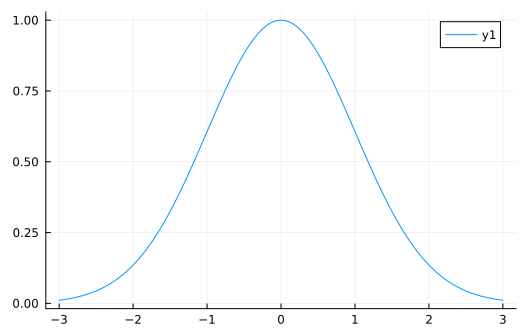
\includegraphics{./graficos_files/figure-pdf/cell-2-output-1.png}

}

\end{figure}

\hypertarget{gruxe1ficas-de-varias-funciones}{%
\subsection{Gráficas de varias
funciones}\label{gruxe1ficas-de-varias-funciones}}

\begin{itemize}
\tightlist
\item
  \texttt{plot!(f,\ xmin,\ xmax)}: Añade la gráfica de la función de una
  variable \texttt{f} para argumentos desde \texttt{xmin} a
  \texttt{xmax} al último gráfico realizado.
\end{itemize}

\begin{Shaded}
\begin{Highlighting}[]
\ImportTok{using} \BuiltInTok{Plots}

\FunctionTok{f}\NormalTok{(x) }\OperatorTok{=} \FunctionTok{sin}\NormalTok{(x)}
\FunctionTok{g}\NormalTok{(x) }\OperatorTok{=} \FunctionTok{cos}\NormalTok{(x)}
\FunctionTok{plot}\NormalTok{(f, }\OperatorTok{{-}}\FloatTok{0}\NormalTok{, }\FloatTok{2}\NormalTok{π)}
\FunctionTok{plot!}\NormalTok{(g)}
\end{Highlighting}
\end{Shaded}

\begin{figure}[H]

{\centering 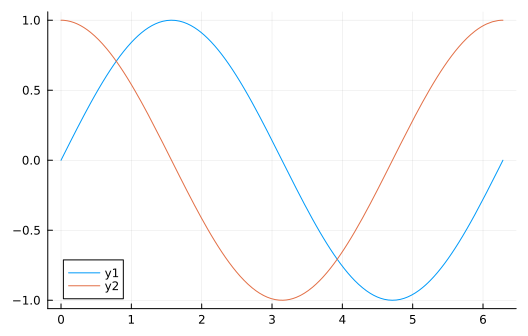
\includegraphics{./graficos_files/figure-pdf/cell-3-output-1.png}

}

\end{figure}

\hypertarget{auxf1adir-puntos-a-una-gruxe1fica}{%
\subsection{Añadir puntos a una
gráfica}\label{auxf1adir-puntos-a-una-gruxe1fica}}

\begin{itemize}
\tightlist
\item
  \texttt{scatter(x,\ y)}: Dibuja los puntos con coordenadas x en el
  vector \texttt{x} y coordenadas y en el vector \texttt{y}.
\end{itemize}

\begin{Shaded}
\begin{Highlighting}[]
\ImportTok{using} \BuiltInTok{Plots}

\FunctionTok{f}\NormalTok{(x) }\OperatorTok{=} \FunctionTok{sin}\NormalTok{(x)}
\FunctionTok{g}\NormalTok{(x) }\OperatorTok{=} \FunctionTok{cos}\NormalTok{(x)}
\FunctionTok{plot}\NormalTok{(f, }\OperatorTok{{-}}\FloatTok{0}\NormalTok{, }\FloatTok{2}\NormalTok{π)}
\FunctionTok{plot!}\NormalTok{(g)}
\NormalTok{x }\OperatorTok{=}\NormalTok{ [}\ConstantTok{π}\OperatorTok{/}\FloatTok{4}\NormalTok{, }\FloatTok{5}\NormalTok{π}\OperatorTok{/}\FloatTok{4}\NormalTok{]}
\NormalTok{y }\OperatorTok{=} \FunctionTok{sin}\NormalTok{.(x)}
\FunctionTok{scatter!}\NormalTok{(x, y)}
\end{Highlighting}
\end{Shaded}

\begin{figure}[H]

{\centering 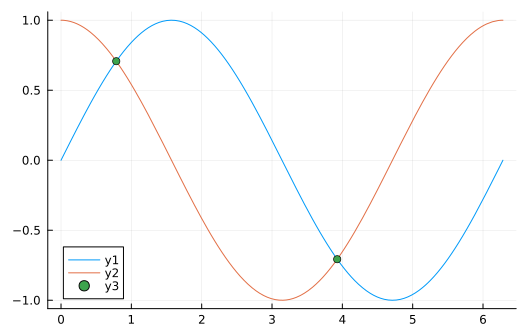
\includegraphics{./graficos_files/figure-pdf/cell-4-output-1.png}

}

\end{figure}

\hypertarget{ventana-de-graficaciuxf3n}{%
\subsection{Ventana de graficación}\label{ventana-de-graficaciuxf3n}}

Es posible restringir el área de graficación (rango de valores de los
ejes) de una función añadiendo los parámetros
\texttt{xlims\ =(xmin,\ xmax)} para establecer el rango del eje x o
\texttt{ylims\ =\ (ymin,\ ymax)} para establecer el rango del eje y.

\begin{Shaded}
\begin{Highlighting}[]
\ImportTok{using} \BuiltInTok{Plots}

\FunctionTok{f}\NormalTok{(x) }\OperatorTok{=} \FloatTok{1} \OperatorTok{/}\NormalTok{ x}
\FunctionTok{plot}\NormalTok{(f, }\OperatorTok{{-}}\FloatTok{1}\NormalTok{, }\FloatTok{1}\NormalTok{, ylims }\OperatorTok{=}\NormalTok{ (}\OperatorTok{{-}}\FloatTok{10}\NormalTok{, }\FloatTok{10}\NormalTok{))}
\end{Highlighting}
\end{Shaded}

\begin{figure}[H]

{\centering 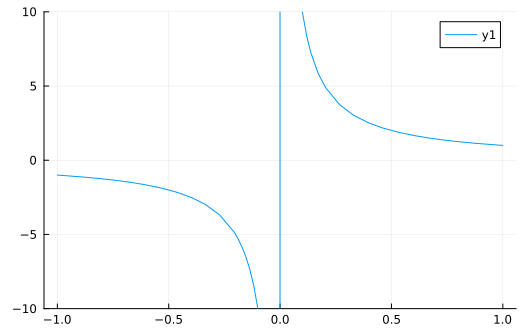
\includegraphics{./graficos_files/figure-pdf/cell-5-output-1.png}

}

\end{figure}

\hypertarget{restringir-la-gruxe1fica-al-dominio}{%
\subsection{Restringir la gráfica al
dominio}\label{restringir-la-gruxe1fica-al-dominio}}

Cuando una función no está definida para algún valor del rango de
valores del eje x dado, la gráfica muestra una línea recta desde el
punto de la gráfica anterior hasta el punto siguiente al punto donde la
función no existe.

Este comportamiento no es deseable puesto que si la función no existe en
un punto no debería existir gráfica para ese punto.

La siguiente función del paquete \texttt{MATH229} se encarga de evitar
esto.

\begin{itemize}
\tightlist
\item
  \texttt{rangeclamp(f)}: Devuelve una función idéntica a la función
  \texttt{f} excepto para los puntos donde la función no existe o es
  infinito que devuelve \texttt{NaN}.
\end{itemize}

\hypertarget{ejemplo-de-restringir-la-gruxe1fica-al-dominio}{%
\subsection{Ejemplo de restringir la gráfica al
dominio}\label{ejemplo-de-restringir-la-gruxe1fica-al-dominio}}

\begin{Shaded}
\begin{Highlighting}[]
\ImportTok{using} \BuiltInTok{Plots}
\ImportTok{using} \BuiltInTok{MTH229}

\FunctionTok{f}\NormalTok{(x) }\OperatorTok{=} \FloatTok{1} \OperatorTok{/}\NormalTok{ x}
\FunctionTok{plot}\NormalTok{(}\FunctionTok{rangeclamp}\NormalTok{(f), }\OperatorTok{{-}}\FloatTok{1}\NormalTok{, }\FloatTok{1}\NormalTok{)}
\end{Highlighting}
\end{Shaded}

\begin{figure}[H]

{\centering 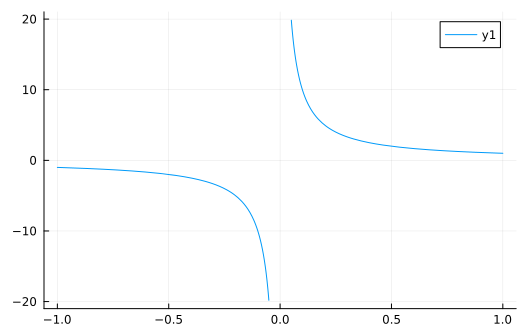
\includegraphics{./graficos_files/figure-pdf/cell-6-output-1.png}

}

\end{figure}

\hypertarget{gruxe1ficas-paramuxe9tricas}{%
\subsection{Gráficas paramétricas}\label{gruxe1ficas-paramuxe9tricas}}

La función \texttt{plot} también permite dibujar gráficas de funciones
paramétricas pasándole las funciones de las coordenadas x e y.

\begin{itemize}
\tightlist
\item
  \texttt{plot(f,\ g,\ min,\ max)}: Dibuja la gráfica de la función
  paramétrica \((f(t), g(t))\) para valores del parámetro \texttt{t}
  entre \texttt{min} y \texttt{max}.
\end{itemize}

\begin{Shaded}
\begin{Highlighting}[]
\ImportTok{using} \BuiltInTok{Plots}
\FunctionTok{f}\NormalTok{(x) }\OperatorTok{=} \FunctionTok{sin}\NormalTok{(x)}
\FunctionTok{g}\NormalTok{(x) }\OperatorTok{=} \FunctionTok{sin}\NormalTok{(}\FloatTok{2}\NormalTok{x)}
\FunctionTok{plot}\NormalTok{(f, g, }\FloatTok{0}\NormalTok{, }\FloatTok{2}\NormalTok{π)}
\end{Highlighting}
\end{Shaded}

\begin{figure}[H]

{\centering 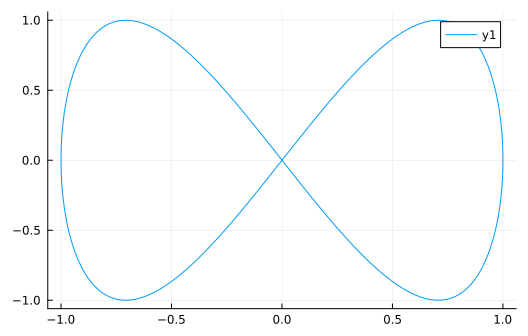
\includegraphics{./graficos_files/figure-pdf/cell-7-output-1.png}

}

\end{figure}

\hypertarget{personalizaciuxf3n-de-gruxe1ficos}{%
\subsection{Personalización de
gráficos}\label{personalizaciuxf3n-de-gruxe1ficos}}

Los siguientes parámetros pueden añadirse a la función \texttt{plot}
para modificar el aspecto de los gráficos.

\begin{itemize}
\tightlist
\item
  \texttt{title}: Añade un título principal al gráfico.
\item
  \texttt{xlab}: Añade un título al eje x.
\item
  \texttt{ylab}: Añade un título al eje y.
\item
  \texttt{color}: Establece el color de la gráfica.
\item
  \texttt{linewidth}: Establece el grosor de la línea de la gráfica.
\item
  \texttt{linestyle}: Establece el estilo de la línea de la gráfica.
\item
  \texttt{aspect\_ratio}: Establece la relación de aspecto entre la
  escala de los ejes.
\item
  \texttt{legend}: Activa o desactiva la leyenda del gráfico.
\end{itemize}

\hypertarget{ejemplo-de-personalizaciuxf3n-de-gruxe1ficos}{%
\subsection{Ejemplo de personalización de
gráficos}\label{ejemplo-de-personalizaciuxf3n-de-gruxe1ficos}}

\begin{Shaded}
\begin{Highlighting}[]
\ImportTok{using} \BuiltInTok{Plots}

\FunctionTok{f}\NormalTok{(x) }\OperatorTok{=} \FunctionTok{sin}\NormalTok{(x)}
\FunctionTok{plot}\NormalTok{(f, }\OperatorTok{{-}}\ConstantTok{π}\NormalTok{, }\ConstantTok{π}\NormalTok{, title }\OperatorTok{=} \StringTok{"Gráfica del seno"}\NormalTok{,  xlab }\OperatorTok{=} \StringTok{"x"}\NormalTok{, ylab }\OperatorTok{=} \StringTok{"f(x) = sen(x)"}\NormalTok{,}
\NormalTok{  color }\OperatorTok{=} \StringTok{"green"}\NormalTok{, linewidth }\OperatorTok{=} \FloatTok{3}\NormalTok{, linestyle }\OperatorTok{=} \OperatorTok{:}\NormalTok{dash, aspec\_ratio }\OperatorTok{=} \OperatorTok{:}\NormalTok{equal, legend }\OperatorTok{=} \ConstantTok{false}\NormalTok{)}
\end{Highlighting}
\end{Shaded}

\begin{figure}[H]

{\centering 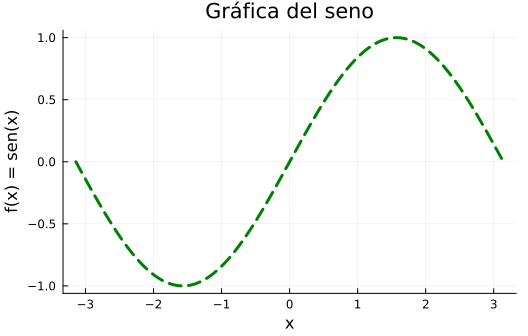
\includegraphics{./graficos_files/figure-pdf/cell-8-output-1.png}

}

\end{figure}

\hypertarget{gruxe1ficos-en-el-espacio-real}{%
\section{Gráficos en el espacio
real}\label{gruxe1ficos-en-el-espacio-real}}

Para dibujar superficies en el espacio real se utiliza la función

\texttt{surface(x,\ y,\ f)}: Dibuja la superficie de la función
\(f(x,y)\) en el rango de valores \texttt{x} del eje x e \texttt{y} del
eje y.

\begin{Shaded}
\begin{Highlighting}[]
\ImportTok{using} \BuiltInTok{Plots}
\FunctionTok{pyplot}\NormalTok{()}
\NormalTok{x }\OperatorTok{=} \FunctionTok{range}\NormalTok{(}\FloatTok{1}\NormalTok{, stop}\OperatorTok{=}\FloatTok{10}\NormalTok{, length}\OperatorTok{=}\FloatTok{100}\NormalTok{)}
\NormalTok{y }\OperatorTok{=}\NormalTok{ x}
\FunctionTok{f}\NormalTok{(x,y) }\OperatorTok{=} \FunctionTok{sin}\NormalTok{(x) }\OperatorTok{+} \FunctionTok{cos}\NormalTok{(y)}
\FunctionTok{plot}\NormalTok{(x, y, f, st}\OperatorTok{=:}\NormalTok{surface)}
\end{Highlighting}
\end{Shaded}

\begin{figure}[H]

{\centering 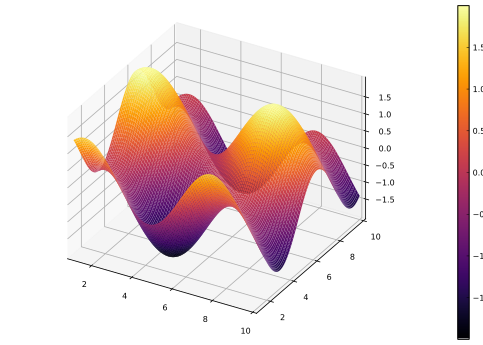
\includegraphics{./graficos_files/figure-pdf/cell-9-output-1.png}

}

\end{figure}

\hypertarget{gruxe1ficos-con-gadfly.jl}{%
\section{Gráficos con GadFly.jl}\label{gruxe1ficos-con-gadfly.jl}}

\href{http://gadflyjl.org/}{GadFly.js} es un paquete nativo que genera
gráficos interactivos 2D y 3D por medio de librerías de Javascript
basadas en la
\href{https://www.cs.uic.edu/~wilkinson/TheGrammarOfGraphics/GOG.html}{gramática
de gráficos} (usada también por el paquete ggplot2 de R).

Al estar implementado en Julia es mucho más rápido que Plots.js pero
ofrece menos posibilidades.

\includegraphics{./img/logos/gadfly.svg}

\hypertarget{gruxe1ficos-con-vegalite.jl}{%
\section{Gráficos con VegaLite.jl}\label{gruxe1ficos-con-vegalite.jl}}

\href{https://www.queryverse.org/VegaLite.jl/stable/}{VegaLite.jl} es un
paquete que genera gráficos estáticos por medio de las librerías de
Javascript de la gramática de gráficos
\href{https://vega.github.io/}{Vega}.

Dispone de muchas más opciones de personalización de gráficos que
GadFly.jl.

\includegraphics{./img/logos/vega-little.png}

\bookmarksetup{startatroot}

\hypertarget{cuxe1lculo-simbuxf3lico}{%
\chapter{Cálculo simbólico}\label{cuxe1lculo-simbuxf3lico}}

\hypertarget{symbolics.jl}{%
\section{Symbolics.jl}\label{symbolics.jl}}

\texttt{Symbolics.jl} es un paquete que implementa un avanzado Sistema
de Álgebra Computacional (CAS) basado en un lenguaje de modelado
simbólico.

Las variables y las expresiones simbólicas pueden utilizarse con la
mayoría de las funciones de Julia para cálculo numérico, por lo que se
integran a la perfección en el ecosistema de Julia.

\includegraphics{./img/logos/juliasymbolics.png}

\hypertarget{variables-y-expresiones-simbuxf3licas}{%
\subsection{Variables y expresiones
simbólicas}\label{variables-y-expresiones-simbuxf3licas}}

Para declarar variables simbólicas se utiliza la siguiente macro:

\begin{itemize}
\tightlist
\item
  \texttt{variables\ x\ y\ ...}: Declara las variables \texttt{x},
  \texttt{y}, etc. como variables simbólicas.
\end{itemize}

El tipo de las variables simbólicas es \texttt{Num}.

Cualquier expresión en la que interviene una variable simbólica se
convierte automáticamente en una expresión simbólica.

\hypertarget{ejemplo-de-variables-y-expresiones-simbuxf3licas}{%
\subsection{Ejemplo de variables y expresiones
simbólicas}\label{ejemplo-de-variables-y-expresiones-simbuxf3licas}}

\begin{Shaded}
\begin{Highlighting}[]
\ImportTok{using} \BuiltInTok{Symbolics}

\NormalTok{julia}\OperatorTok{\textgreater{}} \PreprocessorTok{@variables}\NormalTok{ x y}
\FloatTok{2}\OperatorTok{{-}}\NormalTok{element }\DataTypeTok{Vector}\NormalTok{\{Num\}}\OperatorTok{:}
\NormalTok{ x}
\NormalTok{ y}

\NormalTok{julia}\OperatorTok{\textgreater{}}\NormalTok{ z }\OperatorTok{=}\NormalTok{ x}\OperatorTok{\^{}}\FloatTok{2} \OperatorTok{{-}}\NormalTok{ y}
\NormalTok{x}\OperatorTok{\^{}}\FloatTok{2} \OperatorTok{{-}}\NormalTok{ y}

\NormalTok{julia}\OperatorTok{\textgreater{}} \FunctionTok{typeof}\NormalTok{(z)}
\NormalTok{Num}

\NormalTok{julia}\OperatorTok{\textgreater{}}\NormalTok{ A }\OperatorTok{=}\NormalTok{ [x }\OperatorTok{+}\NormalTok{ y }\FloatTok{2}\NormalTok{x; }\OperatorTok{{-}}\NormalTok{y y }\OperatorTok{{-}}\NormalTok{ x]  }\CommentTok{\# Matriz simbólica}
\FloatTok{2}\OperatorTok{×}\FloatTok{2} \DataTypeTok{Matrix}\NormalTok{\{Num\}}\OperatorTok{:}
\NormalTok{ x }\OperatorTok{+}\NormalTok{ y     }\FloatTok{2}\NormalTok{x}
    \OperatorTok{{-}}\NormalTok{y  y }\OperatorTok{{-}}\NormalTok{ x}
\end{Highlighting}
\end{Shaded}

\hypertarget{uxe1lgebra-simbuxf3lica}{%
\subsection{Álgebra simbólica}\label{uxe1lgebra-simbuxf3lica}}

Se pueden realizar operaciones algebraicas con expresiones simbólicas
utilizando los mismos operadores del Álgebra numérica.

\begin{Shaded}
\begin{Highlighting}[]
\ImportTok{using} \BuiltInTok{Symbolics}

\NormalTok{julia}\OperatorTok{\textgreater{}} \PreprocessorTok{@variables}\NormalTok{ x y;}

\NormalTok{julia}\OperatorTok{\textgreater{}}\NormalTok{ (x }\OperatorTok{+} \FloatTok{1}\NormalTok{) }\OperatorTok{+}\NormalTok{ (x }\OperatorTok{+} \FloatTok{2}\NormalTok{)}
\FloatTok{3} \OperatorTok{+} \FloatTok{2}\NormalTok{x}

\NormalTok{julia}\OperatorTok{\textgreater{}}\NormalTok{ A }\OperatorTok{=}\NormalTok{ [x }\OperatorTok{+}\NormalTok{ y }\FloatTok{2}\NormalTok{x; }\OperatorTok{{-}}\NormalTok{y y }\OperatorTok{{-}}\NormalTok{ x]  }\CommentTok{\# Matriz simbólica}
\FloatTok{2}\OperatorTok{×}\FloatTok{2} \DataTypeTok{Matrix}\NormalTok{\{Num\}}\OperatorTok{:}
\NormalTok{ x }\OperatorTok{+}\NormalTok{ y     }\FloatTok{2}\NormalTok{x}
    \OperatorTok{{-}}\NormalTok{y  y }\OperatorTok{{-}}\NormalTok{ x}

\NormalTok{julia}\OperatorTok{\textgreater{}}\NormalTok{ B }\OperatorTok{=}\NormalTok{ [x, y]  }\CommentTok{\# Vector simbólico}
\FloatTok{2}\OperatorTok{{-}}\NormalTok{element }\DataTypeTok{Vector}\NormalTok{\{Num\}}\OperatorTok{:}
\NormalTok{ x}
\NormalTok{ y}

\NormalTok{julia}\OperatorTok{\textgreater{}}\NormalTok{ A }\OperatorTok{*}\NormalTok{ B  }\CommentTok{\# Producto matricial}
\FloatTok{2}\OperatorTok{{-}}\NormalTok{element }\DataTypeTok{Vector}\NormalTok{\{Num\}}\OperatorTok{:}
 \FunctionTok{x*}\NormalTok{(x }\OperatorTok{+}\NormalTok{ y) }\OperatorTok{+} \FloatTok{2}\NormalTok{x}\OperatorTok{*}\NormalTok{y}
  \FunctionTok{y*}\NormalTok{(y }\OperatorTok{{-}}\NormalTok{ x) }\OperatorTok{{-}}\NormalTok{ x}\OperatorTok{*}\NormalTok{y}
\end{Highlighting}
\end{Shaded}

\hypertarget{simplificaciuxf3n-de-expresiones}{%
\subsection{Simplificación de
expresiones}\label{simplificaciuxf3n-de-expresiones}}

Para simplificar expresiones simbólicas se utiliza la siguiente función:

\begin{itemize}
\tightlist
\item
  \texttt{simplify(e)}: Devuelve la expresión simbólica que resulta de
  simplificar la expresión simbólica \texttt{e}.
\end{itemize}

La simplificación utiliza el paquete \texttt{SymbolicUtils.jl} que
implementa un potente sistema de reescritura de términos.

\begin{Shaded}
\begin{Highlighting}[]
\ImportTok{using} \BuiltInTok{Symbolics}

\PreprocessorTok{@variables}\NormalTok{ x y;}

\NormalTok{julia}\OperatorTok{\textgreater{}} \FunctionTok{simplify}\NormalTok{(}\FloatTok{2}\NormalTok{(x}\OperatorTok{+}\NormalTok{y))}
\FloatTok{2}\NormalTok{x }\OperatorTok{+} \FloatTok{2}\NormalTok{y}

\NormalTok{julia}\OperatorTok{\textgreater{}} \FunctionTok{simplify}\NormalTok{(}\FloatTok{2}\NormalTok{(x}\OperatorTok{+}\NormalTok{y))}
\FloatTok{2}\NormalTok{x }\OperatorTok{+} \FloatTok{2}\NormalTok{y}

\NormalTok{julia}\OperatorTok{\textgreater{}} \FunctionTok{simplify}\NormalTok{(}\FunctionTok{sin}\NormalTok{(x)}\OperatorTok{\^{}}\FloatTok{2} \OperatorTok{+} \FunctionTok{cos}\NormalTok{(x)}\OperatorTok{\^{}}\FloatTok{2}\NormalTok{)}
\FloatTok{1}
\end{Highlighting}
\end{Shaded}

\hypertarget{sustituciuxf3n-de-variables-en-expresiones}{%
\subsection{Sustitución de variables en
expresiones}\label{sustituciuxf3n-de-variables-en-expresiones}}

Para sustituir una variable simbólica en una expresión se utiliza la
siguiente función:

\begin{itemize}
\tightlist
\item
  \texttt{substitute(e,\ d)}: Realiza la sustitución de las claves por
  los valores del diccionario \texttt{d} en la expresión simbólica
  \texttt{e}.
\end{itemize}

\begin{Shaded}
\begin{Highlighting}[]
\ImportTok{using} \BuiltInTok{Symbolics}

\PreprocessorTok{@variables}\NormalTok{ x y;}

\NormalTok{julia}\OperatorTok{\textgreater{}} \FunctionTok{substitute}\NormalTok{(}\FunctionTok{cos}\NormalTok{(}\FloatTok{2}\NormalTok{x), }\FunctionTok{Dict}\NormalTok{([x }\OperatorTok{=\textgreater{}} \ConstantTok{π}\NormalTok{])) }
\FloatTok{1.0}

\NormalTok{julia}\OperatorTok{\textgreater{}} \FunctionTok{substitute}\NormalTok{(x }\OperatorTok{*}\NormalTok{ y }\OperatorTok{+} \FloatTok{2}\NormalTok{x }\OperatorTok{{-}}\NormalTok{y }\OperatorTok{+} \FloatTok{2}\NormalTok{, }\FunctionTok{Dict}\NormalTok{([x }\OperatorTok{=\textgreater{}} \FloatTok{1}\NormalTok{, y }\OperatorTok{=\textgreater{}} \FloatTok{2}\NormalTok{]))}
\FloatTok{4}
\end{Highlighting}
\end{Shaded}

\hypertarget{resoluciuxf3n-de-ecuaciones}{%
\subsection{Resolución de
ecuaciones}\label{resoluciuxf3n-de-ecuaciones}}

Para definir una ecuación se utiliza el símbolo
\texttt{\textasciitilde{}} en lugar de la igualdad.

Para resolver una ecuación se utiliza la siguiente función:

\begin{itemize}
\tightlist
\item
  \texttt{Symbolics.solve\_for(eq,\ var)}: Devuelve un vector con los
  valores de las variables del vector \texttt{var} que cumplen la
  ecuación o sistema de ecuaciones \texttt{eq}, siempre que la ecuación
  tenga solución.
\end{itemize}

\begin{tcolorbox}[enhanced jigsaw, colbacktitle=quarto-callout-warning-color!10!white, coltitle=black, opacityback=0, opacitybacktitle=0.6, bottomtitle=1mm, leftrule=.75mm, toprule=.15mm, bottomrule=.15mm, toptitle=1mm, breakable, colframe=quarto-callout-warning-color-frame, colback=white, rightrule=.15mm, titlerule=0mm, title=\textcolor{quarto-callout-warning-color}{\faExclamationTriangle}\hspace{0.5em}{Warning}, arc=.35mm, left=2mm]
Actualmente solo funciona para ecuaciones lineales.
\end{tcolorbox}

\begin{Shaded}
\begin{Highlighting}[]
\ImportTok{using} \BuiltInTok{Symbolics}

\PreprocessorTok{@variables}\NormalTok{ x y;}

\NormalTok{julia}\OperatorTok{\textgreater{}}\NormalTok{ Symbolics.}\FunctionTok{solve\_for}\NormalTok{(x }\OperatorTok{+}\NormalTok{ y }\OperatorTok{\textasciitilde{}} \FloatTok{0}\NormalTok{, x)}
\OperatorTok{{-}}\NormalTok{y}

\NormalTok{julia}\OperatorTok{\textgreater{}}\NormalTok{ Symbolics.}\FunctionTok{solve\_for}\NormalTok{([x }\OperatorTok{+}\NormalTok{ y }\OperatorTok{\textasciitilde{}} \FloatTok{4}\NormalTok{, x }\OperatorTok{{-}}\NormalTok{ y }\OperatorTok{\textasciitilde{}} \FloatTok{2}\NormalTok{], [x, y])}
\FloatTok{2}\OperatorTok{{-}}\NormalTok{element }\DataTypeTok{Vector}\NormalTok{\{}\DataTypeTok{Float64}\NormalTok{\}}\OperatorTok{:}
 \FloatTok{3.0}
 \FloatTok{1.0}
\end{Highlighting}
\end{Shaded}

\hypertarget{cuxe1lculo-de-derivadas}{%
\subsection{Cálculo de derivadas}\label{cuxe1lculo-de-derivadas}}

Para calcular la derivada de una función se utiliza la siguiente
función:

\begin{itemize}
\tightlist
\item
  \texttt{Symbolics.derivative(f,\ x)}: Devuelve la expresión simbólica
  de la derivada de la función \texttt{f} con respecto a la variable
  simbólica \texttt{x}.
\end{itemize}

\begin{Shaded}
\begin{Highlighting}[]
\ImportTok{using} \BuiltInTok{Symbolics}

\NormalTok{julia}\OperatorTok{\textgreater{}} \PreprocessorTok{@variables}\NormalTok{ x y;}

\NormalTok{julia}\OperatorTok{\textgreater{}}\NormalTok{ Symbolics.}\FunctionTok{derivative}\NormalTok{(}\FunctionTok{exp}\NormalTok{(x}\OperatorTok{*}\NormalTok{y), x)}
\FunctionTok{y*exp}\NormalTok{(x}\OperatorTok{*}\NormalTok{y)}

\NormalTok{julia}\OperatorTok{\textgreater{}}\NormalTok{ Symbolics.}\FunctionTok{derivative}\NormalTok{(Symbolics.}\FunctionTok{derivative}\NormalTok{(}\FunctionTok{exp}\NormalTok{(x}\OperatorTok{*}\NormalTok{y), x), y)}
\FunctionTok{x*y*exp}\NormalTok{(x}\OperatorTok{*}\NormalTok{y) }\OperatorTok{+} \FunctionTok{exp}\NormalTok{(x}\OperatorTok{*}\NormalTok{y)}
\end{Highlighting}
\end{Shaded}

\hypertarget{cuxe1lculo-de-derivadas-con-operadores-diferenciales}{%
\subsection{Cálculo de derivadas con operadores
diferenciales}\label{cuxe1lculo-de-derivadas-con-operadores-diferenciales}}

Para construir un operador diferencial (\(\frac{d}{dx}\)) se utiliza la
siguiente función:

\begin{itemize}
\tightlist
\item
  \texttt{Differential(x)}: Crea el operador diferencial con respecto a
  la variable simbólica \texttt{x}.
\end{itemize}

Para obtener la función derivada, una vez aplicado el operador
diferencial a una función, es necesario aplicar la siguiente función:

\begin{itemize}
\tightlist
\item
  \texttt{expand\_derivatives(D(f))}: Devuelve la expresión simbólica
  que corresponde a la derivada de la función \texttt{f} con respecto a
  la variable del operador diferencial \texttt{D}.
\end{itemize}

\hypertarget{ejemplo-de-cuxe1lculo-de-derivadas-con-operadores-diferenciales}{%
\subsection{Ejemplo de cálculo de derivadas con operadores
diferenciales}\label{ejemplo-de-cuxe1lculo-de-derivadas-con-operadores-diferenciales}}

\begin{Shaded}
\begin{Highlighting}[]
\ImportTok{using} \BuiltInTok{Symbolics}

\PreprocessorTok{@variables}\NormalTok{ x y;}

\NormalTok{julia}\OperatorTok{\textgreater{}}\NormalTok{ Dx }\OperatorTok{=} \FunctionTok{Differential}\NormalTok{(x)}
\NormalTok{(}\OperatorTok{::}\DataTypeTok{Differential}\NormalTok{) (generic }\KeywordTok{function}\NormalTok{ with }\FloatTok{2}\NormalTok{ methods)}

\NormalTok{julia}\OperatorTok{\textgreater{}} \FunctionTok{f}\NormalTok{(x) }\OperatorTok{=} \FunctionTok{sin}\NormalTok{(x}\OperatorTok{\^{}}\FloatTok{2}\NormalTok{)}
\NormalTok{f (generic }\KeywordTok{function}\NormalTok{ with }\FloatTok{1}\NormalTok{ method)}

\NormalTok{julia}\OperatorTok{\textgreater{}} \FunctionTok{f1}\NormalTok{(x) }\OperatorTok{=} \FunctionTok{Dx}\NormalTok{(}\FunctionTok{f}\NormalTok{(x))}
\NormalTok{f1 (generic }\KeywordTok{function}\NormalTok{ with }\FloatTok{1}\NormalTok{ method)}

\NormalTok{julia}\OperatorTok{\textgreater{}} \FunctionTok{expand\_derivatives}\NormalTok{(}\FunctionTok{f1}\NormalTok{(x))}
\FloatTok{2}\FunctionTok{x*cos}\NormalTok{(x}\OperatorTok{\^{}}\FloatTok{2}\NormalTok{)}

\NormalTok{julia}\OperatorTok{\textgreater{}}\NormalTok{ Dy }\OperatorTok{=} \FunctionTok{Differential}\NormalTok{(y)}
\NormalTok{(}\OperatorTok{::}\DataTypeTok{Differential}\NormalTok{) (generic }\KeywordTok{function}\NormalTok{ with }\FloatTok{2}\NormalTok{ methods)}

\NormalTok{julia}\OperatorTok{\textgreater{}} \FunctionTok{expand\_derivatives}\NormalTok{(}\FunctionTok{Dx}\NormalTok{(}\FunctionTok{Dy}\NormalTok{(}\FunctionTok{cos}\NormalTok{(x}\OperatorTok{*}\NormalTok{y))))}
\FunctionTok{{-}sin}\NormalTok{(x}\OperatorTok{*}\NormalTok{y) }\OperatorTok{{-}} \FunctionTok{x*y*cos}\NormalTok{(x}\OperatorTok{*}\NormalTok{y)}
\end{Highlighting}
\end{Shaded}

\hypertarget{gradiente-y-matriz-hessiana-de-una-funciuxf3n-de-varias-variables}{%
\subsection{Gradiente y matriz Hessiana de una función de varias
variables}\label{gradiente-y-matriz-hessiana-de-una-funciuxf3n-de-varias-variables}}

Para calcular el vector gradiente de una función de varias variables se
utiliza la siguiente función:

\begin{itemize}
\tightlist
\item
  \texttt{Symbolics.gradient(f,\ vars)}: Devuelve el vector gradiente de
  la función \texttt{f} con respecto a las variables del vector
  \texttt{vars}.
\end{itemize}

Y para calcular la matriz Hessiana se utiliza la siguiente función:

\begin{itemize}
\tightlist
\item
  \texttt{Symbolics.hessian(f,\ vars)}: Devuelve la matriz Hessiana de
  la función \texttt{f} con respecto a las variables del vector
  \texttt{vars}.
\end{itemize}

\hypertarget{ejemplo-de-gradiente-y-matriz-hessiana-de-una-funciuxf3n-de-varias-variables}{%
\subsection{Ejemplo de gradiente y matriz Hessiana de una función de
varias
variables}\label{ejemplo-de-gradiente-y-matriz-hessiana-de-una-funciuxf3n-de-varias-variables}}

\begin{Shaded}
\begin{Highlighting}[]
\ImportTok{using} \BuiltInTok{Symbolics}

\PreprocessorTok{@variables}\NormalTok{ x y;}

\NormalTok{julia}\OperatorTok{\textgreater{}}\NormalTok{ Symbolics.}\FunctionTok{gradient}\NormalTok{(}\FunctionTok{exp}\NormalTok{(x}\OperatorTok{*}\NormalTok{y), [x, y])}
\FloatTok{2}\OperatorTok{{-}}\NormalTok{element }\DataTypeTok{Vector}\NormalTok{\{Num\}}\OperatorTok{:}
 \FunctionTok{y*exp}\NormalTok{(x}\OperatorTok{*}\NormalTok{y)}
 \FunctionTok{x*exp}\NormalTok{(x}\OperatorTok{*}\NormalTok{y)}

\NormalTok{julia}\OperatorTok{\textgreater{}}\NormalTok{ Symbolics.}\FunctionTok{hessian}\NormalTok{(}\FunctionTok{exp}\NormalTok{(x}\OperatorTok{*}\NormalTok{y), [x, y])}
\FloatTok{2}\OperatorTok{×}\FloatTok{2} \DataTypeTok{Matrix}\NormalTok{\{Num\}}\OperatorTok{:}
\NormalTok{ (y}\OperatorTok{\^{}}\FloatTok{2}\NormalTok{)}\FunctionTok{*exp}\NormalTok{(x}\OperatorTok{*}\NormalTok{y)               }\FunctionTok{x*y*exp}\NormalTok{(x}\OperatorTok{*}\NormalTok{y) }\OperatorTok{+} \FunctionTok{exp}\NormalTok{(x}\OperatorTok{*}\NormalTok{y)}
   \FunctionTok{x*y*exp}\NormalTok{(x}\OperatorTok{*}\NormalTok{y) }\OperatorTok{+} \FunctionTok{exp}\NormalTok{(x}\OperatorTok{*}\NormalTok{y)  (x}\OperatorTok{\^{}}\FloatTok{2}\NormalTok{)}\FunctionTok{*exp}\NormalTok{(x}\OperatorTok{*}\NormalTok{y)}
\end{Highlighting}
\end{Shaded}

\bookmarksetup{startatroot}

\hypertarget{anuxe1lisis-de-datos}{%
\chapter{Análisis de datos}\label{anuxe1lisis-de-datos}}

\hypertarget{el-paquete-dataframes.jl}{%
\section{El paquete DataFrames.jl}\label{el-paquete-dataframes.jl}}

El principal paquete para análisis de datos es
\href{https://dataframes.juliadata.org/stable/}{\texttt{DataFrames.jl}}
que proporciona herramientas para trabajar con conjuntos de datos en
formato de tabla de forma similar a pandas en Python o data.frames y
dplyr en R.

En conjunción con este paquete es frecuente utilizar también alguno de
los siguientes paquetes:

\begin{itemize}
\tightlist
\item
  \href{https://github.com/nalimilan/FreqTables.jl}{FreqTables.jl}.
  Funciones para la construcción de tablas de frecuencias.
\item
  \href{https://docs.julialang.org/en/v1/stdlib/Statistics/}{Statistics.jl}.
  Funciones para los principales estadísticos descriptivos.
\item
  \href{https://juliastats.org/HypothesisTests.jl/stable/}{HypothesisTests.jl}
  Funciones para los contrastes de hipótesis paramétricos y no
  paramétricos más comunes.
\item
  \href{https://juliastats.org/GLM.jl/stable/}{GLM.jl}. Funciones para
  modelos lineales generales.
\item
  \href{https://multivariatestatsjl.readthedocs.io/en/stable/index.html}{MultivariateStats.jl}.
  Funciones para análisis multivariante.
\item
  \href{https://github.com/alan-turing-institute/MLJ.jl}{MLJ.jl}.
  Funciones para los principales algoritmos de aprendizaje automático.
\end{itemize}

\hypertarget{creaciuxf3n-de-dataframes}{%
\subsection{Creación de DataFrames}\label{creaciuxf3n-de-dataframes}}

Para crear un DataFrame su utiliza la siguiente función:

\begin{itemize}
\tightlist
\item
  \texttt{DataFrame(x1=v1,\ x2=v2,\ ...)}: Devuelve el DataFrame que
  formado por las columnas de los vectores \texttt{v1}, \texttt{v2},
  etc, con los nombres \texttt{x1}, \texttt{x2}, etc, respectivamente.
\end{itemize}

\begin{Shaded}
\begin{Highlighting}[]
\ImportTok{using} \BuiltInTok{DataFrames}

\NormalTok{julia}\OperatorTok{\textgreater{}}\NormalTok{ df }\OperatorTok{=} \FunctionTok{DataFrame}\NormalTok{(Nombre }\OperatorTok{=}\NormalTok{ [}\StringTok{"María"}\NormalTok{, }\StringTok{"Luis"}\NormalTok{, }\StringTok{"Carmen"}\NormalTok{], Edad }\OperatorTok{=}\NormalTok{ [}\FloatTok{22}\NormalTok{, }\FloatTok{18}\NormalTok{, }\FloatTok{20}\NormalTok{])}
\FloatTok{3}\OperatorTok{×}\FloatTok{2}\NormalTok{ DataFrame}
\NormalTok{ Row │ Nombre  Edad  }
\NormalTok{     │ }\DataTypeTok{String}  \DataTypeTok{Int64} 
\NormalTok{─────┼───────────────}
   \FloatTok{1}\NormalTok{ │ María      }\FloatTok{22}
   \FloatTok{2}\NormalTok{ │ Luis       }\FloatTok{18}
   \FloatTok{3}\NormalTok{ │ Carmen     }\FloatTok{20}
\end{Highlighting}
\end{Shaded}

\hypertarget{creaciuxf3n-de-dataframes-desde-una-url}{%
\subsection{Creación de DataFrames desde una
url}\label{creaciuxf3n-de-dataframes-desde-una-url}}

Para crear una DataFrame a partir de un fichero csv en la nube, se
utiliza la siguiente función del paquete \texttt{CSV.jl}:

\begin{itemize}
\tightlist
\item
  \texttt{CSV.read(download(url),\ DataFrame)}: Devuelve el DataFrame
  que resulta de importar el fichero csv con la url \texttt{url}.
\end{itemize}

\begin{Shaded}
\begin{Highlighting}[]
\ImportTok{using} \BuiltInTok{DataFrames}\NormalTok{, }\BuiltInTok{CSV}

\NormalTok{julia}\OperatorTok{\textgreater{}}\NormalTok{ df }\OperatorTok{=}\NormalTok{ CSV.}\FunctionTok{read}\NormalTok{(}\FunctionTok{download}\NormalTok{(}\StringTok{"https://raw.githubusercontent.com/asalber/manual{-}python/master/datos/colesteroles.csv"}\NormalTok{), DataFrame)}
\FloatTok{14}\OperatorTok{×}\FloatTok{6}\NormalTok{ DataFrame}
\NormalTok{ Row │ nombre                           edad   sexo     peso     altura   colesterol }
\NormalTok{     │ }\DataTypeTok{String}                           \DataTypeTok{Int64}\NormalTok{  String1  }\DataTypeTok{Int64}\NormalTok{?   String7  }\DataTypeTok{Int64}\NormalTok{?     }
\NormalTok{─────┼───────────────────────────────────────────────────────────────────────────────}
   \FloatTok{1}\NormalTok{ │ José Luis Martínez Izquierdo        }\FloatTok{18}\NormalTok{  H             }\FloatTok{85}  \FloatTok{1}\NormalTok{,}\FloatTok{79}            \FloatTok{182}
   \FloatTok{2}\NormalTok{ │ Rosa Díaz Díaz                      }\FloatTok{32}\NormalTok{  M             }\FloatTok{65}  \FloatTok{1}\NormalTok{,}\FloatTok{73}            \FloatTok{232}
   \FloatTok{3}\NormalTok{ │ Javier García Sánchez               }\FloatTok{24}\NormalTok{  H        }\ConstantTok{missing}  \FloatTok{1}\NormalTok{,}\FloatTok{81}            \FloatTok{191}
   \FloatTok{4}\NormalTok{ │ Carmen López Pinzón                 }\FloatTok{35}\NormalTok{  M             }\FloatTok{65}  \FloatTok{1}\NormalTok{,}\FloatTok{70}            \FloatTok{200}
   \FloatTok{5}\NormalTok{ │ Marisa López Collado                }\FloatTok{46}\NormalTok{  M             }\FloatTok{51}  \FloatTok{1}\NormalTok{,}\FloatTok{58}            \FloatTok{148}
   \FloatTok{6}\NormalTok{ │ Antonio Ruiz Cruz                   }\FloatTok{68}\NormalTok{  H             }\FloatTok{66}  \FloatTok{1}\NormalTok{,}\FloatTok{74}            \FloatTok{249}
   \FloatTok{7}\NormalTok{ │ Antonio Fernández Ocaña             }\FloatTok{51}\NormalTok{  H             }\FloatTok{62}  \FloatTok{1}\NormalTok{,}\FloatTok{72}            \FloatTok{276}
   \FloatTok{8}\NormalTok{ │ Pilar Martín González               }\FloatTok{22}\NormalTok{  M             }\FloatTok{60}  \FloatTok{1}\NormalTok{,}\FloatTok{66}        \ConstantTok{missing} 
   \FloatTok{9}\NormalTok{ │ Pedro Gálvez Tenorio                }\FloatTok{35}\NormalTok{  H             }\FloatTok{90}  \FloatTok{1}\NormalTok{,}\FloatTok{94}            \FloatTok{241}
  \FloatTok{10}\NormalTok{ │ Santiago Reillo Manzano             }\FloatTok{46}\NormalTok{  H             }\FloatTok{75}  \FloatTok{1}\NormalTok{,}\FloatTok{85}            \FloatTok{280}
  \FloatTok{11}\NormalTok{ │ Macarena Álvarez Luna               }\FloatTok{53}\NormalTok{  M             }\FloatTok{55}  \FloatTok{1}\NormalTok{,}\FloatTok{62}            \FloatTok{262}
  \FloatTok{12}\NormalTok{ │ José María de la Guía Sanz          }\FloatTok{58}\NormalTok{  H             }\FloatTok{78}  \FloatTok{1}\NormalTok{,}\FloatTok{87}            \FloatTok{198}
  \FloatTok{13}\NormalTok{ │ Miguel Angel Cuadrado Gutiérrez     }\FloatTok{27}\NormalTok{  H            }\FloatTok{109}  \FloatTok{1}\NormalTok{,}\FloatTok{98}            \FloatTok{210}
  \FloatTok{14}\NormalTok{ │ Carolina Rubio Moreno               }\FloatTok{20}\NormalTok{  M             }\FloatTok{61}  \FloatTok{1}\NormalTok{,}\FloatTok{77}            \FloatTok{194}
\end{Highlighting}
\end{Shaded}

\bookmarksetup{startatroot}

\hypertarget{otras-aplicaciones}{%
\chapter{Otras aplicaciones}\label{otras-aplicaciones}}

\hypertarget{teoruxeda-de-grafos}{%
\section{Teoría de grafos}\label{teoruxeda-de-grafos}}

\begin{itemize}
\tightlist
\item
  \href{https://juliagraphs.org/}{JuliaGraphs}. Graphs analysis in
  Julia.
\end{itemize}

\hypertarget{cuxe1lculo-simbuxf3lico-1}{%
\section{Cálculo simbólico}\label{cuxe1lculo-simbuxf3lico-1}}

\begin{itemize}
\tightlist
\item
  \href{https://docs.juliahub.com/SymPy/KzewI/1.0.31/}{SymPy}. Sistema
  de Álgebra Computacional (CAS) basdado en la librería \texttt{SymPy}
  de Python.
\item
  \href{https://juliasymbolics.org/}{Symbolics} Sistema de Álgebra
  Computacional (CAS) basado en Julia.
\end{itemize}

\hypertarget{aprendizaje-automuxe1tico}{%
\section{Aprendizaje automático}\label{aprendizaje-automuxe1tico}}

\begin{itemize}
\tightlist
\item
  \href{https://github.com/alan-turing-institute/MLJ.jl}{MLJ.jl}.
  Funciones para los principales algoritmos de aprendizaje automático.
\end{itemize}

\bookmarksetup{startatroot}

\hypertarget{referencias}{%
\chapter*{Referencias}\label{referencias}}
\addcontentsline{toc}{chapter}{Referencias}

\hypertarget{refs}{}
\begin{CSLReferences}{0}{0}
\end{CSLReferences}



\end{document}
